\chapter{نتایج و تفسیر آنها}
\clearpage
\section{مقدمه}
کشف گرافن با پراکندگی خطی آن باعث شد که الکترون‌ها مانند فرمیون های بدون جرم دیراک حرکت کنند [1،2]. وجود نقاط دیراک در گرافن باعث ایجاد خواص الکترونیکی، مکانیکی و نوری متفاوتی نسبت به سایر آلوتروپ های کربن می شود [3]. شناسایی این رفتارهای جدید رویای وسایل الکترونیکی را بسیار دست یافتنی تر به نظر می رساند. از سوی دیگر، فقدان شکاف باند و تحرک بالای حامل ها، کاربرد گرافن را در دستگاه های نیمه هادی محدود می کند. بنابراین، مواد دو بعدی دیگر مانند سیلیس [4]، ژرمانن [5]، استانن [6]، فسفر سیاه [7] و آنتیمونن [8]، دی سولفید مولیبدن [9]، دیکالکوژنیدهای فلزی میانی (\ce{TMDC}) [10] و نیترید بور شش ضلعی (\ce{h-BN}) [11] به آسانی با روش های سنتز قوی در دسترس هستند و با موفقیت در کاربردهای الکترونیکی استفاده شده اند [12-14]. اخیراً، ماده دو بعدی دیگری به نام بوروفن بر روی بستر نقره [15،16] شرایط خلاء بسیار بالا بر اساس محاسبات نظری [17-19] سنتز شده است که به دلیل خواص خارقالعادهاش جلب توجه میکند. خواص مکانیکی جذاب آن را به رقیبی برای گرافن تبدیل کرده است [15]. همچنین دارای خواص فلز ناهمسانگرد است که منجر به خواص فیزیکی وابسته به جهت مناسب برای استفاده در دستگاه های انعطاف پذیر می شود.

با گذشت زمان، قانون مور برای موثر ماندن با چالش های جدی تری مواجه خواهد شد. با توجه به اینکه الکترونیک سنتی تنها بر اساس حمل و نقل و ذخیره بار الکتریکی استوار است، ادامه فرآیند کوچک سازی محدودیت های بیشتر و چالش های عمیق تری را به همراه خواهد داشت. بنابراین، دستگاه های مبتنی بر اصول جدید تبدیل به یک کانون در دوران پس از مور 1،2 شده اند. Spintronics یکی از فناوری هایی است که ممکن است قانون مور را به چالش بکشد. هدف اسپینترونیک درک برهمکنش اسپین ذرات با محیط جامد اطراف آنها، به ویژه تأثیر اسپین الکترون بر رسانایی (یا جریان) است. مشکل اصلی در اسپینترونیک ساخت دستگاه های مبتنی بر اسپینترونیک است. از زمان کشف GMR در سال 1988 3،4، اسپینترونیک از جمله STT 5،6، اسپینترونیک نیمه هادی، اسپینترونیک تک الکترونی و غیره به عنوان یک زمینه تحقیقاتی جدید فعال بوده است. یکی از شگفت انگیزترین کاربردهای اسپینترونیک اثر شیر چرخشی 5 است که با زاویه نسبی ماگا قابل دستکاری شبکه سازی لایه های مغناطیسی در لیدها. شیر چرخشی اولین بار در سال 1991 توسعه یافت، که بعداً صنعت حسگرهای مغناطیسی، هدهای دیسک سخت و حافظههای دسترسی تصادفی مغناطیسی (MRAM) 8-11 را متحول کرد. دستگاه شیر چرخشی از دو یا چند اتصال مغناطیسی تشکیل شده است. در یک دستگاه شیر چرخشی با دو اتصال مغناطیسی، بسته به اینکه اتصالات مغناطیسی در جهت جریان درون صفحه (CIP) یا عمود بر صفحه (CPP) باشد، دو ساختار هندسی متفاوت تشکیل می شود. مقاومت مغناطیسی به پدیده ای اطلاق می شود که مقاومت یک فلز یا نیمه هادی با یک میدان مغناطیسی خارجی تغییر می کند.

همچنین نشان داده شده است که نانوروبانهای دارای لبههای صندلی بدون بار لبهای هستند، زیرا اتمهای لبه آنها به یک زیرشبکه ختم میشوند. LDOS در نزدیکی انرژی فرمی، چگالی الکترونی فضایی حالتها در کل محل نانوروبان بوروفن صندلی با یک مکان خالی در لبه بالایی خالی، یک جای خالی، و دو جای خالی در وسط نانو نوار رسم شده است. نوع بنابراین، اگرچه آنها به طور کلی نیمه هادی هستند، اما حالت های صفر را می توان در عرض های به درستی انتخاب شده ایجاد کرد [58]. این باعث می شود که نانوروبان های لبه صندلی بین رفتارهای نیمه هادی و هادی در نوسان باشند. بنابراین، رفتار مشابه مشاهده شده در BNR ها را می توان به عنوان تاییدی بر وجود شبکه لانه زنبوری پنهان در نظر گرفت.

\subsection{شبکه شش گوشی پنهان}
بوروفن-$\beta_{12}$ یک ورقه گرافن مانند دوبعدی پایدار است که توسط محاسبات و آزمایشات اصول اولیه تأیید شده است [26]. ساختار $\beta_{12}$ یک شبکه مستطیل شکل با پایه ای است که دارای پنج اتم است که به صورت a، b، c، d و e در شکل \lr{1.b} شکل 2 نشان داده شده است. با تقارن P2MM ثابت های شبکه مستطیلی 2.92\AA و 5.06\AA هستند [53]، بنابراین فاصله اتمی بور-بور\ce{B-B} استl=1.69\AA. طبق محاسبات اصول اولیه\LTRfootnote{First Principle Calculations}، ثابت شبکه BNRهای بدون اتم مرکزی (بوروفن با ساختار لانه زنبوری) 0.4\% کمتر از بوروفن $\beta_{12}$ است، و چگالی بار در اطراف اتم مرکزی، در مقایسه با سطح هم سطح لانه زنبوری چگالی بار، رقیق شده است. از سوی دیگر، شش پیوند درون صفحه در $\beta_{12}$ ($\sigma$ -پیوندها) دارای تقارن انتقالی هستند. بنابراین ما شبکه ای از لانه زنبوری داریم که در $\beta_{12}$ پنهان شده است، که در آن اتم مرکزی به عنوان یک الکترون دهنده عمل می کند تا پیوندهای $\sigma$ داخل ساختار لانه زنبوری را پر کند [54]. 

اگرچه ساختار $\beta_{12}$، بر خلاف گرافن و سیلیسین، به جای ساختار شبکه شش ضلعی، دارای ساختار شبکه ای مستطیلی است، محاسبات اصل اول نشان داد که چگالی الکترونی موضعی حالات (LDOS) در $\beta_{12}$ در مرکز سلول واحد آن است. بسیار کمتر از همسایگان خود [25]، و بنابراین می توان انتظار داشت که بوروفن نیز میزبان مخروط های دیراک باشد. فرمیون های دیراک توسط آزمایش های طیف سنجی انتشار نوری با وضوح زاویه ای (ARPES) و محاسبات اصل اول مشاهده می شوند [26]. ساختار نوار به خوبی توسط یک مدل اتصال محکم بازتولید شده است، به طوری که، به دلیل ساختار مسطح کامل آن، در نظر گرفتن تنها اوربیتال های $P_z$ کافی است. اگرچه بوروفن بر روی بسترهای فلزی سنتز شده است، اما هنوز جدا نشده است، و بسیاری از درک خواص نوری الکترونیکی آن از تئوری و محاسبات ناشی می شود. به طور خاص، مطالعات تئوری تابعی چگالی (DFT) ساختار نواری آلوتروپ های مختلف بوروفن را بررسی کرده است. این مطالعات پیشبینی میکنند که ساختارهای کریستالی کم انرژی مختلف میتوانند منجر به رفتار فلزی یا نیمه فلزی شوند [25،27-30]، ممکن است حاوی مخروطهای دیراک در یا نزدیک انرژی فرمی [30-35] باشند و اغلب ناهمسانگردی رسانایی درون صفحه را نشان میدهند. به پیکربندی اتصال ناهمسانگرد [36،37]. همچنین نشان داده شده است که علاوه بر فرمیونهای دیراک، مدلهای دیراک در نقاط تماس سه باندی نیز وجود دارد و شکل صریح همیلتونهای مؤثر آنها به دست میآید [38]. مطالعات نظری زیادی روی $\beta_{12}$ انجام شده است، [39-41] از جمله پیشبینی رفتار ابررسانا در محدوده دمایی 10-20 کلوین به دلیل جرم اتمی کوچک آن، که باعث جفت شدن قوی الکترون-فونون میشود [42].
آزمایشها و محاسبات اصول اولیه نشان داده‌اند که مخروطهای دیراک از اوربیتالهای Pz مشتق شده اند. از آنجایی که تابع موج در انرژی فرمی در محل c دامنه ندارد، [26] این شش اتم اطراف فاز یکدیگر را خنثی می کنند، بنابراین شکل 3. در انرژی متناظر تا اوج LDOS در نزدیکی انرژی فرمی، چگالی الکترونی فضایی حالتها در کل محل نانوروبان بوروفن زیگزاگ با محل پراکندگی در لبه بالایی با V=0,1,2,5 در وسط نانوروبان ترسیم شده است. . 

توابع موج به دست آمده از سایت های a،b،d و e به دو زیرشبکه تقسیم می شوند. ما زیرشبکه A را به اتم های a,d و زیرشبکه B را به اتم های b,e نامیدیم. نشان داده شده است که یک مدل اتصال محکم پنج باند با انتخاب ضرایب انرژی در محل و پرش مناسب به خوبی با محاسبات اصلی اول مطابقت دارد [26،55]. در این مدل، انرژی های موجود در محل، تقارن وارونگی سازه را به دلیل تأثیرات زیرلایه Ag می شکنند و به همین دلیل به آن مدل نا متقارن وارونگی (INS) می گویند. به منظور حذف اثرات زیرلایه، یک مدل متقارن وارونگی (IS) تعریف شده و برای افزودن همگنی، یک مدل همگن معرفی شده است [38]. ما همه این ضرایب را در جدول 1 فهرست کردهایم. همیلتونین پیوندی محکم از بوروفن $\beta_{12}$ که صرفاً اوربیتالهای $P_z$ را در فضای واقعی در نظر میگیرد، میتواند به صورت زیر ارائه شود:

\begin{table}
  \centering
  \caption{پارامترهای پرش \lr{$\beta_{12}$-borophene} معرفی شده توسط \lr{Ezawa}\cite{ezawaTripletFermionsDirac2017}\label{tbl:hoppingtable}}
  \begin{tabular}{cccccccc}
  \toprule
   & H & INS & IS &
   & H & INS & IS\\
  \midrule
  $\varepsilon_a$& 0 &  0.196 &  0.196 & $t_{ab}=t_{de}$& -2 & -2.04 & -2.04 \\
  $\varepsilon_b$& 0 & -0.058 & -0.058 & $t_{ac}=t_{ce}$& -2 & -1.79 & -1.79 \\
  $\varepsilon_c$& 0 & -0.845 & -0.845 & $t_{ae}$& -2 & -2.12 & -2.12   \\
  $\varepsilon_d$& 0 &  0.196 & -0.058 & $t_{bc}=t_{cd}$& -2 & -1.84 & -1.84 \\
  $\varepsilon_e$& 0 & -0.058 &  0.196 & $t_{bd}$& -2 & -1.91 & -1.91  \\
  \bottomrule
  \end{tabular}
  \end{table}
\section{رسانش کلید ساخت وسایل الکترونیکی}
در اینجا باید اشاره کنیم که در میان تمام خاصیت هایی که مواد دوبعدی دارند رسانندگی اهمیت ویژه ای برای ساخت ریز دستگاه های اکترونیکی دارند. بنابراین رسانش را در سه حالت کلی بررسی میکنیم
۱. رسانش کوانتومی بار
۲. رسانش کوانتومی اسپین
۳. رسانش کوانتومی درهها
\section{رسانش کوانتومی بار}
طیف های انتقال نانوروبان های بوروفن بکر (BNRs) ساختار پله ای شناخته شده ای را نشان می دهد. ارتفاع پله ها مربوط به تعداد نوارهای انرژی است که از انرژی داده شده عبور می کنند. علاوه بر این، برخلاف نانوروبانهای گرافن (GNRs)، تعداد کانالهای رسانایی در انرژی فرمی ثابت نمیماند [57] و با افزایش عرض نانوروبانها افزایش مییابد که در نانوروبانهایی با لبه زیگزاگ در مقایسه با لبه صندلی صندلی یک بیشتر دیده میشود [38]. دلیل وابستگی عرض به تعداد کانال های رسانایی در انرژی فرمی را می توان به وجود اتم مرکزی در داخل سلول واحد نسبت داد. هر یک از اتم های پایه در سلول واحد نوارهای $\beta_{12}$-بوروفن می تواند روی لبه باشد و بر اساس اتم لبه، پنج نوع ابرسلول زیگزاگ در نظر گرفته می شود. وقتی اتم e روی لبه قرار می گیرد، دیگر لبه زیگزاگی نخواهد بود، بنابراین در مجموع 16 نوع ابرسلول زیگزاگ دیده می شود. میتوانیم ابرسلولها را با نام اتمهای لبههای بالا و پایین نامگذاری کنیم، مثلاً ZNBR-cd که به اتم c در لبه بالا و اتم d در لبه پایین ختم میشود. محاسبات ما نشان میدهد که اگرچه ZNBR-cd با عرض 8.8\AA دارای شکافهای باند بسیار کوچکی است، اما اغلب خواص فلزی را نشان میدهند. زیرا ابرسلول هایی که از هر دو انتها به یک سلول ختم می شوند در بسیاری از محاسبات استفاده شده اند [26،38]. در این تحقیق نیز همین ساختار مورد توجه قرار گرفته است. در مورد لبه های صندلی، هر لبه می تواند به b-d(ac-a) ختم شود که آن را به ترتیب $\alpha$ ($\gamma$) می نامیم، بنابراین چهار نوع ابرسلول صندلی داریم که یک نمونه آن\lr{ABNR-$\alpha\alpha$}است.محاسبات ما نشان می دهد که برخلاف ZBNR ها، نانوروبان های لبه صندلی دارای رفتار نیمه هادی یا فلزی وابسته به عرض روبان W هستند، به طوری که برای عرض بیشتر از مقدار بحرانی \AA $W_c = 11.08$، رسانایی را می توان یافت و برعکس یا $W\leq W_c$، سیستم مانند یک نیمه هادی رفتار می کند. وابستگی حالت های الکترونی به عرض نانوروبان ها در یک شبکه لانه زنبوری با حل معادله دیراک (شرودینگر) با شرایط مرزی مناسب، که دارای توابع موج صفر در هر دو لبه نانوروبان هستند، درک می شود. بر اساس محاسبات انجام شده مشاهده می شود که نانوروبان هایی با لبه های زیگزاگی که لبه های بالایی و پایینی آنها به زیرشبکه های مختلف ختم می شود، توابع موج لبه ایجاد می کنند. همانطور که می دانیم، بر خلاف الکترون های بلوخ، حالت های لبه به طور تصاعدی در فواصل کوتاه از لبه ها تحلیل می روند. حالت های لبه در شکاف انرژی در نیمه هادی ها و همچنین در شکاف های محلی در هادی ها قرار دارند.
%%%% این قسمت نیاز دارد که برخی از نمودارها که در مقالات نیاوردهایم بیاوریم و نتایج را حاصل محاسبات خود مطرح کنیم.

\section{رسانش کوانتومی بار نانونوارها در حضور انواع نقص}

وجود عیوب در مواد دو بعدی در حین ساخت آنها امری رایج است. به عنوان مثال، گرافن، با وجود پایداری حرارتی بالا، دارای عیوب گوناگونی در فرآیند رشد کریستال خود است [49،50]. از سوی دیگر، از آنجایی که پایداری حرارتی بوروفن کمتر از گرافن است، احتمال بروز نقص در هنگام ساخت بیشتر است [51]. بر خلاف سایر مواد دو بعدی، بوروفن اخیراً دارای فرآیندهای رشد لبه است و در حالی که شکل تعادل ترمودینامیکی آن تقریباً مستطیلی است، در مشاهدات تجربی مشاهده نشده است و در بیشتر موارد، ناهمواریهای لبه وجود دارد [52]. در نتیجه، این فرض که اشکال لبههای متنوعی از BNRها ممکن است بر اساس عیوب نقطه لبه تشکیل شوند، بیش از یک فرض نظری ساده است. نقص ها می توانند به طور قابل توجهی بر خواص الکترونیکی مواد دو بعدی تأثیر بگذارند. به منظور بررسی نقش عیوب لبه در نانوروبانهای بوروفن (BNRs)، میتوان با حذف یک یا دو اتم در لبههای BNR، نقصهای منفرد ایجاد کرد. در این مقاله رسانایی بوروفن $\beta_{12}$ را با روش NEGF با کمک یک هامیلتونین با اتصال محکم بدست می آوریم. نشان میدهیم که رسانایی به عرض نوارها و نوع لبههای نوار بستگی دارد. همچنین، از آنجایی که یک شبکه لانه زنبوری پنهان در داخل $\beta_{12}$ وجود دارد، نقصهای منفرد در لبه را میتوان بر اساس یک مدل ساده توجیه کرد که در آن حالتهای لبه توسط حالتهای ناشی از ناخالصیهای لبه ضد تشدید ایجاد میشوند. در نهایت، ما اثرات اختلال اندرسون را بر BNRها بررسی میکنیم و وابستگی آنها را به عرض نوار و قدرت پتانسیل اختلال نشان میدهیم.
\subsection{انواع عیوب}
در اینجا باید انواع عبوب را به نظر بیان کنیم و علت اهمیت آنها را بیان کنیم و بگوییم که چرا این عیوب را محاسبه کرده ایم.
\begin{itemize}
  \item جای خالی ها
  \item جایگزینی ها
  \item عیوب لبه ای
  \item عیوب میانی
  \item اختلال ضعیف
\end{itemize}
رسانایی نانوروبانهای بوروفن-$\beta_{12}$ (BNRs) با نقصهای تک لبه و اختلال ضعیف در چارچوب مدل اتصال محکم با استفاده از تکنیک تابع گرین مورد مطالعه قرار میگیرد. مشخص شد که نقصهای تک لبه باعث ایجاد حالتهای شبه موضعی در مجاورت عیوب میشوند، که منجر به کاهش رسانایی در انرژیهای مربوط به انرژی ضد تشدید حالتهای لبه و حالتهای شبه موضعی ناشی از نقص لبه میشود. نتایج محاسبات نشان میدهد که تأثیر یک جای خالی منفرد بر رسانایی یک BNR بسیار بزرگتر از دو جای خالی است، که میتوان آن را به شکست تقارن زیرشبکه‌ها نسبت داد. یک اختلال ضعیف در لبههای نانوروبانها بر رسانایی کمی تأثیر میگذارد. با افزایش قدرت پتانسیل بی نظمی، حالت های ویژه موضعی بیشتری نسبت به حالت های توسعه یافته در نانوروبان ایجاد می شود که به دلیل محلی سازی اندرسون باعث انتقال هادی به نیمه هادی می شود.

% شبیه‌سازی تابع گرین (NEGF) همچنین برای بررسی ویژگیهای حرارتی و هدایت حرارتی [42]، و همچنین تأثیر پارامترهای هندسی بر رسانا [43] و انتقال اسپین [44] مورد استفاده قرار گرفت.
% مشابه سایر مواد دو بعدی مانند گرافن، فسفرن، تحقیقات زیادی برای یافتن روشهای مؤثر برای اصلاح شکاف باند با روشهای مختلف از اعمال میدان الکتریکی تا جذب مولکولی انجام شده است [45-48]. همانطور که می دانیم 
\begin{figure*}[!ht]
  \centering
    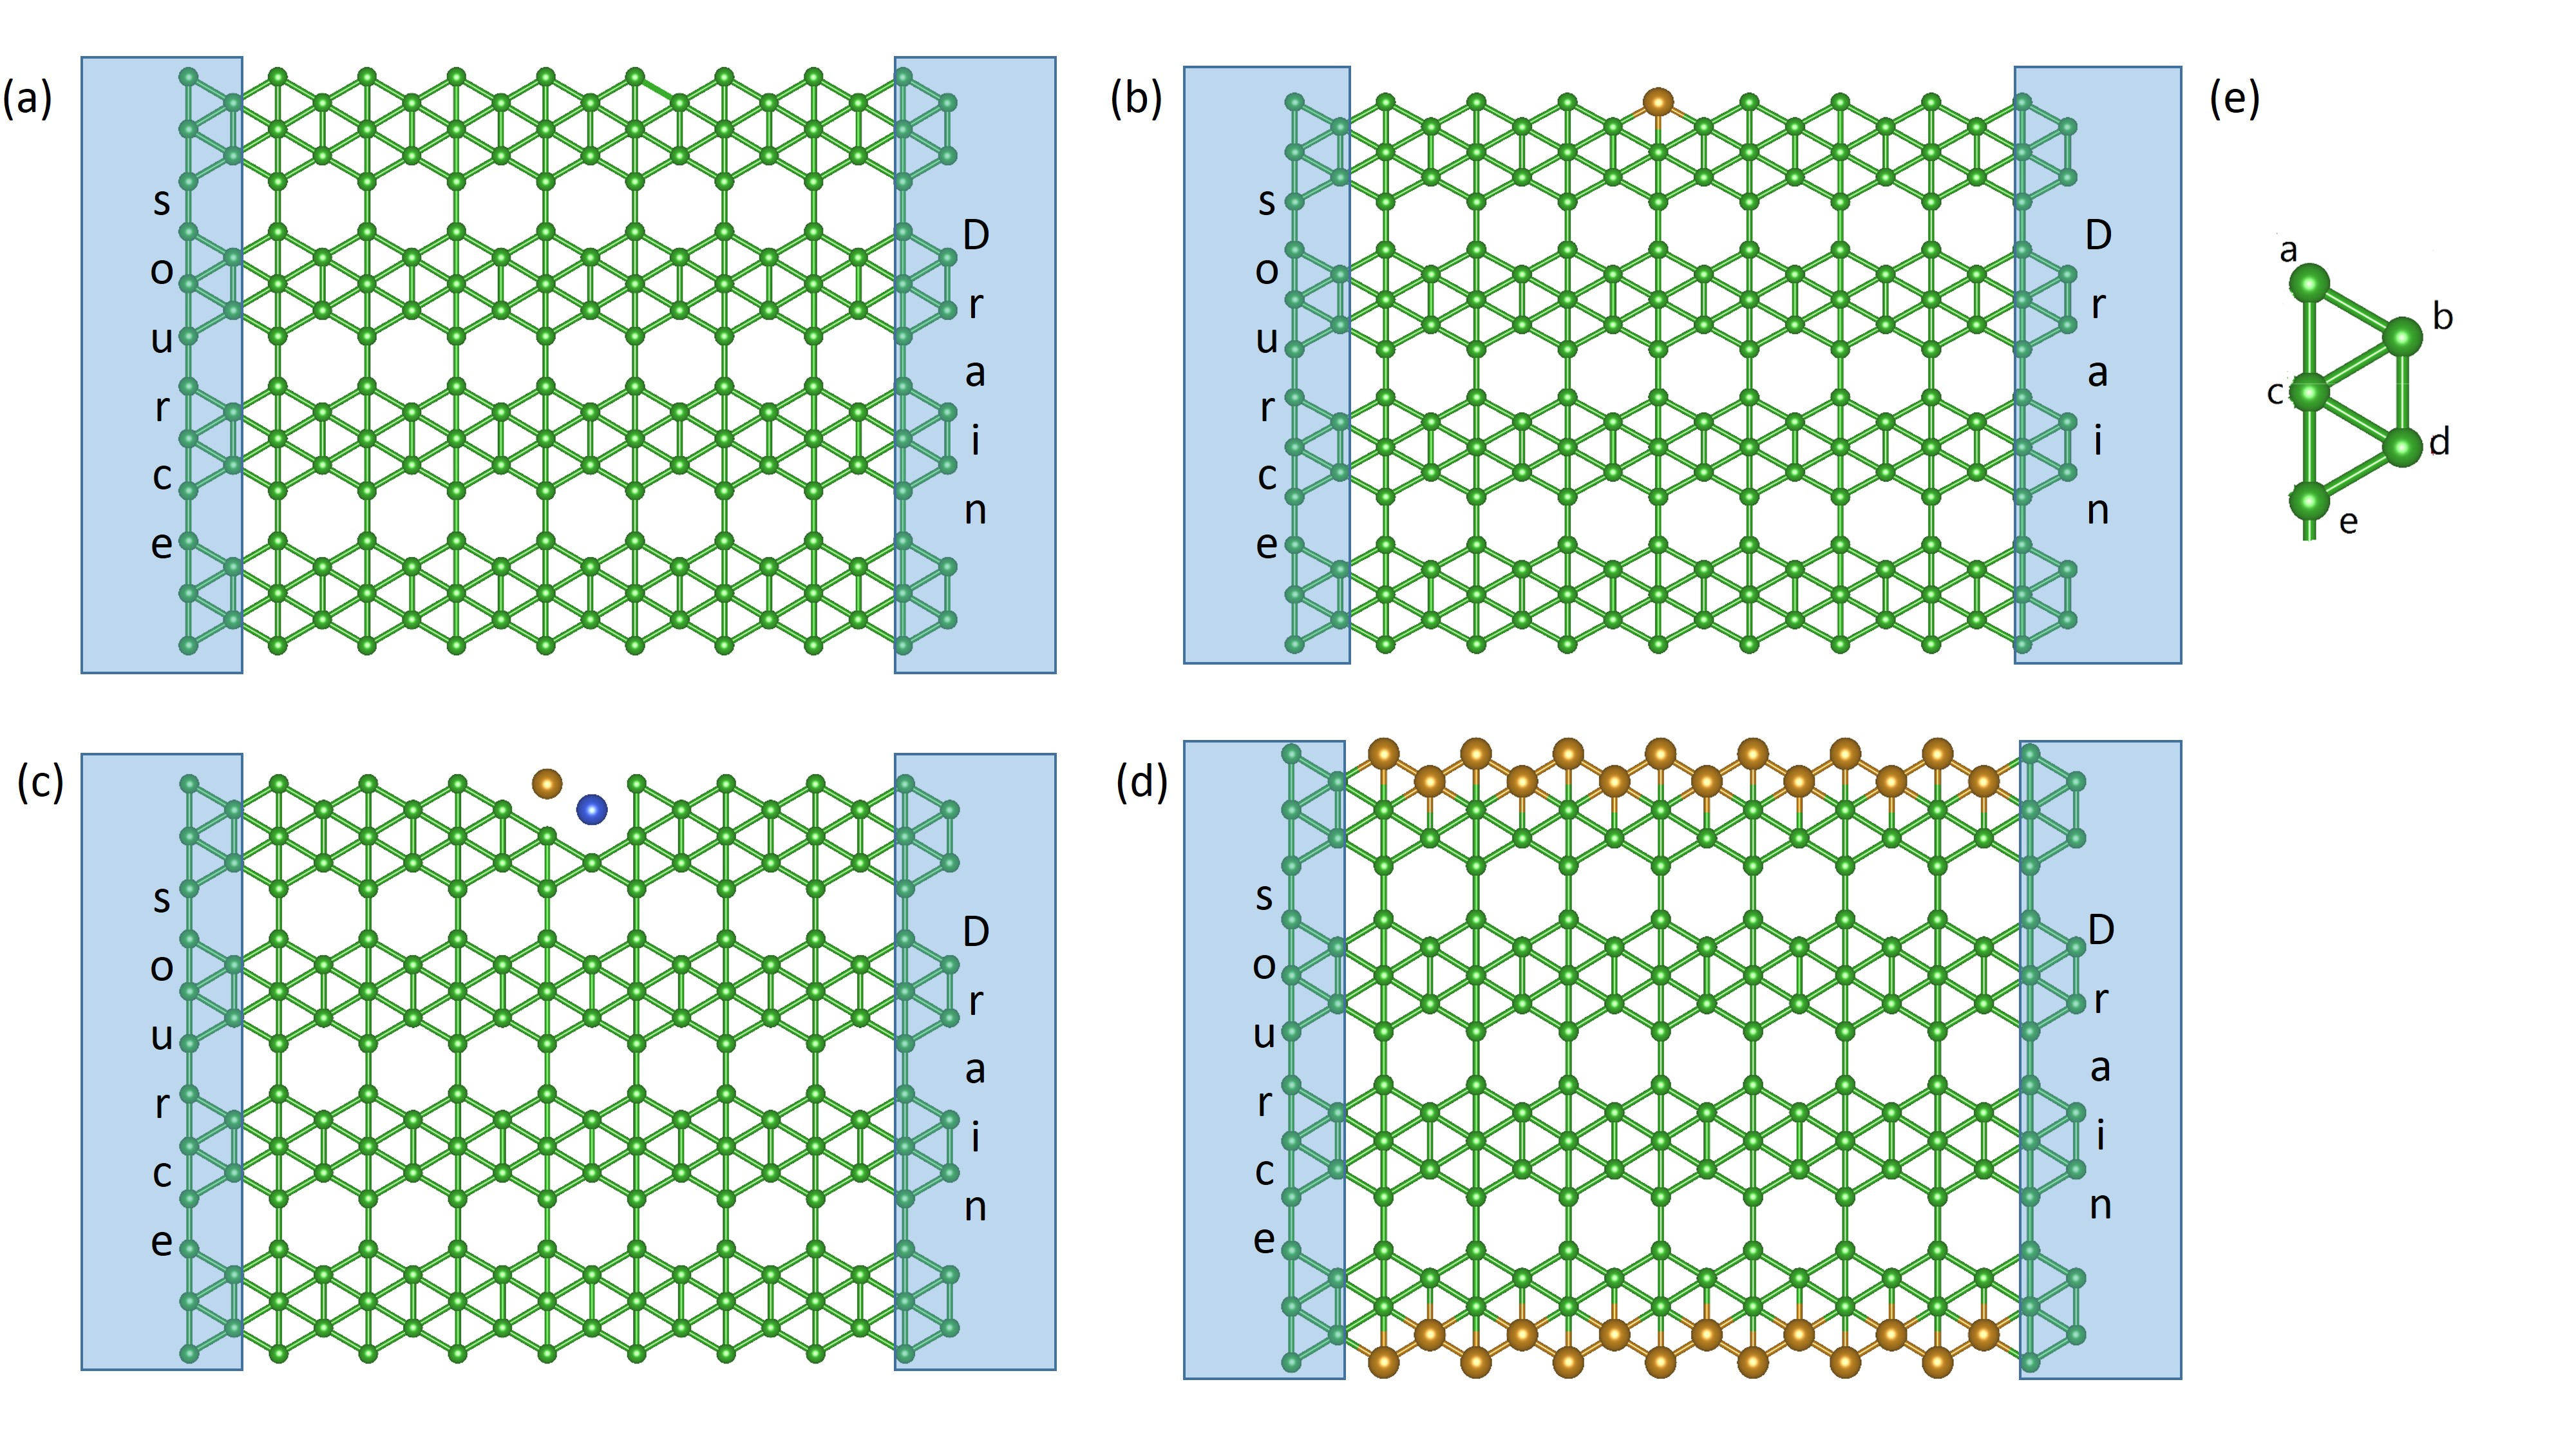
\includegraphics[width=1\linewidth]{./figures/borophene_structure(3).JPG}
    \caption{(الف) شماتیک نانوروبان زیگزاگ $\beta_{12}$-بوروفن که این ساختار از یک شبکه مربعی با پایه تشکیل شده است.(ب) شماتیک یک نانوروبان زیگزاگ $\beta_{12}$-بوروفن با ناخالصی لبه پراکنده.(ج) نمودار یک نانوروبان زیگزاگ $\beta_{12}$-بوروفن با یک و دو جای خالی در لبه.(د) شماتیک نانوروبان زیگزاگ $\beta_{12}$-بوروفن با اختلال لبه اندرسون.(ه) اساس شامل پنج اتم است که با a، b، c، d و e نشان داده می شوند.}
   \label{borophene}
\end{figure*}
  \begin{figure}[!ht]
    \centering
    % GNUPLOT: LaTeX picture with Postscript
\begingroup
  % Encoding inside the plot.  In the header of your document, this encoding
  % should to defined, e.g., by using
  % \usepackage[cp1252,<other encodings>]{inputenc}
  % \inputencoding{cp1252}%
  \makeatletter
  \providecommand\color[2][]{%
    \GenericError{(gnuplot) \space\space\space\@spaces}{%
      Package color not loaded in conjunction with
      terminal option `colourtext'%
    }{See the gnuplot documentation for explanation.%
    }{Either use 'blacktext' in gnuplot or load the package
      color.sty in LaTeX.}%
    \renewcommand\color[2][]{}%
  }%
  \providecommand\includegraphics[2][]{%
    \GenericError{(gnuplot) \space\space\space\@spaces}{%
      Package graphicx or graphics not loaded%
    }{See the gnuplot documentation for explanation.%
    }{The gnuplot epslatex terminal needs graphicx.sty or graphics.sty.}%
    \renewcommand\includegraphics[2][]{}%
  }%
  \providecommand\rotatebox[2]{#2}%
  \@ifundefined{ifGPcolor}{%
    \newif\ifGPcolor
    \GPcolorfalse
  }{}%
  \@ifundefined{ifGPblacktext}{%
    \newif\ifGPblacktext
    \GPblacktexttrue
  }{}%
  % define a \g@addto@macro without @ in the name:
  \let\gplgaddtomacro\g@addto@macro
  % define empty templates for all commands taking text:
  \gdef\gplbacktext{}%
  \gdef\gplfronttext{}%
  \makeatother
  \ifGPblacktext
    % no textcolor at all
    \def\colorrgb#1{}%
    \def\colorgray#1{}%
  \else
    % gray or color?
    \ifGPcolor
      \def\colorrgb#1{\color[rgb]{#1}}%
      \def\colorgray#1{\color[gray]{#1}}%
      \expandafter\def\csname LTw\endcsname{\color{white}}%
      \expandafter\def\csname LTb\endcsname{\color{black}}%
      \expandafter\def\csname LTa\endcsname{\color{black}}%
      \expandafter\def\csname LT0\endcsname{\color[rgb]{1,0,0}}%
      \expandafter\def\csname LT1\endcsname{\color[rgb]{0,1,0}}%
      \expandafter\def\csname LT2\endcsname{\color[rgb]{0,0,1}}%
      \expandafter\def\csname LT3\endcsname{\color[rgb]{1,0,1}}%
      \expandafter\def\csname LT4\endcsname{\color[rgb]{0,1,1}}%
      \expandafter\def\csname LT5\endcsname{\color[rgb]{1,1,0}}%
      \expandafter\def\csname LT6\endcsname{\color[rgb]{0,0,0}}%
      \expandafter\def\csname LT7\endcsname{\color[rgb]{1,0.3,0}}%
      \expandafter\def\csname LT8\endcsname{\color[rgb]{0.5,0.5,0.5}}%
    \else
      % gray
      \def\colorrgb#1{\color{black}}%
      \def\colorgray#1{\color[gray]{#1}}%
      \expandafter\def\csname LTw\endcsname{\color{white}}%
      \expandafter\def\csname LTb\endcsname{\color{black}}%
      \expandafter\def\csname LTa\endcsname{\color{black}}%
      \expandafter\def\csname LT0\endcsname{\color{black}}%
      \expandafter\def\csname LT1\endcsname{\color{black}}%
      \expandafter\def\csname LT2\endcsname{\color{black}}%
      \expandafter\def\csname LT3\endcsname{\color{black}}%
      \expandafter\def\csname LT4\endcsname{\color{black}}%
      \expandafter\def\csname LT5\endcsname{\color{black}}%
      \expandafter\def\csname LT6\endcsname{\color{black}}%
      \expandafter\def\csname LT7\endcsname{\color{black}}%
      \expandafter\def\csname LT8\endcsname{\color{black}}%
    \fi
  \fi
    \setlength{\unitlength}{0.0500bp}%
    \ifx\gptboxheight\undefined%
      \newlength{\gptboxheight}%
      \newlength{\gptboxwidth}%
      \newsavebox{\gptboxtext}%
    \fi%
    \setlength{\fboxrule}{0.5pt}%
    \setlength{\fboxsep}{1pt}%
\begin{picture}(4320.00,5760.00)%
    \gplgaddtomacro\gplbacktext{%
      \csname LTb\endcsname%%
      \put(300,3320){\makebox(0,0)[r]{\strut{}$0$}}%
      \put(300,3567){\makebox(0,0)[r]{\strut{}$1$}}%
      \put(300,3813){\makebox(0,0)[r]{\strut{}$2$}}%
      \put(300,4060){\makebox(0,0)[r]{\strut{}$3$}}%
      \put(300,4306){\makebox(0,0)[r]{\strut{}$4$}}%
      \put(300,4553){\makebox(0,0)[r]{\strut{}$5$}}%
      \put(300,4799){\makebox(0,0)[r]{\strut{}$6$}}%
      \put(300,5046){\makebox(0,0)[r]{\strut{}$7$}}%
      \put(300,5292){\makebox(0,0)[r]{\strut{}$8$}}%
      \put(300,5539){\makebox(0,0)[r]{\strut{}$9$}}%
      \put(432,3100){\makebox(0,0){\strut{}$-2$}}%
      \put(866,3100){\makebox(0,0){\strut{}$-1.5$}}%
      \put(1300,3100){\makebox(0,0){\strut{}$-1$}}%
      \put(1735,3100){\makebox(0,0){\strut{}$-0.5$}}%
      \put(2169,3100){\makebox(0,0){\strut{}$0$}}%
      \put(2603,3100){\makebox(0,0){\strut{}$0.5$}}%
      \put(3037,3100){\makebox(0,0){\strut{}$1$}}%
      \put(3471,3100){\makebox(0,0){\strut{}$1.5$}}%
      \put(3906,3100){\makebox(0,0){\strut{}$2$}}%
      \put(607,5428){\makebox(0,0)[l]{\strut{}(a)}}%
    }%
    \gplgaddtomacro\gplfronttext{%
      \csname LTb\endcsname%%
      \put(-52,4429){\rotatebox{-270}{\makebox(0,0){\strut{}$G/G_0$}}}%
      \csname LTb\endcsname%%
      \put(2936,5366){\makebox(0,0)[r]{\strut{}Pristine-$\beta_{12}$}}%
      \csname LTb\endcsname%%
      \put(2936,5146){\makebox(0,0)[r]{\strut{}V=1 eV}}%
      \csname LTb\endcsname%%
      \put(2936,4926){\makebox(0,0)[r]{\strut{}V=2 eV}}%
      \csname LTb\endcsname%%
      \put(2936,4706){\makebox(0,0)[r]{\strut{}V=5 eV}}%
    }%
    \gplgaddtomacro\gplbacktext{%
      \csname LTb\endcsname%%
      \put(300,704){\makebox(0,0)[r]{\strut{}$0$}}%
      \put(300,1193){\makebox(0,0)[r]{\strut{}$0.05$}}%
      \put(300,1682){\makebox(0,0)[r]{\strut{}$0.1$}}%
      \put(300,2171){\makebox(0,0)[r]{\strut{}$0.15$}}%
      \put(300,2660){\makebox(0,0)[r]{\strut{}$0.2$}}%
      \put(432,484){\makebox(0,0){\strut{}$-2$}}%
      \put(866,484){\makebox(0,0){\strut{}$-1.5$}}%
      \put(1300,484){\makebox(0,0){\strut{}$-1$}}%
      \put(1735,484){\makebox(0,0){\strut{}$-0.5$}}%
      \put(2169,484){\makebox(0,0){\strut{}$0$}}%
      \put(2603,484){\makebox(0,0){\strut{}$0.5$}}%
      \put(3037,484){\makebox(0,0){\strut{}$1$}}%
      \put(3471,484){\makebox(0,0){\strut{}$1.5$}}%
      \put(3906,484){\makebox(0,0){\strut{}$2$}}%
      \put(607,2562){\makebox(0,0)[l]{\strut{}(b)}}%
    }%
    \gplgaddtomacro\gplfronttext{%
      \csname LTb\endcsname%%
      \put(-448,1682){\rotatebox{-270}{\makebox(0,0){\strut{}LDOS}}}%
      \put(2177,154){\makebox(0,0){\strut{}Energy(eV)}}%
    }%
    \gplbacktext
    \put(0,0){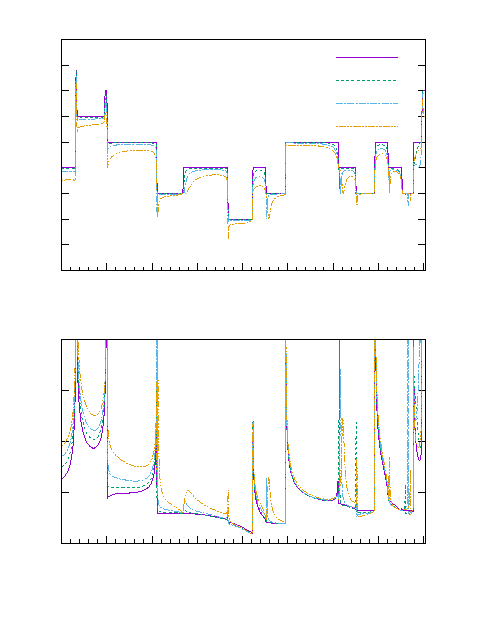
\includegraphics[width={217.00bp},height={289.00bp}]{zigscatter}}%
    \gplfronttext
  \end{picture}%
\endgroup

    \caption{الف) رسانایی نانو نوارهای زیگزاگی با عرض $18.59$\AA و طول $42.34$\AA، با ناخالصی واقع در لبه بالایی یک سوپرسل در نانو نوار. (ب) چگالی الکترونی حالات در نزدیکترین محل همسایه ناخالصی که همان a.}
    \label{zigscatter}
  \end{figure}
  \begin{figure}[ht]
    \centering
    % GNUPLOT: LaTeX picture with Postscript
\begingroup
  % Encoding inside the plot.  In the header of your document, this encoding
  % should to defined, e.g., by using
  % \usepackage[cp1252,<other encodings>]{inputenc}
  % \inputencoding{cp1252}%
  \makeatletter
  \providecommand\color[2][]{%
    \GenericError{(gnuplot) \space\space\space\@spaces}{%
      Package color not loaded in conjunction with
      terminal option `colourtext'%
    }{See the gnuplot documentation for explanation.%
    }{Either use 'blacktext' in gnuplot or load the package
      color.sty in LaTeX.}%
    \renewcommand\color[2][]{}%
  }%
  \providecommand\includegraphics[2][]{%
    \GenericError{(gnuplot) \space\space\space\@spaces}{%
      Package graphicx or graphics not loaded%
    }{See the gnuplot documentation for explanation.%
    }{The gnuplot epslatex terminal needs graphicx.sty or graphics.sty.}%
    \renewcommand\includegraphics[2][]{}%
  }%
  \providecommand\rotatebox[2]{#2}%
  \@ifundefined{ifGPcolor}{%
    \newif\ifGPcolor
    \GPcolorfalse
  }{}%
  \@ifundefined{ifGPblacktext}{%
    \newif\ifGPblacktext
    \GPblacktexttrue
  }{}%
  % define a \g@addto@macro without @ in the name:
  \let\gplgaddtomacro\g@addto@macro
  % define empty templates for all commands taking text:
  \gdef\gplbacktext{}%
  \gdef\gplfronttext{}%
  \makeatother
  \ifGPblacktext
    % no textcolor at all
    \def\colorrgb#1{}%
    \def\colorgray#1{}%
  \else
    % gray or color?
    \ifGPcolor
      \def\colorrgb#1{\color[rgb]{#1}}%
      \def\colorgray#1{\color[gray]{#1}}%
      \expandafter\def\csname LTw\endcsname{\color{white}}%
      \expandafter\def\csname LTb\endcsname{\color{black}}%
      \expandafter\def\csname LTa\endcsname{\color{black}}%
      \expandafter\def\csname LT0\endcsname{\color[rgb]{1,0,0}}%
      \expandafter\def\csname LT1\endcsname{\color[rgb]{0,1,0}}%
      \expandafter\def\csname LT2\endcsname{\color[rgb]{0,0,1}}%
      \expandafter\def\csname LT3\endcsname{\color[rgb]{1,0,1}}%
      \expandafter\def\csname LT4\endcsname{\color[rgb]{0,1,1}}%
      \expandafter\def\csname LT5\endcsname{\color[rgb]{1,1,0}}%
      \expandafter\def\csname LT6\endcsname{\color[rgb]{0,0,0}}%
      \expandafter\def\csname LT7\endcsname{\color[rgb]{1,0.3,0}}%
      \expandafter\def\csname LT8\endcsname{\color[rgb]{0.5,0.5,0.5}}%
    \else
      % gray
      \def\colorrgb#1{\color{black}}%
      \def\colorgray#1{\color[gray]{#1}}%
      \expandafter\def\csname LTw\endcsname{\color{white}}%
      \expandafter\def\csname LTb\endcsname{\color{black}}%
      \expandafter\def\csname LTa\endcsname{\color{black}}%
      \expandafter\def\csname LT0\endcsname{\color{black}}%
      \expandafter\def\csname LT1\endcsname{\color{black}}%
      \expandafter\def\csname LT2\endcsname{\color{black}}%
      \expandafter\def\csname LT3\endcsname{\color{black}}%
      \expandafter\def\csname LT4\endcsname{\color{black}}%
      \expandafter\def\csname LT5\endcsname{\color{black}}%
      \expandafter\def\csname LT6\endcsname{\color{black}}%
      \expandafter\def\csname LT7\endcsname{\color{black}}%
      \expandafter\def\csname LT8\endcsname{\color{black}}%
    \fi
  \fi
    \setlength{\unitlength}{0.0500bp}%
    \ifx\gptboxheight\undefined%
      \newlength{\gptboxheight}%
      \newlength{\gptboxwidth}%
      \newsavebox{\gptboxtext}%
    \fi%
    \setlength{\fboxrule}{0.5pt}%
    \setlength{\fboxsep}{1pt}%
\begin{picture}(4320.00,5760.00)%
    \gplgaddtomacro\gplbacktext{%
      \csname LTb\endcsname%%
      \put(300,3320){\makebox(0,0)[r]{\strut{}$0$}}%
      \put(300,3597){\makebox(0,0)[r]{\strut{}$1$}}%
      \put(300,3875){\makebox(0,0)[r]{\strut{}$2$}}%
      \put(300,4152){\makebox(0,0)[r]{\strut{}$3$}}%
      \put(300,4430){\makebox(0,0)[r]{\strut{}$4$}}%
      \put(300,4707){\makebox(0,0)[r]{\strut{}$5$}}%
      \put(300,4984){\makebox(0,0)[r]{\strut{}$6$}}%
      \put(300,5262){\makebox(0,0)[r]{\strut{}$7$}}%
      \put(300,5539){\makebox(0,0)[r]{\strut{}$8$}}%
      \put(432,3100){\makebox(0,0){\strut{}$-2$}}%
      \put(868,3100){\makebox(0,0){\strut{}$-1.5$}}%
      \put(1305,3100){\makebox(0,0){\strut{}$-1$}}%
      \put(1741,3100){\makebox(0,0){\strut{}$-0.5$}}%
      \put(2178,3100){\makebox(0,0){\strut{}$0$}}%
      \put(2614,3100){\makebox(0,0){\strut{}$0.5$}}%
      \put(3050,3100){\makebox(0,0){\strut{}$1$}}%
      \put(3487,3100){\makebox(0,0){\strut{}$1.5$}}%
      \put(3923,3100){\makebox(0,0){\strut{}$2$}}%
      \put(676,5428){\makebox(0,0)[l]{\strut{}(a)}}%
    }%
    \gplgaddtomacro\gplfronttext{%
      \csname LTb\endcsname%%
      \put(-52,4429){\rotatebox{-270}{\makebox(0,0){\strut{}$G/G_0$}}}%
      \csname LTb\endcsname%%
      \put(2936,5366){\makebox(0,0)[r]{\strut{}Pristine-$\beta_{12}$}}%
      \csname LTb\endcsname%%
      \put(2936,5146){\makebox(0,0)[r]{\strut{}V=1 eV}}%
      \csname LTb\endcsname%%
      \put(2936,4926){\makebox(0,0)[r]{\strut{}V=2 eV}}%
      \csname LTb\endcsname%%
      \put(2936,4706){\makebox(0,0)[r]{\strut{}V=5 eV}}%
    }%
    \gplgaddtomacro\gplbacktext{%
      \csname LTb\endcsname%%
      \put(300,704){\makebox(0,0)[r]{\strut{}$0$}}%
      \put(300,1095){\makebox(0,0)[r]{\strut{}$0.1$}}%
      \put(300,1486){\makebox(0,0)[r]{\strut{}$0.2$}}%
      \put(300,1878){\makebox(0,0)[r]{\strut{}$0.3$}}%
      \put(300,2269){\makebox(0,0)[r]{\strut{}$0.4$}}%
      \put(300,2660){\makebox(0,0)[r]{\strut{}$0.5$}}%
      \put(432,484){\makebox(0,0){\strut{}$-2$}}%
      \put(868,484){\makebox(0,0){\strut{}$-1.5$}}%
      \put(1305,484){\makebox(0,0){\strut{}$-1$}}%
      \put(1741,484){\makebox(0,0){\strut{}$-0.5$}}%
      \put(2178,484){\makebox(0,0){\strut{}$0$}}%
      \put(2614,484){\makebox(0,0){\strut{}$0.5$}}%
      \put(3050,484){\makebox(0,0){\strut{}$1$}}%
      \put(3487,484){\makebox(0,0){\strut{}$1.5$}}%
      \put(3923,484){\makebox(0,0){\strut{}$2$}}%
      \put(676,2562){\makebox(0,0)[l]{\strut{}(b)}}%
    }%
    \gplgaddtomacro\gplfronttext{%
      \csname LTb\endcsname%%
      \put(-316,1682){\rotatebox{-270}{\makebox(0,0){\strut{}LDOS}}}%
      \put(2177,154){\makebox(0,0){\strut{}Energy(eV)}}%
    }%
    \gplbacktext
    \put(0,0){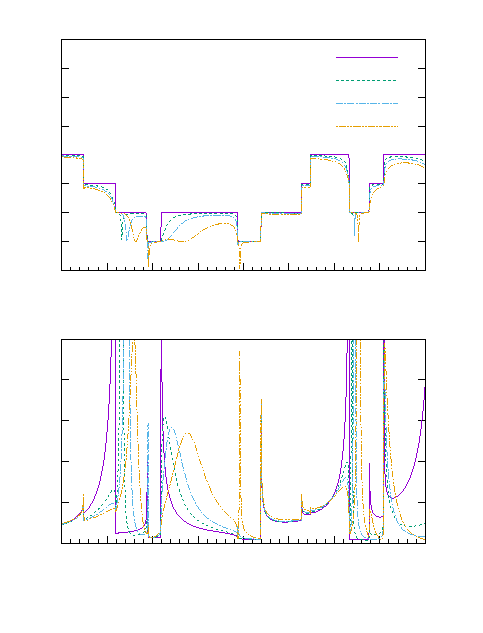
\includegraphics[width={217.00bp},height={289.00bp}]{armscatter}}%
    \gplfronttext
  \end{picture}%
\endgroup

    \caption{(الف) رسانایی نانو نوارهای صندلی صندلی با عرض $10.24$\AA و طول $74.36$\AA با ناخالصی واقع در لبه بالایی یک سوپرسل در نانو نوار. (ب) چگالی الکترونی حالات در نزدیکترین محل همسایه ناخالصی که همان a.}
    \label{armscatter}
  \end{figure}

در میان مراحل مختلف پیشنهاد شده برای بوروفن [20-23]، $\beta_{12}$  پایدارترین تک لایه بور [24]. $\beta_{12}$ نیز نسبت به سایر آلوتروپ های خود در برابر اکسیداسیون بی اثرتر است، که مزیت خوبی برای کاربرد دستگاه ها در آینده است [16].

\begin{figure}[ht]
    \centering
    % GNUPLOT: LaTeX picture with Postscript
\begingroup
  % Encoding inside the plot.  In the header of your document, this encoding
  % should to defined, e.g., by using
  % \usepackage[cp1252,<other encodings>]{inputenc}
  % \inputencoding{cp1252}%
  \makeatletter
  \providecommand\color[2][]{%
    \GenericError{(gnuplot) \space\space\space\@spaces}{%
      Package color not loaded in conjunction with
      terminal option `colourtext'%
    }{See the gnuplot documentation for explanation.%
    }{Either use 'blacktext' in gnuplot or load the package
      color.sty in LaTeX.}%
    \renewcommand\color[2][]{}%
  }%
  \providecommand\includegraphics[2][]{%
    \GenericError{(gnuplot) \space\space\space\@spaces}{%
      Package graphicx or graphics not loaded%
    }{See the gnuplot documentation for explanation.%
    }{The gnuplot epslatex terminal needs graphicx.sty or graphics.sty.}%
    \renewcommand\includegraphics[2][]{}%
  }%
  \providecommand\rotatebox[2]{#2}%
  \@ifundefined{ifGPcolor}{%
    \newif\ifGPcolor
    \GPcolorfalse
  }{}%
  \@ifundefined{ifGPblacktext}{%
    \newif\ifGPblacktext
    \GPblacktexttrue
  }{}%
  % define a \g@addto@macro without @ in the name:
  \let\gplgaddtomacro\g@addto@macro
  % define empty templates for all commands taking text:
  \gdef\gplbacktext{}%
  \gdef\gplfronttext{}%
  \makeatother
  \ifGPblacktext
    % no textcolor at all
    \def\colorrgb#1{}%
    \def\colorgray#1{}%
  \else
    % gray or color?
    \ifGPcolor
      \def\colorrgb#1{\color[rgb]{#1}}%
      \def\colorgray#1{\color[gray]{#1}}%
      \expandafter\def\csname LTw\endcsname{\color{white}}%
      \expandafter\def\csname LTb\endcsname{\color{black}}%
      \expandafter\def\csname LTa\endcsname{\color{black}}%
      \expandafter\def\csname LT0\endcsname{\color[rgb]{1,0,0}}%
      \expandafter\def\csname LT1\endcsname{\color[rgb]{0,1,0}}%
      \expandafter\def\csname LT2\endcsname{\color[rgb]{0,0,1}}%
      \expandafter\def\csname LT3\endcsname{\color[rgb]{1,0,1}}%
      \expandafter\def\csname LT4\endcsname{\color[rgb]{0,1,1}}%
      \expandafter\def\csname LT5\endcsname{\color[rgb]{1,1,0}}%
      \expandafter\def\csname LT6\endcsname{\color[rgb]{0,0,0}}%
      \expandafter\def\csname LT7\endcsname{\color[rgb]{1,0.3,0}}%
      \expandafter\def\csname LT8\endcsname{\color[rgb]{0.5,0.5,0.5}}%
    \else
      % gray
      \def\colorrgb#1{\color{black}}%
      \def\colorgray#1{\color[gray]{#1}}%
      \expandafter\def\csname LTw\endcsname{\color{white}}%
      \expandafter\def\csname LTb\endcsname{\color{black}}%
      \expandafter\def\csname LTa\endcsname{\color{black}}%
      \expandafter\def\csname LT0\endcsname{\color{black}}%
      \expandafter\def\csname LT1\endcsname{\color{black}}%
      \expandafter\def\csname LT2\endcsname{\color{black}}%
      \expandafter\def\csname LT3\endcsname{\color{black}}%
      \expandafter\def\csname LT4\endcsname{\color{black}}%
      \expandafter\def\csname LT5\endcsname{\color{black}}%
      \expandafter\def\csname LT6\endcsname{\color{black}}%
      \expandafter\def\csname LT7\endcsname{\color{black}}%
      \expandafter\def\csname LT8\endcsname{\color{black}}%
    \fi
  \fi
    \setlength{\unitlength}{0.0500bp}%
    \ifx\gptboxheight\undefined%
      \newlength{\gptboxheight}%
      \newlength{\gptboxwidth}%
      \newsavebox{\gptboxtext}%
    \fi%
    \setlength{\fboxrule}{0.5pt}%
    \setlength{\fboxsep}{1pt}%
\begin{picture}(4320.00,5760.00)%
    \gplgaddtomacro\gplbacktext{%
      \csname LTb\endcsname%%
      \put(300,3320){\makebox(0,0)[r]{\strut{}$0$}}%
      \put(300,3597){\makebox(0,0)[r]{\strut{}$1$}}%
      \put(300,3875){\makebox(0,0)[r]{\strut{}$2$}}%
      \put(300,4152){\makebox(0,0)[r]{\strut{}$3$}}%
      \put(300,4430){\makebox(0,0)[r]{\strut{}$4$}}%
      \put(300,4707){\makebox(0,0)[r]{\strut{}$5$}}%
      \put(300,4984){\makebox(0,0)[r]{\strut{}$6$}}%
      \put(300,5262){\makebox(0,0)[r]{\strut{}$7$}}%
      \put(300,5539){\makebox(0,0)[r]{\strut{}$8$}}%
      \put(432,3100){\makebox(0,0){\strut{}$-2$}}%
      \put(866,3100){\makebox(0,0){\strut{}$-1.5$}}%
      \put(1300,3100){\makebox(0,0){\strut{}$-1$}}%
      \put(1735,3100){\makebox(0,0){\strut{}$-0.5$}}%
      \put(2169,3100){\makebox(0,0){\strut{}$0$}}%
      \put(2603,3100){\makebox(0,0){\strut{}$0.5$}}%
      \put(3037,3100){\makebox(0,0){\strut{}$1$}}%
      \put(3471,3100){\makebox(0,0){\strut{}$1.5$}}%
      \put(3906,3100){\makebox(0,0){\strut{}$2$}}%
      \put(676,5428){\makebox(0,0)[l]{\strut{}(a)}}%
    }%
    \gplgaddtomacro\gplfronttext{%
      \csname LTb\endcsname%%
      \put(-52,4429){\rotatebox{-270}{\makebox(0,0){\strut{}$G/G_0$}}}%
      \csname LTb\endcsname%%
      \put(2936,5366){\makebox(0,0)[r]{\strut{}Pristine-$\beta_{12}$}}%
      \csname LTb\endcsname%%
      \put(2936,5146){\makebox(0,0)[r]{\strut{}One edge Vacancy}}%
      \csname LTb\endcsname%%
      \put(2936,4926){\makebox(0,0)[r]{\strut{}Two edges Vacancies}}%
    }%
    \gplgaddtomacro\gplbacktext{%
      \csname LTb\endcsname%%
      \put(300,704){\makebox(0,0)[r]{\strut{}$0$}}%
      \put(300,1095){\makebox(0,0)[r]{\strut{}$0.1$}}%
      \put(300,1486){\makebox(0,0)[r]{\strut{}$0.2$}}%
      \put(300,1878){\makebox(0,0)[r]{\strut{}$0.3$}}%
      \put(300,2269){\makebox(0,0)[r]{\strut{}$0.4$}}%
      \put(300,2660){\makebox(0,0)[r]{\strut{}$0.5$}}%
      \put(432,484){\makebox(0,0){\strut{}$-2$}}%
      \put(868,484){\makebox(0,0){\strut{}$-1.5$}}%
      \put(1305,484){\makebox(0,0){\strut{}$-1$}}%
      \put(1741,484){\makebox(0,0){\strut{}$-0.5$}}%
      \put(2178,484){\makebox(0,0){\strut{}$0$}}%
      \put(2614,484){\makebox(0,0){\strut{}$0.5$}}%
      \put(3050,484){\makebox(0,0){\strut{}$1$}}%
      \put(3487,484){\makebox(0,0){\strut{}$1.5$}}%
      \put(3923,484){\makebox(0,0){\strut{}$2$}}%
      \put(676,2562){\makebox(0,0)[l]{\strut{}(b)}}%
    }%
    \gplgaddtomacro\gplfronttext{%
      \csname LTb\endcsname%%
      \put(-316,1682){\rotatebox{-270}{\makebox(0,0){\strut{}LDOS}}}%
      \put(2177,154){\makebox(0,0){\strut{}Energy(eV)}}%
    }%
    \gplbacktext
    \put(0,0){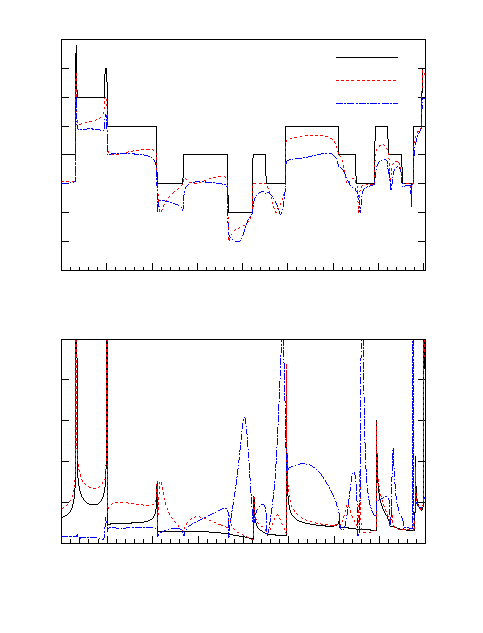
\includegraphics[width={217.00bp},height={289.00bp}]{zigvacancy}}%
    \gplfronttext
  \end{picture}%
\endgroup

    \caption{(الف) رسانایی نانو نوارهای زیگزاگی با a
    عرض $18.59$\AA و طول $42.34$\AA، با جاهای خالی در لبه بالایی سوپرسل میانی قرار دارد.(ب) چگالی الکترونی حالات در نزدیکترین محل همسایه جاهای خالی واقع در همان (a).}
    \label{armvacancy}
  \end{figure}
  
\begin{figure}[ht]
\centering
% GNUPLOT: LaTeX picture with Postscript
\begin{latin}
\begingroup
  \makeatletter
  \providecommand\color[2][]{%
    \GenericError{(gnuplot) \space\space\space\@spaces}{%
      Package color not loaded in conjunction with
      terminal option `colourtext'%
    }{See the gnuplot documentation for explanation.%
    }{Either use 'blacktext' in gnuplot or load the package
      color.sty in LaTeX.}%
    \renewcommand\color[2][]{}%
  }%
  \providecommand\includegraphics[2][]{%
    \GenericError{(gnuplot) \space\space\space\@spaces}{%
      Package graphicx or graphics not loaded%
    }{See the gnuplot documentation for explanation.%
    }{The gnuplot epslatex terminal needs graphicx.sty or graphics.sty.}%
    \renewcommand\includegraphics[2][]{}%
  }%
  \providecommand\rotatebox[2]{#2}%
  \@ifundefined{ifGPcolor}{%
    \newif\ifGPcolor
    \GPcolorfalse
  }{}%
  \@ifundefined{ifGPblacktext}{%
    \newif\ifGPblacktext
    \GPblacktexttrue
  }{}%
  % define a \g@addto@macro without @ in the name:
  \let\gplgaddtomacro\g@addto@macro
  % define empty templates for all commands taking text:
  \gdef\gplbacktext{}%
  \gdef\gplfronttext{}%
  \makeatother
  \ifGPblacktext
    % no textcolor at all
    \def\colorrgb#1{}%
    \def\colorgray#1{}%
  \else
    % gray or color?
    \ifGPcolor
      \def\colorrgb#1{\color[rgb]{#1}}%
      \def\colorgray#1{\color[gray]{#1}}%
      \expandafter\def\csname LTw\endcsname{\color{white}}%
      \expandafter\def\csname LTb\endcsname{\color{black}}%
      \expandafter\def\csname LTa\endcsname{\color{black}}%
      \expandafter\def\csname LT0\endcsname{\color[rgb]{1,0,0}}%
      \expandafter\def\csname LT1\endcsname{\color[rgb]{0,1,0}}%
      \expandafter\def\csname LT2\endcsname{\color[rgb]{0,0,1}}%
      \expandafter\def\csname LT3\endcsname{\color[rgb]{1,0,1}}%
      \expandafter\def\csname LT4\endcsname{\color[rgb]{0,1,1}}%
      \expandafter\def\csname LT5\endcsname{\color[rgb]{1,1,0}}%
      \expandafter\def\csname LT6\endcsname{\color[rgb]{0,0,0}}%
      \expandafter\def\csname LT7\endcsname{\color[rgb]{1,0.3,0}}%
      \expandafter\def\csname LT8\endcsname{\color[rgb]{0.5,0.5,0.5}}%
    \else
      % gray
      \def\colorrgb#1{\color{black}}%
      \def\colorgray#1{\color[gray]{#1}}%
      \expandafter\def\csname LTw\endcsname{\color{white}}%
      \expandafter\def\csname LTb\endcsname{\color{black}}%
      \expandafter\def\csname LTa\endcsname{\color{black}}%
      \expandafter\def\csname LT0\endcsname{\color{black}}%
      \expandafter\def\csname LT1\endcsname{\color{black}}%
      \expandafter\def\csname LT2\endcsname{\color{black}}%
      \expandafter\def\csname LT3\endcsname{\color{black}}%
      \expandafter\def\csname LT4\endcsname{\color{black}}%
      \expandafter\def\csname LT5\endcsname{\color{black}}%
      \expandafter\def\csname LT6\endcsname{\color{black}}%
      \expandafter\def\csname LT7\endcsname{\color{black}}%
      \expandafter\def\csname LT8\endcsname{\color{black}}%
    \fi
  \fi
    \setlength{\unitlength}{0.0500bp}%
    \ifx\gptboxheight\undefined%
      \newlength{\gptboxheight}%
      \newlength{\gptboxwidth}%
      \newsavebox{\gptboxtext}%
    \fi%
    \setlength{\fboxrule}{0.5pt}%
    \setlength{\fboxsep}{1pt}%
\begin{picture}(4320.00,5760.00)%
    \gplgaddtomacro\gplbacktext{%
      \csname LTb\endcsname%%
      \put(300,3320){\makebox(0,0)[r]{\strut{}$0$}}%
      \put(300,3597){\makebox(0,0)[r]{\strut{}$1$}}%
      \put(300,3875){\makebox(0,0)[r]{\strut{}$2$}}%
      \put(300,4152){\makebox(0,0)[r]{\strut{}$3$}}%
      \put(300,4430){\makebox(0,0)[r]{\strut{}$4$}}%
      \put(300,4707){\makebox(0,0)[r]{\strut{}$5$}}%
      \put(300,4984){\makebox(0,0)[r]{\strut{}$6$}}%
      \put(300,5262){\makebox(0,0)[r]{\strut{}$7$}}%
      \put(300,5539){\makebox(0,0)[r]{\strut{}$8$}}%
      \put(432,3100){\makebox(0,0){\strut{}$-2$}}%
      \put(868,3100){\makebox(0,0){\strut{}$-1.5$}}%
      \put(1305,3100){\makebox(0,0){\strut{}$-1$}}%
      \put(1741,3100){\makebox(0,0){\strut{}$-0.5$}}%
      \put(2178,3100){\makebox(0,0){\strut{}$0$}}%
      \put(2614,3100){\makebox(0,0){\strut{}$0.5$}}%
      \put(3050,3100){\makebox(0,0){\strut{}$1$}}%
      \put(3487,3100){\makebox(0,0){\strut{}$1.5$}}%
      \put(3923,3100){\makebox(0,0){\strut{}$2$}}%
      \put(711,5428){\makebox(0,0)[l]{\strut{}(a)}}%
    }%
    \gplgaddtomacro\gplfronttext{%
      \csname LTb\endcsname%%
      \put(-52,4429){\rotatebox{-270}{\makebox(0,0){\strut{}$G/G_0$}}}%
      \csname LTb\endcsname%%
      \put(2936,5366){\makebox(0,0)[r]{\strut{}Pristine-$\beta_{12}$}}%
      \csname LTb\endcsname%%
      \put(2936,5146){\makebox(0,0)[r]{\strut{}One edge Vacancy}}%
      \csname LTb\endcsname%%
      \put(2936,4926){\makebox(0,0)[r]{\strut{}Two edges Vacancies}}%
    }%
    \gplgaddtomacro\gplbacktext{%
      \csname LTb\endcsname%%
      \put(300,704){\makebox(0,0)[r]{\strut{}$0$}}%
      \put(300,1095){\makebox(0,0)[r]{\strut{}$0.2$}}%
      \put(300,1486){\makebox(0,0)[r]{\strut{}$0.4$}}%
      \put(300,1878){\makebox(0,0)[r]{\strut{}$0.6$}}%
      \put(300,2269){\makebox(0,0)[r]{\strut{}$0.8$}}%
      \put(300,2660){\makebox(0,0)[r]{\strut{}$1$}}%
      \put(432,484){\makebox(0,0){\strut{}$-2$}}%
      \put(868,484){\makebox(0,0){\strut{}$-1.5$}}%
      \put(1305,484){\makebox(0,0){\strut{}$-1$}}%
      \put(1741,484){\makebox(0,0){\strut{}$-0.5$}}%
      \put(2178,484){\makebox(0,0){\strut{}$0$}}%
      \put(2614,484){\makebox(0,0){\strut{}$0.5$}}%
      \put(3050,484){\makebox(0,0){\strut{}$1$}}%
      \put(3487,484){\makebox(0,0){\strut{}$1.5$}}%
      \put(3923,484){\makebox(0,0){\strut{}$2$}}%
      \put(711,2562){\makebox(0,0)[l]{\strut{}(b)}}%
    }%
    \gplgaddtomacro\gplfronttext{%
      \csname LTb\endcsname%%
      \put(-316,1682){\rotatebox{-270}{\makebox(0,0){\strut{}LDOS}}}%
      \put(2177,154){\makebox(0,0){\strut{}Energy(eV)}}%
    }%
    \gplbacktext
    \put(0,0){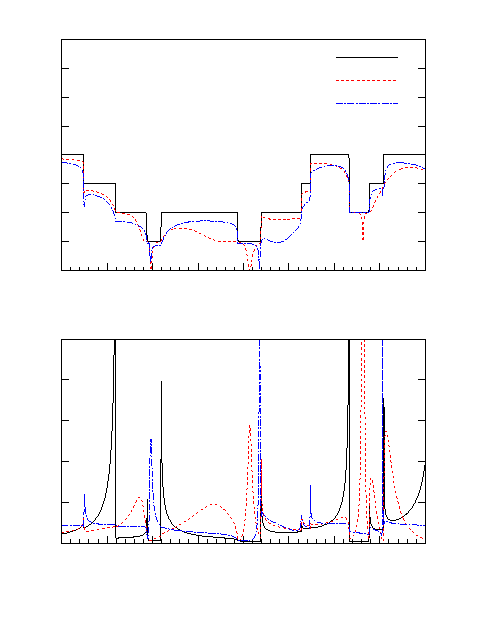
\includegraphics[width={217.00bp},height={289.00bp}]{armvacancy}}%
    \gplfronttext
  \end{picture}%
\endgroup
\end{latin}
\caption{(الف) رسانایی نانو نوارهای صندلی صندلی با a
عرض $10.24$\AA و طول $74.36$\AA، با جاهای خالی واقع در لبه بالایی سوپرسل midde از نانوروبان. (ب) چگالی الکترونی حالات در نزدیکترین محل همسایه جاهای خالی واقع مشابه (a).}
\label{zigvacancy}
\end{figure}
\subsection{عیوب منفرد} 
به منظور توصیف اثر عیوب لبه بر الکترونیکی و حمل و نقل نانو نوارهای شبکه لانه زنبوری، اجازه دهید ابتدا مدلی را در مورد مشکل تک نقص مورد بحث قرار دهیم. از آنجایی که مدوله شکاف نواری تأثیر مستقیمی بر رسانایی دارد، مطالعه مدوله رسانایی در حضور انواع عیوب که در طول ساخت وسایل الکترونیکی ممکن است مفید باشد. یکی از راههای مؤثر برای تعدیل شکاف باند و در نتیجه رسانایی، ناخالصیهای دوپینگ است که با تغییر توزیع فضایی توابع موج در یک سیستم کوانتومی منجر به خواص نوری و الکتریکی جدید میشود. وجود نقصهای منفرد در لبههای نانوروبان میتواند تقارن زیرشبکه را بشکند و در نتیجه بر خواص الکترونیکی و انتقال مانند رسانایی تأثیر بگذارد. بررسی نقش این عیوب لبه منجر به درک بهتر و عمیق تری برای مطالعه سایر عیوب می شود. مشکل تک نقص در نانوروبان ها را می توان با اعمال یک پتانسیل به اتم لبه مدل کرد. برای تفسیر نتایج شبیه سازی، می توان از یک مدل ساده بر روی شبکه لانه زنبوری استفاده کرد. همانطور که می دانیم به دلیل تقارن انتقالی در شبکه لانه زنبوری، با حل معادله شرودینگر روی یک سلول می توان تمام خصوصیات شبکه را به دست آورد، زمانی که یک پتانسیل پراکندگی با قدرت V به یک سلول وارد شود، این تقارن شکسته می شود. . سلول های حاوی ناخالصی باید بررسی شوند. بنابراین به طور جداگانه خواص اضافی ناشی از وجود یک نقص را درک کنید. سلولهای داخل نانوروبان را بر اساس مکانهایشان برچسبگذاری میکنیم به طوری که اولین سلول را در لبه بالایی سوپرسل نانوروبان به دست میآوریم (همان سلولی که پتانسیل اضافی را روی آن قرار دادهایم شکل 10. رسانایی در برابر انرژی برای نوارهای زیگزاگی با عرض 10.24 \AA و با بی نظمی توزیع شده در هر دو لبه در طول 876.68 \AA با یک بی نظمی نسبتا ضعیف $V_d = 2 eV$، BNR های زیگزاگی از فلز به یک نیمه هادی تبدیل می شوند. در محل a) مربوط به r = 0. معادله شرودینگر با r نوشته شده است. = 0 به عنوان:
در جایی که k به ساختار شبکه بستگی دارد و انرژی پرش از محل a به مکان b را در سلول واحد تعیین می کند، با استفاده از روش استاندارد Koster-Slater [59]، معادله خودسازگار را به دست می آوریم که انرژی حالت را تعیین می کند:
\begin{equation}
  \left(
  \begin{array}{cc}
    V\delta(r)&\epsilon^{*}_{k}\\
    \epsilon_k & 0
  \end{array}
  \right)
  \left(
  \begin{array}{c}
    \phi_{A}(r)\\
    \phi_{B}(r)
  \end{array}
  \right)
  =E
  \left(
  \begin{array}{c}
    \phi_{A}(r)\\
    \phi_{B}(r)
  \end{array}
  \right),
\end{equation}


\begin{figure}[!ht]
\centering
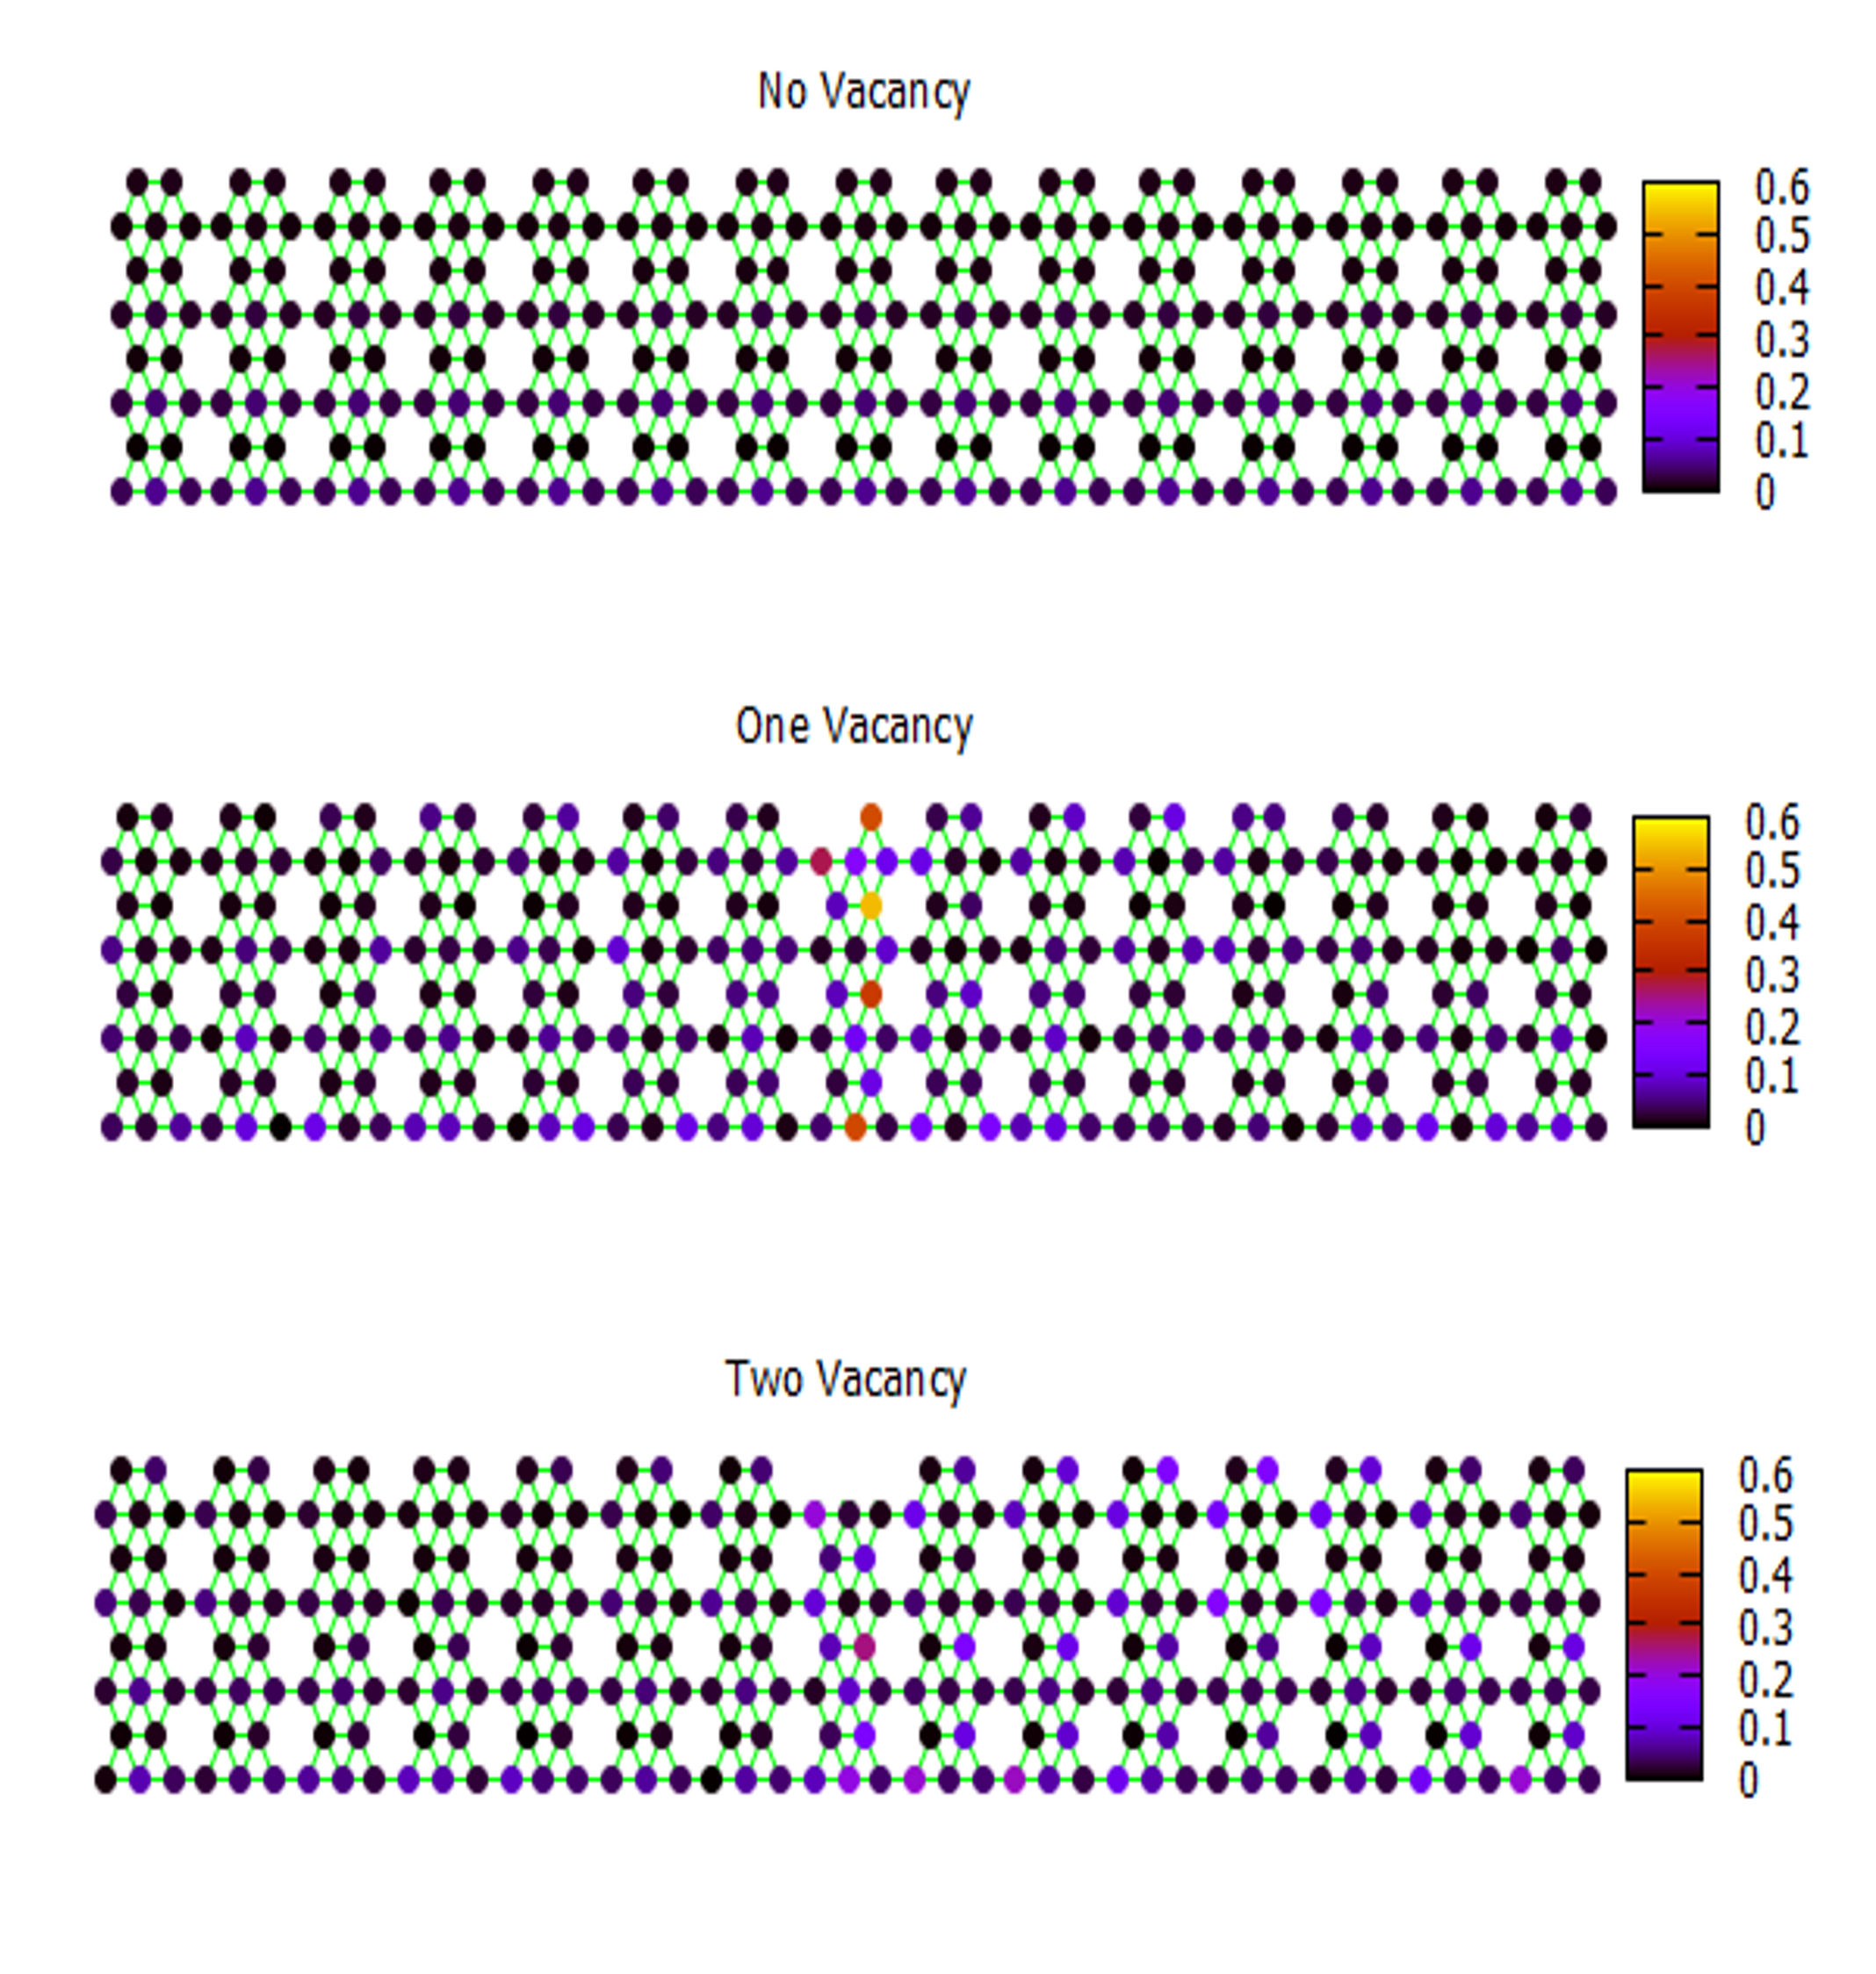
\includegraphics[width=1\linewidth]{./figures/Slide5.PNG}
\caption{در انرژی مربوط به اوج LDOS در نزدیکی انرژی فرمی، چگالی الکترونی فضایی حالات در کل محل نانوروبان بوروفن صندلی با یک محل خالی در لبه بالایی خالی، یک جای خالی، و دو جای خالی در وسط رسم شد. از نانو روبان}
\label{armVSLDOS}
\end{figure}
%%%% بنظر میرسد داشتن یک تصویر شماتیک برای این مبحث ضروری است که از مقاله واکی بایاشی بایدگرفت
در اینجا جهت تغییر ناپذیر انتقالی محور زیگزاگ را به عنوان محور x و محور y را عمود بر محور x در نظر می گیریم. این انتگرال عموماً یک عدد مختلط است، به این معنی که حالت کران طنین انداز می شود، یا به عبارت دیگر، یک حالت کران مجازی وجود دارد. برای نوارهای صندلی با عرض 18.59 \AA و با بی نظمی توزیع شده در هر دو لبه در طول 758.81 \AA با اختلال نسبتاً ضعیف $V_d = 1 eV$، BNR های صندلی صندلی از فلز به نیمه هادی تبدیل می شوند. با یک عمر محدود در حد پتانسیل نامتناهی V (یعنی یک جای خالی واحد در BNRها)، حالت کران مجازی به یک حالت کران کاملاً تعریف شده تبدیل می شود (با طول عمر نامحدود)، و سطح انرژی ناخالصی در $E = 0$ رخ می دهد. معادله شرودینگر می توان برای به دست آوردن حالت ویژه در فضای k با استفاده از این واقعیت که چگالی حالات برای یک سیستم دو بعدی با انرژی متناسب است استفاده کرد:
که در آن $G^0_A =\Sigma_k \phi_{Ak}$ با نرمال کردن توابع موج، متوجه می شویم که آنها دارای ویژگی غیرمحدود هستند، به عنوان مثال $\phi_{A}(r) = 0$ و $\phi_{B}(r) = 0$. بنابراین، هنگامی که یک جای خالی روی شبکه لانه زنبوری ایجاد می شود، سطح انرژی جای خالی در $E = 0$ با تابع موجی ظاهر می شود که دارای یک کاراکتر غیرمحدود است، یعنی دامنه آن در a(b) - سایت صفر است. همانطور که با معادله (16) مشاهده می شود، وجود جاهای خالی باعث سطح انرژی $E = 0$ می شود. از سوی دیگر، نشان داده شده است که حالت های لبه فقط در نانوروبان های زیگزاگ وجود دارد و نه در صندلی های صندلی. مشخص شده است که حالت های لبه را می توان به ترتیب در شکاف باند یا شکاف باند محلی در نیمه هادی ها و هادی ها نیز یافت [58]. علاوه بر این، در نانوروبانهای زیگزاگ، دو سطح انرژی در شکاف باند وجود دارد که میتوانند با هم جفت شوند و باعث فرورفتگی رسانایی شوند، در حالی که برای نانوروبانهای صندلی صندلی، هیچ کوپلینگی وجود ندارد. انرژی این افت های رسانایی مطابق با پیکربندی های ضد پیوند [60] است. بر اساس مدل فوق، اکنون ممکن است اثر یک نقص را بر رسانایی یک BNR به صورت کمی بررسی کنیم. محاسبات عددی ما LDOS تقریباً صفر را در محل پراکندگی نشان میدهد، که مربوط به کاراکتر نامحدود مدل مورد بررسی است. شکل 2.a رسانایی نانوروبان های زیگزاگی با عرض 18.59 \AA و طول 42.34 \AA (15 سوپرسل) را نشان می دهد، زمانی که یک ناخالصی با انواع قدرت های بالقوه در لبه بالایی سوپرسل واقع در وسط نانو نوار وجود دارد. در شکل 2.b، LDOS در نزدیکترین محل ناخالصی همسایه مانند بالا رسم شده است. همانطور که انتظار داریم، وجود ناخالصی باعث کاهش رسانایی می شود به طوری که در انرژی های خاص منجر به افت رسانایی می شود که به طور معادل با پیک در LDOS همراه است. همانطور که قبلا ذکر شد، یک شبکه لانه زنبوری پنهان در شبکه بوروفن $\beta_{12}$ وجود دارد، بنابراین افت رسانایی، همراه با قله های LDOS، می تواند به حالت های شبه موضعی که در مجاورت ناخالصی رخ می دهد نسبت داد
\subsection{چگالی حالتهای فضایی}
در این مقاله، رسانایی نانوروبانهای بورفن زیگزاگ و صندلی صندلی با نقصهای منفرد و اختلالات ضعیف در لبهها را در چارچوب مدل اتصال محکم با استفاده از تکنیک تابع گرین بررسی کردهایم. رسانایی نانوروبانهای بوروفن بکر رفتار گام به گام را نشان میدهد و تعداد کانالهای رسانایی در انرژی فرمی به عرض بوروفن بستگی دارد، به دلیل وجود اتم مرکزی در سلول واحد بوروفن، در تضاد واضح با مورد گرافن. ابتدا دو نوع نقص لبه را معرفی میکنیم، یعنی نقصهای منفرد شامل تک پراکندگی و تک خالی و اختلال ضعیف. نانوروبانهای بوروفن زیگزاگ همگی رفتار فلزی از خود نشان میدهند، در حالی که BNRهای صندلی راحتی بسته به عرض، رفتار فلزی یا نیمهرسانا را نشان میدهند. مشخص شده است که عیوب منفرد لبهای باعث حالتهای شبه موضعی میشوند و بنابراین افت رسانایی ظاهر میشوند. بنابراین، این نتایج ممکن است وجود شبکه لانه زنبوری پنهان را در داخل یک $\beta_{12}$-بوروفن با وجود ساختار شبکه مستطیلی آن تأیید کند. علاوه بر این، جای خالی یک اتمی و دو اتمی بر انتقال الکترون ها به طور قابل توجهی نسبت به مورد قبلی از طریق تشکیل حالت های شبه موضعی و افت رسانایی تأثیر می گذارد. در BNR های صندلی راحتی، جای خالی یک اتمی باعث شکسته شدن تقارن زیرشبکه می شود و بنابراین رسانایی را مهمتر از جای خالی دو اتمی تحت تاثیر قرار می دهد، در حالی که در BNR های زیگزاگ، جای خالی دو اتمی تقارن زیرشبکه را شکسته و انتقال را بیش از جای خالی یک اتمی تحت تاثیر قرار می دهد. توزیع تصادفی پراکندگی ضعیف روی لبههای BNR باعث میشود که محلیسازی اندرسون اتفاق بیفتد، که منجر به انتقال فلز به نیمهرسانا میشود. در BNR ها، طول محلی سازی اندرسون برای استحکام پتانسیل پایین بسیار طولانی است که با افزایش قدرت پتانسیل کاهش می یابد. با افزایش طول نانوروبان، رسانایی تا حد زیادی کاهش می یابد. در BNR های صندلی راحتی، پتانسیل های استحکام ضعیف باعث طول کوتاه تری نسبت به محلی سازی اندرسون در مقایسه با BNR های زیگزاگ می شود. علاوه بر این، طول محلی سازی به عرض BNR ها بستگی دارد به طوری که با افزایش عرض BNR ها، طول محلی سازی نیز افزایش می یابد.

\begin{figure}[!ht]
  \centering
  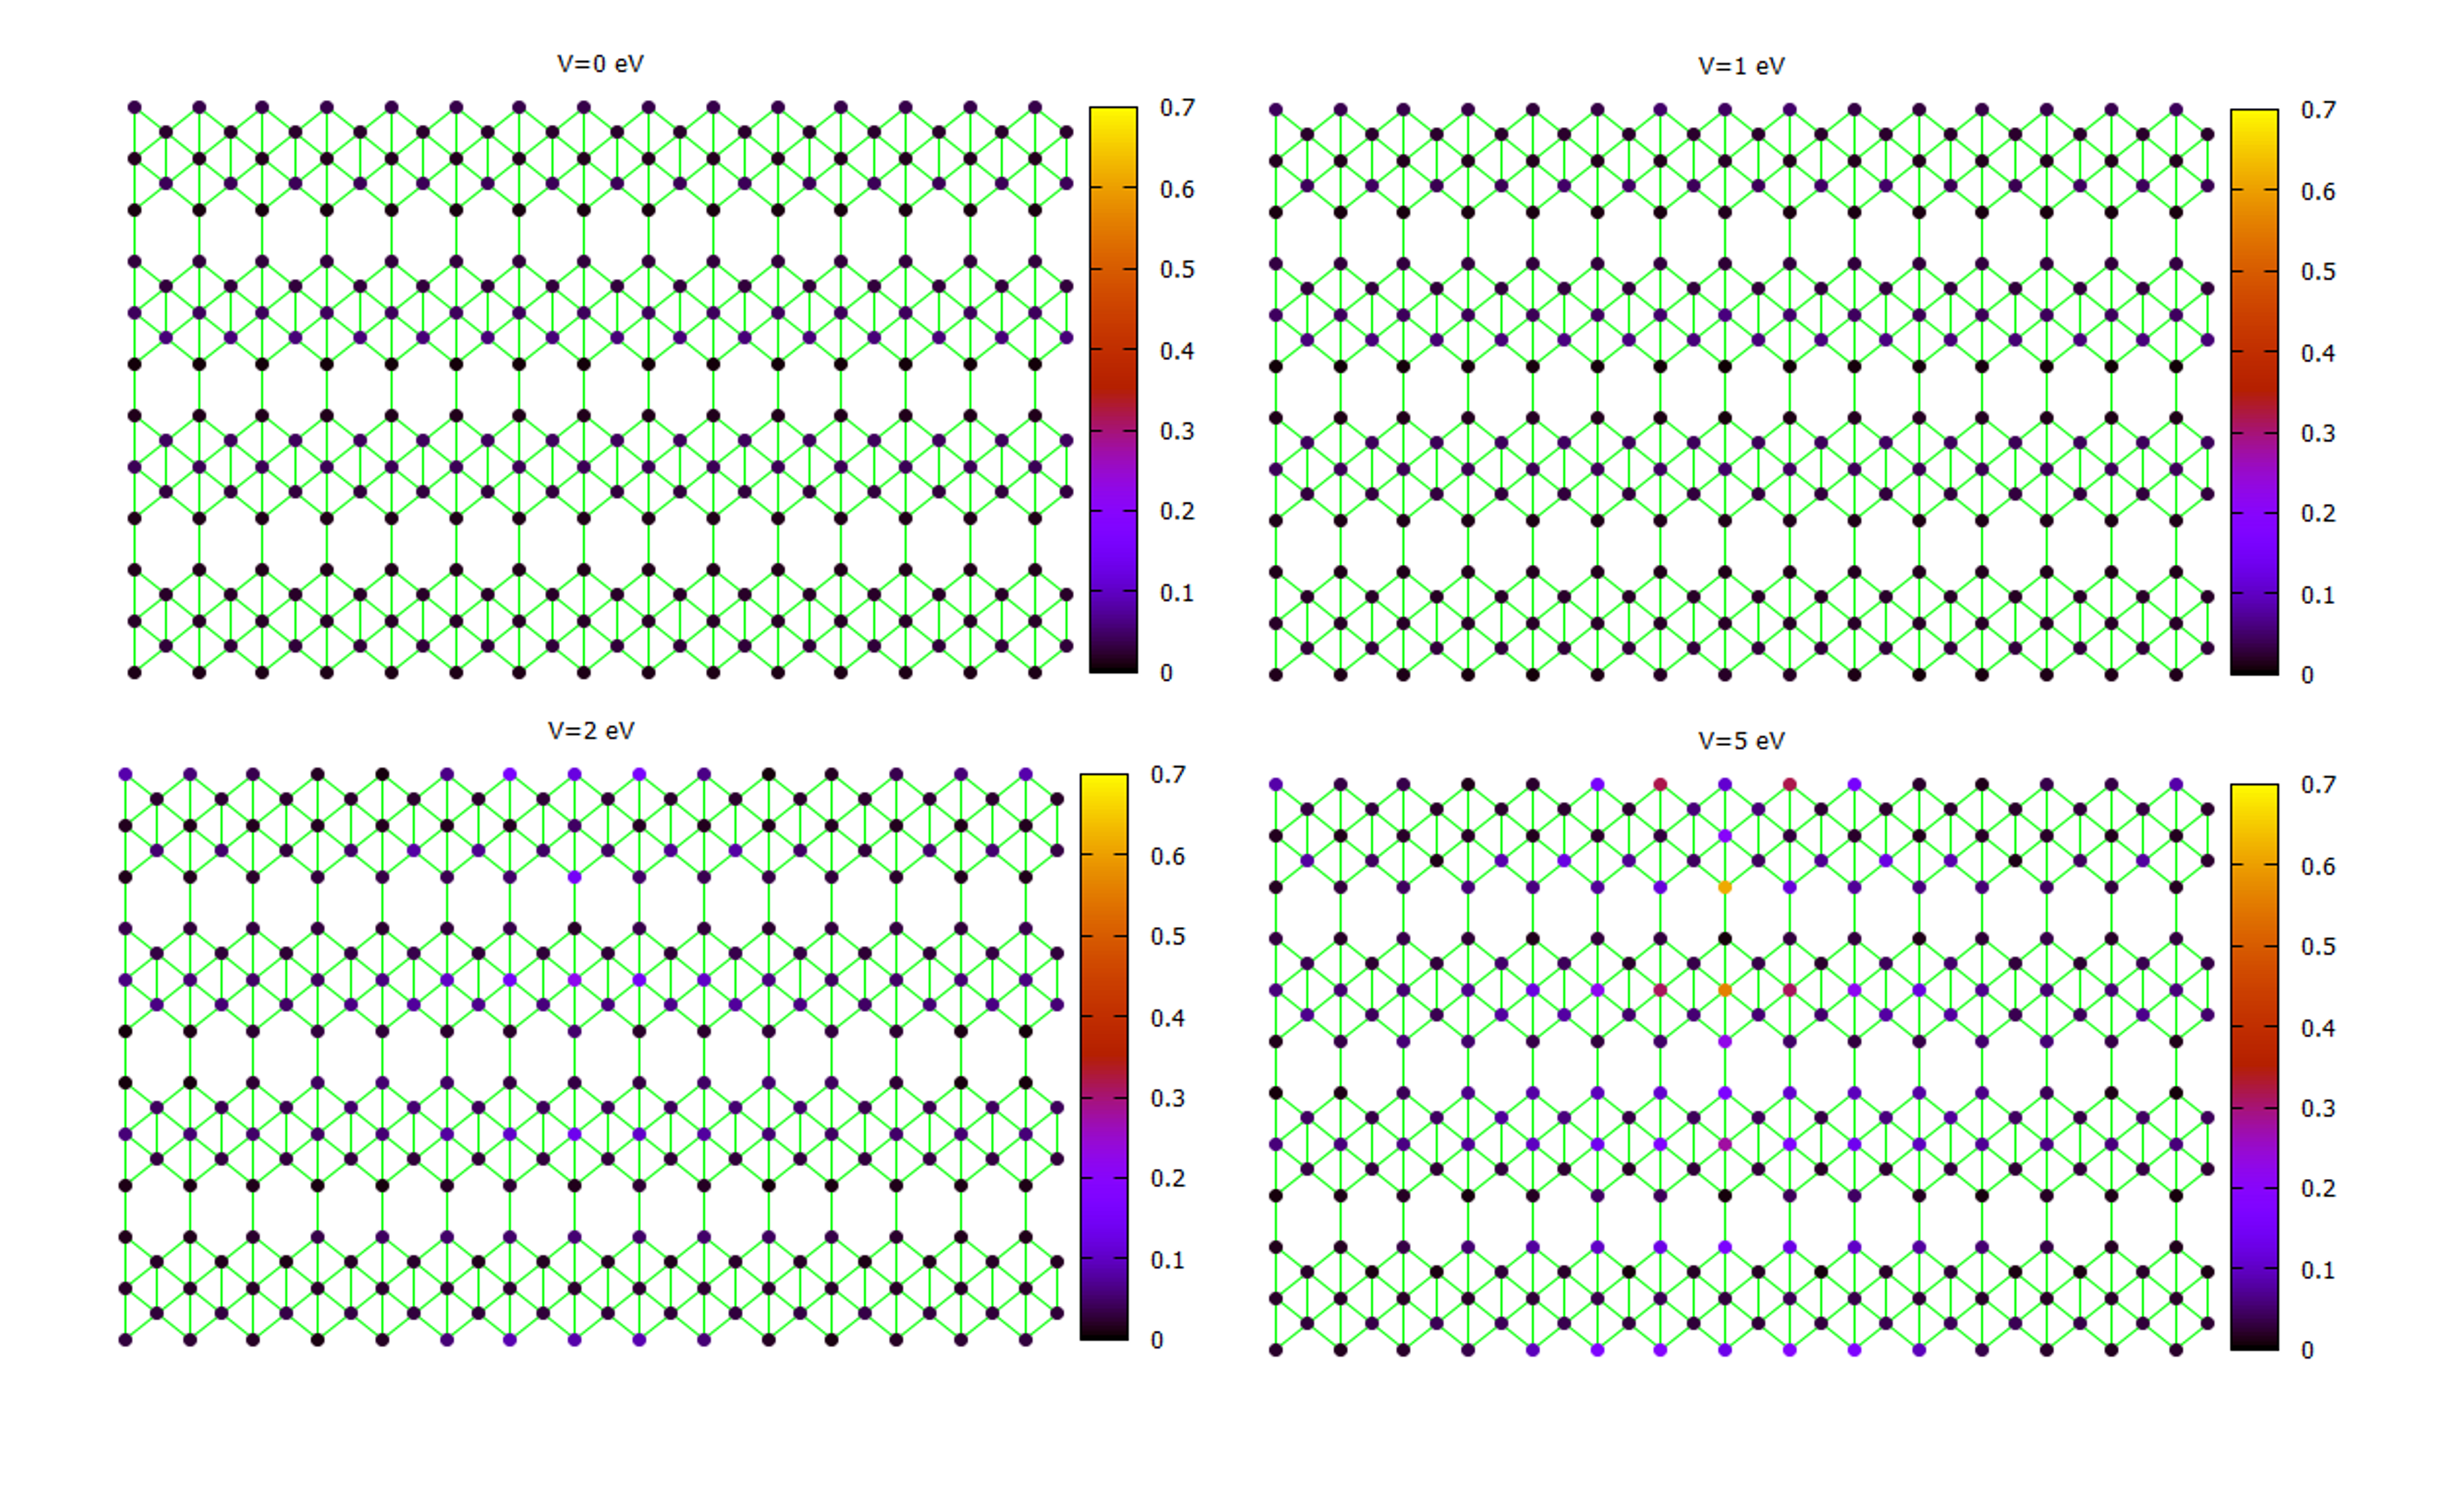
\includegraphics[width=1\linewidth]{./figures/Slide1.PNG}
  \caption{در انرژی مربوط به اوج LDOS نزدیک انرژی فرمی، چگالی الکترونی فضایی حالات در کل محل نانوروبان بوروفن زیگزاگ با یک محل پراکندگی در لبه بالایی با V=0،1،2،5 در وسط رسم شد. از نانو روبان}
  \label{zigCSLDOS}
\end{figure}

\begin{figure}[!ht]
  \centering
  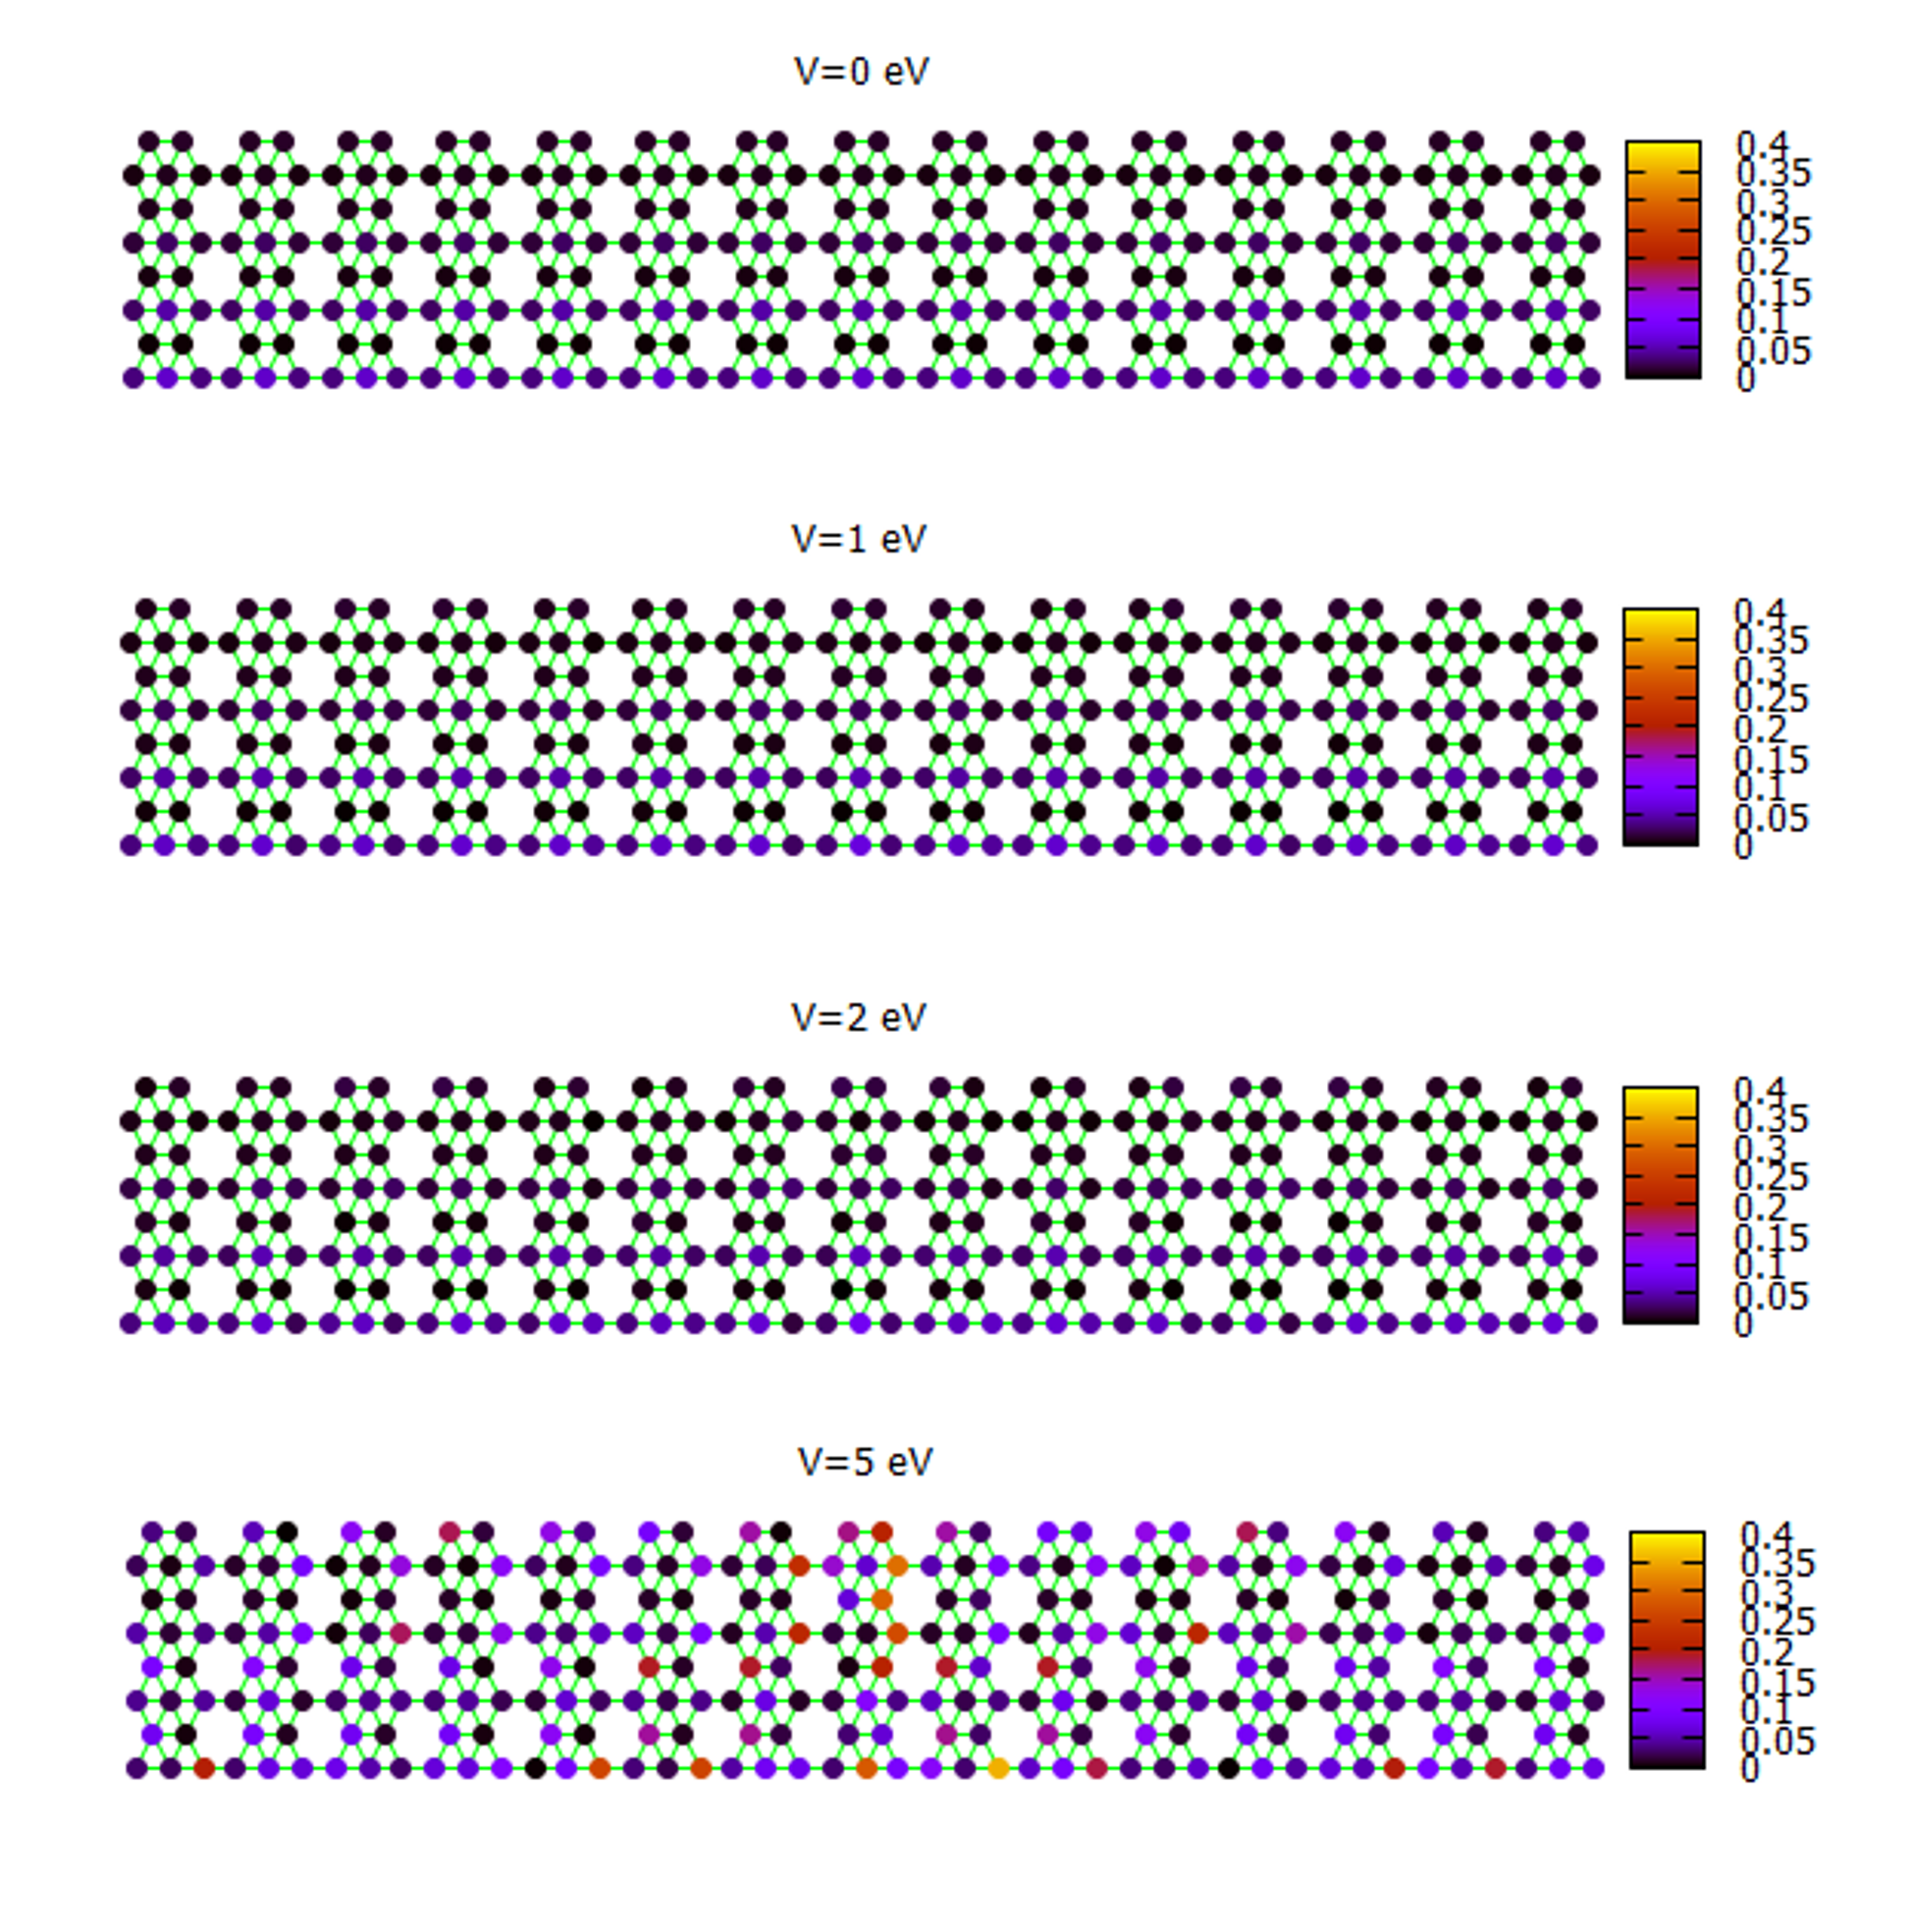
\includegraphics[width=1\linewidth]{./figures/Slide3.PNG}
  \caption{در انرژی مربوط به اوج LDOS نزدیک انرژی فرمی، چگالی الکترونی فضایی حالات در کل محل نانوروبان بوروفن صندلی با یک محل پراکندگی در لبه بالایی با V=0،1،2،5 در وسط رسم شد. از نانو روبان}
  \label{armCSLDOS}
\end{figure}
\begin{figure}[!ht]
    \centering
    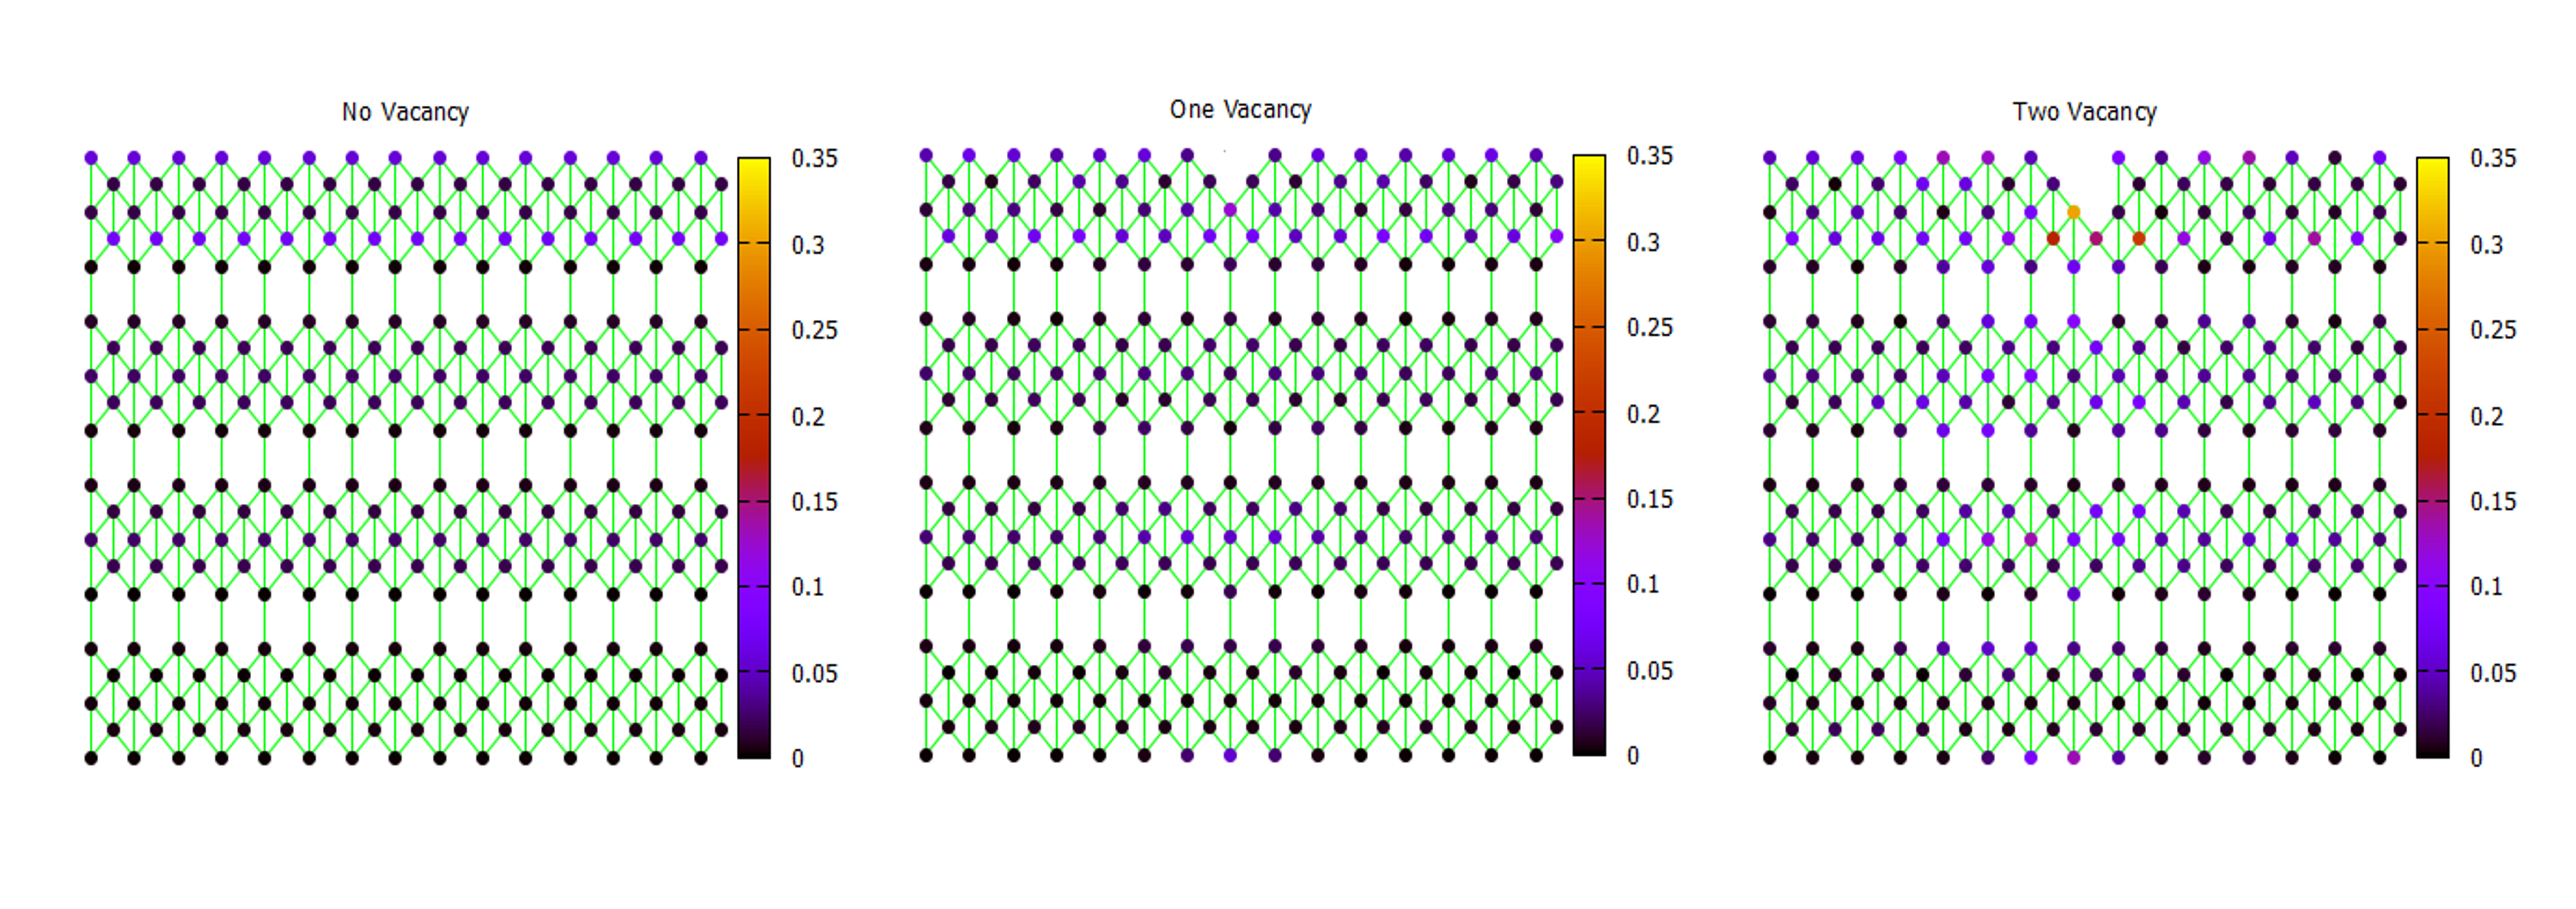
\includegraphics[width=1\linewidth]{./figures/Slide4.PNG}
    \caption{در انرژی مربوط به اوج LDOS در نزدیکی انرژی فرمی، چگالی الکترونی فضایی حالت‌ها در کل محل نانوروبان بوروفن زیگزاگ با یک محل خالی در لبه بالایی خالی، یک جای خالی و دو جای خالی در وسط رسم شد. از نانو روبان}
    \label{zigVSLDOS}
\end{figure}
\begin{figure}[!ht]
\centering
% GNUPLOT: LaTeX picture with Postscript
\begingroup
  % Encoding inside the plot.  In the header of your document, this encoding
  % should to defined, e.g., by using
  % \usepackage[cp1252,<other encodings>]{inputenc}
  % \inputencoding{cp1252}%
  \makeatletter
  \providecommand\color[2][]{%
    \GenericError{(gnuplot) \space\space\space\@spaces}{%
      Package color not loaded in conjunction with
      terminal option `colourtext'%
    }{See the gnuplot documentation for explanation.%
    }{Either use 'blacktext' in gnuplot or load the package
      color.sty in LaTeX.}%
    \renewcommand\color[2][]{}%
  }%
  \providecommand\includegraphics[2][]{%
    \GenericError{(gnuplot) \space\space\space\@spaces}{%
      Package graphicx or graphics not loaded%
    }{See the gnuplot documentation for explanation.%
    }{The gnuplot epslatex terminal needs graphicx.sty or graphics.sty.}%
    \renewcommand\includegraphics[2][]{}%
  }%
  \providecommand\rotatebox[2]{#2}%
  \@ifundefined{ifGPcolor}{%
    \newif\ifGPcolor
    \GPcolorfalse
  }{}%
  \@ifundefined{ifGPblacktext}{%
    \newif\ifGPblacktext
    \GPblacktexttrue
  }{}%
  % define a \g@addto@macro without @ in the name:
  \let\gplgaddtomacro\g@addto@macro
  % define empty templates for all commands taking text:
  \gdef\gplbacktext{}%
  \gdef\gplfronttext{}%
  \makeatother
  \ifGPblacktext
    % no textcolor at all
    \def\colorrgb#1{}%
    \def\colorgray#1{}%
  \else
    % gray or color?
    \ifGPcolor
      \def\colorrgb#1{\color[rgb]{#1}}%
      \def\colorgray#1{\color[gray]{#1}}%
      \expandafter\def\csname LTw\endcsname{\color{white}}%
      \expandafter\def\csname LTb\endcsname{\color{black}}%
      \expandafter\def\csname LTa\endcsname{\color{black}}%
      \expandafter\def\csname LT0\endcsname{\color[rgb]{1,0,0}}%
      \expandafter\def\csname LT1\endcsname{\color[rgb]{0,1,0}}%
      \expandafter\def\csname LT2\endcsname{\color[rgb]{0,0,1}}%
      \expandafter\def\csname LT3\endcsname{\color[rgb]{1,0,1}}%
      \expandafter\def\csname LT4\endcsname{\color[rgb]{0,1,1}}%
      \expandafter\def\csname LT5\endcsname{\color[rgb]{1,1,0}}%
      \expandafter\def\csname LT6\endcsname{\color[rgb]{0,0,0}}%
      \expandafter\def\csname LT7\endcsname{\color[rgb]{1,0.3,0}}%
      \expandafter\def\csname LT8\endcsname{\color[rgb]{0.5,0.5,0.5}}%
    \else
      % gray
      \def\colorrgb#1{\color{black}}%
      \def\colorgray#1{\color[gray]{#1}}%
      \expandafter\def\csname LTw\endcsname{\color{white}}%
      \expandafter\def\csname LTb\endcsname{\color{black}}%
      \expandafter\def\csname LTa\endcsname{\color{black}}%
      \expandafter\def\csname LT0\endcsname{\color{black}}%
      \expandafter\def\csname LT1\endcsname{\color{black}}%
      \expandafter\def\csname LT2\endcsname{\color{black}}%
      \expandafter\def\csname LT3\endcsname{\color{black}}%
      \expandafter\def\csname LT4\endcsname{\color{black}}%
      \expandafter\def\csname LT5\endcsname{\color{black}}%
      \expandafter\def\csname LT6\endcsname{\color{black}}%
      \expandafter\def\csname LT7\endcsname{\color{black}}%
      \expandafter\def\csname LT8\endcsname{\color{black}}%
    \fi
  \fi
    \setlength{\unitlength}{0.0500bp}%
    \ifx\gptboxheight\undefined%
      \newlength{\gptboxheight}%
      \newlength{\gptboxwidth}%
      \newsavebox{\gptboxtext}%
    \fi%
    \setlength{\fboxrule}{0.5pt}%
    \setlength{\fboxsep}{1pt}%
\begin{picture}(5040.00,4320.00)%
    \gplgaddtomacro\gplbacktext{%
      \csname LTb\endcsname%%
      \put(550,704){\makebox(0,0)[r]{\strut{}$0$}}%
      \put(550,1128){\makebox(0,0)[r]{\strut{}$1$}}%
      \put(550,1553){\makebox(0,0)[r]{\strut{}$2$}}%
      \put(550,1977){\makebox(0,0)[r]{\strut{}$3$}}%
      \put(550,2402){\makebox(0,0)[r]{\strut{}$4$}}%
      \put(550,2826){\makebox(0,0)[r]{\strut{}$5$}}%
      \put(550,3250){\makebox(0,0)[r]{\strut{}$6$}}%
      \put(550,3675){\makebox(0,0)[r]{\strut{}$7$}}%
      \put(550,4099){\makebox(0,0)[r]{\strut{}$8$}}%
      \put(682,484){\makebox(0,0){\strut{}$-2$}}%
      \put(1177,484){\makebox(0,0){\strut{}$-1.5$}}%
      \put(1672,484){\makebox(0,0){\strut{}$-1$}}%
      \put(2167,484){\makebox(0,0){\strut{}$-0.5$}}%
      \put(2663,484){\makebox(0,0){\strut{}$0$}}%
      \put(3158,484){\makebox(0,0){\strut{}$0.5$}}%
      \put(3653,484){\makebox(0,0){\strut{}$1$}}%
      \put(4148,484){\makebox(0,0){\strut{}$1.5$}}%
      \put(4643,484){\makebox(0,0){\strut{}$2$}}%
    }%
    \gplgaddtomacro\gplfronttext{%
      \csname LTb\endcsname%%
      \put(198,2401){\rotatebox{-270}{\makebox(0,0){\strut{}$G/G_0$}}}%
      \put(2662,154){\makebox(0,0){\strut{}Energy(eV)}}%
      \csname LTb\endcsname%%
      \put(3656,3926){\makebox(0,0)[r]{\strut{}pristine ZBNR}}%
      \csname LTb\endcsname%%
      \put(3656,3706){\makebox(0,0)[r]{\strut{}V=0.25 eV}}%
      \csname LTb\endcsname%%
      \put(3656,3486){\makebox(0,0)[r]{\strut{}V=0.5 eV}}%
      \csname LTb\endcsname%%
      \put(3656,3266){\makebox(0,0)[r]{\strut{}V=2 eV}}%
    }%
    \gplbacktext
    \put(0,0){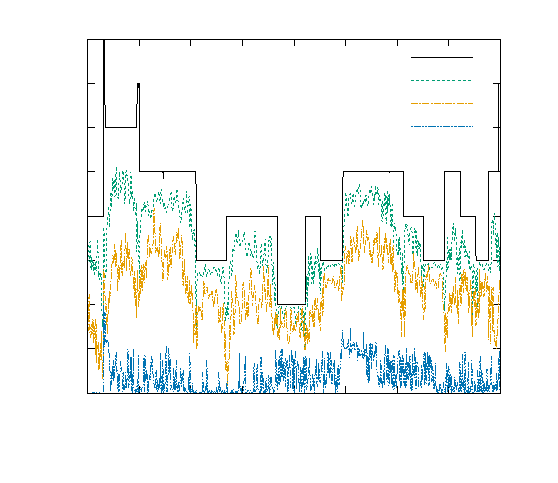
\includegraphics[width={253.00bp},height={217.00bp}]{zigzagdisorder}}%
    \gplfronttext
  \end{picture}%
\endgroup

\caption{رسانایی در مقابل انرژی برای نوارهای زیگزاگی با عرض $10.24$\AA و با بی نظمی در هر دو لبه به طول $876.68 $\AA توزیع شده است
با یک اختلال نسبتا ضعیف $V_d=2\;eV$، BNR های زیگزاگی از فلز به نیمه هادی تبدیل می شوند.}
\label{zigzagdisorder}
\end{figure}

توزیع چگالی حالت ها در همه مکان های نانوروبان به انرژی بستگی دارد. توزیع چگالی حالت ها حول E=-0.034 ترسیم شده است در شکل 3. شکل 3 نشان می دهد که در حالی که هیچ پراکنده ای روی نانوروبان وجود ندارد، توزیع چگالی حالت ها تقریباً در همه مکان ها برابر است. با قرار دادن پراکنده در لبه بالایی سوپرسل میانی نانوروبان معادل شکل 1، توزیع چگالی حالت ها در اطراف ابرسلول میانی افزایش می یابد. با افزایش قدرت پراکندگی، چگالی حالات در اطراف ابرسلول مرکزی افزایش می یابد. با افزایش قدرت پراکنده، توزیع چگالی حالت ها به سمت نزدیکترین محل به پراکنده مشهود است. در شکل 4.a و شکل 4.b، رسانایی و LDOS به ترتیب برای ABNR ها با عرض 10.24 \AA رسم شده است. ناخالصی در لبه بالایی سوپرسل میانی نانوروبان قرار دارد. در هر دو BNR صندلی راحتی و زیگزاگ، ناخالصی های ضعیف نمی توانند بر رسانایی تأثیر بگذارند. با این حال، با افزایش قدرت پتانسیل ناخالصی ها، شیب رسانایی در اطراف انرژی فرمی همزمان با پیک LDOS در محل مجاور ناخالصی ایجاد می شود. بنابراین حالت های شبه موضعی را می توان در ناخالصی های قوی مشاهده کرد. در ZBNR ها، فرورفتگی های رسانایی، در نتیجه ناخالصی لبه، به وضوح در لبه نوار مشاهده می شود، و عرض شیب ها زمانی که قدرت پتانسیل نقص مشاهده می شود، قابل توجه می شود. بیشتر از $2 eV$ با این حال، در ABNR ها، یک شیب رسانایی در اطراف انرژی فرمی ظاهر می شود، جایی که یک پیک معادل، مرتبط با حالت های شبه موضعی را می توان در LDOS مشاهده کرد، زمانی که نقص قدرت بالقوه $5 eV$ باشد. شکل 5 افزایش چگالی حالت ها را در اطراف سوپرسل میانی نانوروبان با لبه های صندلی با انرژی 0.19 نشان می دهد. علاوه بر این، نشان می دهد که یک پراکنده روی لبه بوروفن با لبه صندلی دارای تأثیر بیشتری نسبت به یک پراکنده روی لبه بوروفن با لبه زیگزاگ است. بنابراین این موضوع مقایسه رسانایی و LDOS در شکل 2 و 4 را تایید می کند که اثر پراکندگی بر روی رسانایی و نمودار LDOS بوروفن با لبه صندلی صندلی قابل توجه تر است. در شکل 8، رسانایی و LDOS مربوطه برای ABNR ها با عرض 10.24 \AA (4 سلول واحد در سوپرسل) در دو حالت خالی، یک یا دو اتم خالی ترسیم شده است. تأثیر جای خالی لبه تک اتمی و جای خالی لبه دو اتمی بر رسانایی ABNR ها کاملاً متفاوت است. در حالت اول، فرورفتگیهای رسانایی در لبههای نوارها ظاهر میشوند، که متفاوت از تکینگیهای Van-Hoff سیستم بکر است، بنابراین شواهدی مبنی بر وجود شبه ذرات در آن انرژی وجود دارد. قبلاً دیده شده است که یک شبکه لانه زنبوری پنهان در ساختار شبکه $\beta_{12}$ وجود دارد و متعاقباً مشابه گرافن، ممکن است دو زیرشبکه تعریف شود. در نتیجه، شیب رسانایی برجسته در دومی، که با یک قله بزرگ در LDOS در انرژی فرمی همراه است، از شکستن تقارن زیرشبکه نشات میگیرد. همانطور که قبلا ذکر کردیم، در حالی که قدرت پراکندگی را تا بی نهایت افزایش می دهیم، به نانوروبان با یک جای خالی در لبه می رسیم. بنابراین، چگالی حالتها در اطراف سوپرسل میانی دارای بیشترین غلظت و تقریباً مقدار قابل توجهی LDOS است که در نزدیکترین مکان به جای خالی قرار میگیرد. شکست تقارن انتقالی در حضور یک جای خالی در نانوروبان با لبه صندلی در شکل 9 مشاهده شده است و نتایج قبلی ذکر شده در شکل 8 را تایید می کند. ZBNRهای با جای خالی لبهای رفتاری مشابه با جای خالی لبههای نانوروبانهای گرافن صندلی راحتی دارند، زیرا فرورفتگیهای رسانایی در لبههای نوارهای مربوط به قلههای LDOS رخ میدهد تا حالتهای شبه موضعی ممکن است نتیجهگیری شود. با این حال، در مورد جاهای خالی لبه دو اتمی در ZBNR، یک شیب رسانایی بزرگ با یک LDOS بزرگ معادل در انرژی فرمی دیده میشود، مانند مورد ABNR، که کاملاً با GNRs متناقض است.

این را می توان با شکستن تقارن توضیح داد. زیرشبکه به دلیل وجود اتم میانی در سلول واحد در لبه. همچنین، در بوروفن با لبه زیگزاگ (شکل 7)، مانند ABNRها، حد نهایی LDOS در نزدیکترین محل پراکنده نشان داده شده است و می توان مشاهده کرد که نتایج قبلی به دست آمده از شکل 6 را تایید می کند.

\subsection{پراکندگی اندرسون}
 در اینجا باید به کلیت پراکندگی اندرسون بپردازیم. و شقوق مختلف آنرا بیان کینم و در اخر نتایج خود رادر مورد بورفین اعلام کنیم.
% a† i (ai ) عملگرهای ایجاد الکترون (نابودی) در الکترون π در جایگاه i هستند، εi انرژی در محل در i-site و tij انرژی پرش نزدیکترین همسایه است. سرعت فرمی در جهات مختلف با انبساط همیلتونی در فضای فوریه حول یک نقطه شبکه متقابل به دست می آید، به طوری که انرژی های جهشی مختلف در بوروفن منجر به سرعت های متفاوتی در آن می شود. شایان ذکر است که به منظور شبیه سازی وجود ناخالصی ها، اصطلاحاً پراکندگی ضعیف، عبارت دیگری حاوی انرژی در محل ωi به هامیلتونین اضافه می شود. از آنجایی که مدل وارونگی غیر متقارن با آزمایشات [26] سازگار است، ما از ضرایب مربوطه در هامیلتونی استفاده می کنیم. یک لایه $\beta_{12}$ را به سه قسمت تقسیم می کنیم. نانوروبان، به عنوان بخش مرکزی سیستم، ناحیه پراکنده ای است که توسط دو سرب نیمه نامتناهی احاطه شده است. ما نانوروبان را به عنوان یک سیم 1 بعدی با دو نوع لبه در نظر می گیریم. بسته به محل سرنخ ها، با سیم 1 بعدی ایجاد شده از نانوروبان های بوروفن زیگزاگ (ZBNRs) یا نانوروبان های بوروفن \lr{Armchair (ABNRs)} مواجه می شویم. به منظور بررسی رسانایی $\beta_{12}$، از روش لوپز سانچو برای محاسبه تابع گرین سطح [56] به صورت زیر استفاده می شود:
% که در آن Hl,l همیلتونین ابرسلولهای BNRها است و Hl,l+1 ماتریس برهمکنش بین BNRهای مجاور است. ، ̃ ماتریس های انتقالی هستند که توسط عناصر ماتریس همیلتونی با اتصال محکم با استفاده از روش بازگشتی به دست می آیند [48].

\begin{figure}[!ht]
    \centering
      % GNUPLOT: LaTeX picture with Postscript
\begingroup
  % Encoding inside the plot.  In the header of your document, this encoding
  % should to defined, e.g., by using
  % \usepackage[cp1252,<other encodings>]{inputenc}
  % \inputencoding{cp1252}%
  \makeatletter
  \providecommand\color[2][]{%
    \GenericError{(gnuplot) \space\space\space\@spaces}{%
      Package color not loaded in conjunction with
      terminal option `colourtext'%
    }{See the gnuplot documentation for explanation.%
    }{Either use 'blacktext' in gnuplot or load the package
      color.sty in LaTeX.}%
    \renewcommand\color[2][]{}%
  }%
  \providecommand\includegraphics[2][]{%
    \GenericError{(gnuplot) \space\space\space\@spaces}{%
      Package graphicx or graphics not loaded%
    }{See the gnuplot documentation for explanation.%
    }{The gnuplot epslatex terminal needs graphicx.sty or graphics.sty.}%
    \renewcommand\includegraphics[2][]{}%
  }%
  \providecommand\rotatebox[2]{#2}%
  \@ifundefined{ifGPcolor}{%
    \newif\ifGPcolor
    \GPcolorfalse
  }{}%
  \@ifundefined{ifGPblacktext}{%
    \newif\ifGPblacktext
    \GPblacktexttrue
  }{}%
  % define a \g@addto@macro without @ in the name:
  \let\gplgaddtomacro\g@addto@macro
  % define empty templates for all commands taking text:
  \gdef\gplbacktext{}%
  \gdef\gplfronttext{}%
  \makeatother
  \ifGPblacktext
    % no textcolor at all
    \def\colorrgb#1{}%
    \def\colorgray#1{}%
  \else
    % gray or color?
    \ifGPcolor
      \def\colorrgb#1{\color[rgb]{#1}}%
      \def\colorgray#1{\color[gray]{#1}}%
      \expandafter\def\csname LTw\endcsname{\color{white}}%
      \expandafter\def\csname LTb\endcsname{\color{black}}%
      \expandafter\def\csname LTa\endcsname{\color{black}}%
      \expandafter\def\csname LT0\endcsname{\color[rgb]{1,0,0}}%
      \expandafter\def\csname LT1\endcsname{\color[rgb]{0,1,0}}%
      \expandafter\def\csname LT2\endcsname{\color[rgb]{0,0,1}}%
      \expandafter\def\csname LT3\endcsname{\color[rgb]{1,0,1}}%
      \expandafter\def\csname LT4\endcsname{\color[rgb]{0,1,1}}%
      \expandafter\def\csname LT5\endcsname{\color[rgb]{1,1,0}}%
      \expandafter\def\csname LT6\endcsname{\color[rgb]{0,0,0}}%
      \expandafter\def\csname LT7\endcsname{\color[rgb]{1,0.3,0}}%
      \expandafter\def\csname LT8\endcsname{\color[rgb]{0.5,0.5,0.5}}%
    \else
      % gray
      \def\colorrgb#1{\color{black}}%
      \def\colorgray#1{\color[gray]{#1}}%
      \expandafter\def\csname LTw\endcsname{\color{white}}%
      \expandafter\def\csname LTb\endcsname{\color{black}}%
      \expandafter\def\csname LTa\endcsname{\color{black}}%
      \expandafter\def\csname LT0\endcsname{\color{black}}%
      \expandafter\def\csname LT1\endcsname{\color{black}}%
      \expandafter\def\csname LT2\endcsname{\color{black}}%
      \expandafter\def\csname LT3\endcsname{\color{black}}%
      \expandafter\def\csname LT4\endcsname{\color{black}}%
      \expandafter\def\csname LT5\endcsname{\color{black}}%
      \expandafter\def\csname LT6\endcsname{\color{black}}%
      \expandafter\def\csname LT7\endcsname{\color{black}}%
      \expandafter\def\csname LT8\endcsname{\color{black}}%
    \fi
  \fi
    \setlength{\unitlength}{0.0500bp}%
    \ifx\gptboxheight\undefined%
      \newlength{\gptboxheight}%
      \newlength{\gptboxwidth}%
      \newsavebox{\gptboxtext}%
    \fi%
    \setlength{\fboxrule}{0.5pt}%
    \setlength{\fboxsep}{1pt}%
\begin{picture}(5040.00,4320.00)%
    \gplgaddtomacro\gplbacktext{%
      \csname LTb\endcsname%%
      \put(550,704){\makebox(0,0)[r]{\strut{}$0$}}%
      \put(550,1270){\makebox(0,0)[r]{\strut{}$1$}}%
      \put(550,1836){\makebox(0,0)[r]{\strut{}$2$}}%
      \put(550,2402){\makebox(0,0)[r]{\strut{}$3$}}%
      \put(550,2967){\makebox(0,0)[r]{\strut{}$4$}}%
      \put(550,3533){\makebox(0,0)[r]{\strut{}$5$}}%
      \put(550,4099){\makebox(0,0)[r]{\strut{}$6$}}%
      \put(682,484){\makebox(0,0){\strut{}$-2$}}%
      \put(1342,484){\makebox(0,0){\strut{}$-1.5$}}%
      \put(2002,484){\makebox(0,0){\strut{}$-1$}}%
      \put(2662,484){\makebox(0,0){\strut{}$-0.5$}}%
      \put(3323,484){\makebox(0,0){\strut{}$0$}}%
      \put(3983,484){\makebox(0,0){\strut{}$0.5$}}%
      \put(4643,484){\makebox(0,0){\strut{}$1$}}%
    }%
    \gplgaddtomacro\gplfronttext{%
      \csname LTb\endcsname%%
      \put(198,2401){\rotatebox{-270}{\makebox(0,0){\strut{}$G/G_0$}}}%
      \put(2662,154){\makebox(0,0){\strut{}Energy(eV)}}%
      \csname LTb\endcsname%%
      \put(3656,3926){\makebox(0,0)[r]{\strut{}pristine ABNR}}%
      \csname LTb\endcsname%%
      \put(3656,3706){\makebox(0,0)[r]{\strut{}V=0.25 eV}}%
      \csname LTb\endcsname%%
      \put(3656,3486){\makebox(0,0)[r]{\strut{}V=0.5 eV}}%
      \csname LTb\endcsname%%
      \put(3656,3266){\makebox(0,0)[r]{\strut{}V=1 eV}}%
    }%
    \gplbacktext
    \put(0,0){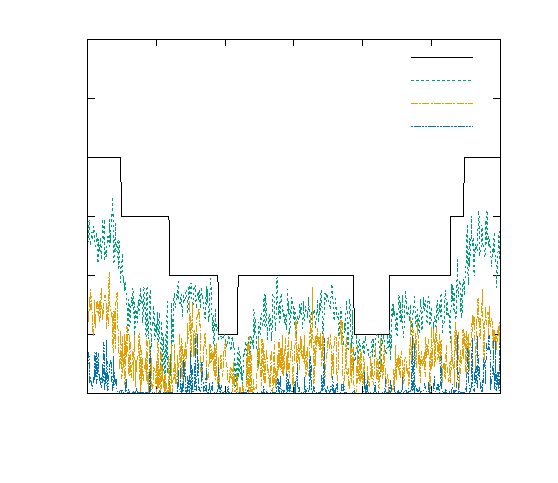
\includegraphics[width={253.00bp},height={217.00bp}]{armdisorder}}%
    \gplfronttext
  \end{picture}%
\endgroup

      \caption{رسانایی در مقابل انرژی برای نوارهای صندلی با عرض $18.59$\AA و با بی نظمی توزیع شده در هر دو لبه در طول $758.81$\AA با اختلال نسبتا ضعیف $V_d=1\;eV$، BNRهای صندلی از فلز به نیمه هادی تبدیل می شوند.}
      \label{armdisorder}
    \end{figure}
    
    \begin{figure*}[!ht]
      \centering
      % GNUPLOT: LaTeX picture with Postscript
\begingroup
  % Encoding inside the plot.  In the header of your document, this encoding
  % should to defined, e.g., by using
  % \usepackage[cp1252,<other encodings>]{inputenc}
  % \inputencoding{cp1252}%
  \makeatletter
  \providecommand\color[2][]{%
    \GenericError{(gnuplot) \space\space\space\@spaces}{%
      Package color not loaded in conjunction with
      terminal option `colourtext'%
    }{See the gnuplot documentation for explanation.%
    }{Either use 'blacktext' in gnuplot or load the package
      color.sty in LaTeX.}%
    \renewcommand\color[2][]{}%
  }%
  \providecommand\includegraphics[2][]{%
    \GenericError{(gnuplot) \space\space\space\@spaces}{%
      Package graphicx or graphics not loaded%
    }{See the gnuplot documentation for explanation.%
    }{The gnuplot epslatex terminal needs graphicx.sty or graphics.sty.}%
    \renewcommand\includegraphics[2][]{}%
  }%
  \providecommand\rotatebox[2]{#2}%
  \@ifundefined{ifGPcolor}{%
    \newif\ifGPcolor
    \GPcolorfalse
  }{}%
  \@ifundefined{ifGPblacktext}{%
    \newif\ifGPblacktext
    \GPblacktexttrue
  }{}%
  % define a \g@addto@macro without @ in the name:
  \let\gplgaddtomacro\g@addto@macro
  % define empty templates for all commands taking text:
  \gdef\gplbacktext{}%
  \gdef\gplfronttext{}%
  \makeatother
  \ifGPblacktext
    % no textcolor at all
    \def\colorrgb#1{}%
    \def\colorgray#1{}%
  \else
    % gray or color?
    \ifGPcolor
      \def\colorrgb#1{\color[rgb]{#1}}%
      \def\colorgray#1{\color[gray]{#1}}%
      \expandafter\def\csname LTw\endcsname{\color{white}}%
      \expandafter\def\csname LTb\endcsname{\color{black}}%
      \expandafter\def\csname LTa\endcsname{\color{black}}%
      \expandafter\def\csname LT0\endcsname{\color[rgb]{1,0,0}}%
      \expandafter\def\csname LT1\endcsname{\color[rgb]{0,1,0}}%
      \expandafter\def\csname LT2\endcsname{\color[rgb]{0,0,1}}%
      \expandafter\def\csname LT3\endcsname{\color[rgb]{1,0,1}}%
      \expandafter\def\csname LT4\endcsname{\color[rgb]{0,1,1}}%
      \expandafter\def\csname LT5\endcsname{\color[rgb]{1,1,0}}%
      \expandafter\def\csname LT6\endcsname{\color[rgb]{0,0,0}}%
      \expandafter\def\csname LT7\endcsname{\color[rgb]{1,0.3,0}}%
      \expandafter\def\csname LT8\endcsname{\color[rgb]{0.5,0.5,0.5}}%
    \else
      % gray
      \def\colorrgb#1{\color{black}}%
      \def\colorgray#1{\color[gray]{#1}}%
      \expandafter\def\csname LTw\endcsname{\color{white}}%
      \expandafter\def\csname LTb\endcsname{\color{black}}%
      \expandafter\def\csname LTa\endcsname{\color{black}}%
      \expandafter\def\csname LT0\endcsname{\color{black}}%
      \expandafter\def\csname LT1\endcsname{\color{black}}%
      \expandafter\def\csname LT2\endcsname{\color{black}}%
      \expandafter\def\csname LT3\endcsname{\color{black}}%
      \expandafter\def\csname LT4\endcsname{\color{black}}%
      \expandafter\def\csname LT5\endcsname{\color{black}}%
      \expandafter\def\csname LT6\endcsname{\color{black}}%
      \expandafter\def\csname LT7\endcsname{\color{black}}%
      \expandafter\def\csname LT8\endcsname{\color{black}}%
    \fi
  \fi
    \setlength{\unitlength}{0.0500bp}%
    \ifx\gptboxheight\undefined%
      \newlength{\gptboxheight}%
      \newlength{\gptboxwidth}%
      \newsavebox{\gptboxtext}%
    \fi%
    \setlength{\fboxrule}{0.5pt}%
    \setlength{\fboxsep}{1pt}%
\begin{picture}(7200.00,5040.00)%
    \gplgaddtomacro\gplbacktext{%
      \csname LTb\endcsname%%
      \put(814,704){\makebox(0,0)[r]{\strut{}$0$}}%
      \put(814,1161){\makebox(0,0)[r]{\strut{}$0.5$}}%
      \put(814,1618){\makebox(0,0)[r]{\strut{}$1$}}%
      \put(814,2076){\makebox(0,0)[r]{\strut{}$1.5$}}%
      \put(814,2533){\makebox(0,0)[r]{\strut{}$2$}}%
      \put(814,2990){\makebox(0,0)[r]{\strut{}$2.5$}}%
      \put(814,3447){\makebox(0,0)[r]{\strut{}$3$}}%
      \put(814,3905){\makebox(0,0)[r]{\strut{}$3.5$}}%
      \put(814,4362){\makebox(0,0)[r]{\strut{}$4$}}%
      \put(814,4819){\makebox(0,0)[r]{\strut{}$4.5$}}%
      \put(946,484){\makebox(0,0){\strut{}$0$}}%
      \put(1197,484){\makebox(0,0){\strut{}$2$}}%
      \put(1448,484){\makebox(0,0){\strut{}$4$}}%
      \put(1698,484){\makebox(0,0){\strut{}$6$}}%
      \put(1949,484){\makebox(0,0){\strut{}$8$}}%
      \put(2200,484){\makebox(0,0){\strut{}$10$}}%
      \put(2451,484){\makebox(0,0){\strut{}$12$}}%
      \put(2701,484){\makebox(0,0){\strut{}$14$}}%
      \put(2952,484){\makebox(0,0){\strut{}$16$}}%
      \put(3203,484){\makebox(0,0){\strut{}$18$}}%
      \put(1172,4613){\makebox(0,0)[l]{\strut{}(a)}}%
    }%
    \gplgaddtomacro\gplfronttext{%
      \csname LTb\endcsname%%
      \put(198,2761){\rotatebox{-270}{\makebox(0,0){\strut{}$G/G_0$}}}%
      \put(2074,154){\makebox(0,0){\strut{}Length(nm)$*10^{1}$}}%
      \csname LTb\endcsname%%
      \put(2216,4646){\makebox(0,0)[r]{\strut{}W=4}}%
      \csname LTb\endcsname%%
      \put(2216,4426){\makebox(0,0)[r]{\strut{}W=6}}%
      \csname LTb\endcsname%%
      \put(2216,4206){\makebox(0,0)[r]{\strut{}W=8}}%
    }%
    \gplgaddtomacro\gplbacktext{%
      \csname LTb\endcsname%%
      \put(4414,704){\makebox(0,0)[r]{\strut{}$0$}}%
      \put(4414,1078){\makebox(0,0)[r]{\strut{}$0.5$}}%
      \put(4414,1452){\makebox(0,0)[r]{\strut{}$1$}}%
      \put(4414,1826){\makebox(0,0)[r]{\strut{}$1.5$}}%
      \put(4414,2200){\makebox(0,0)[r]{\strut{}$2$}}%
      \put(4414,2574){\makebox(0,0)[r]{\strut{}$2.5$}}%
      \put(4414,2949){\makebox(0,0)[r]{\strut{}$3$}}%
      \put(4414,3323){\makebox(0,0)[r]{\strut{}$3.5$}}%
      \put(4414,3697){\makebox(0,0)[r]{\strut{}$4$}}%
      \put(4414,4071){\makebox(0,0)[r]{\strut{}$4.5$}}%
      \put(4414,4445){\makebox(0,0)[r]{\strut{}$5$}}%
      \put(4414,4819){\makebox(0,0)[r]{\strut{}$5.5$}}%
      \put(4546,484){\makebox(0,0){\strut{}$0$}}%
      \put(4997,484){\makebox(0,0){\strut{}$1$}}%
      \put(5449,484){\makebox(0,0){\strut{}$2$}}%
      \put(5900,484){\makebox(0,0){\strut{}$3$}}%
      \put(6352,484){\makebox(0,0){\strut{}$4$}}%
      \put(6803,484){\makebox(0,0){\strut{}$5$}}%
      \put(4772,4613){\makebox(0,0)[l]{\strut{}(b)}}%
    }%
    \gplgaddtomacro\gplfronttext{%
      \csname LTb\endcsname%%
      \put(3798,2761){\rotatebox{-270}{\makebox(0,0){\strut{}$G/G_0$}}}%
      \put(5674,154){\makebox(0,0){\strut{}$V_d(eV)$}}%
      \csname LTb\endcsname%%
      \put(5816,4646){\makebox(0,0)[r]{\strut{}W=4}}%
      \csname LTb\endcsname%%
      \put(5816,4426){\makebox(0,0)[r]{\strut{}W=6}}%
      \csname LTb\endcsname%%
      \put(5816,4206){\makebox(0,0)[r]{\strut{}W=8}}%
    }%
    \gplbacktext
    \put(0,0){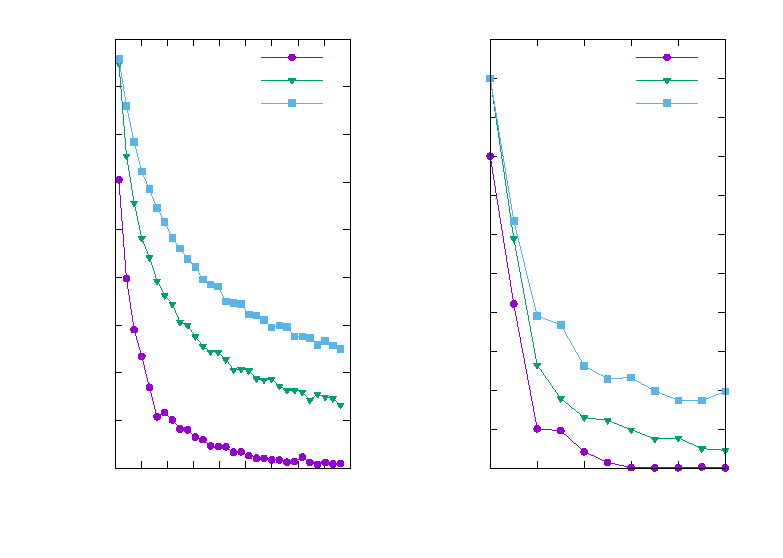
\includegraphics[width={361.00bp},height={253.00bp}]{zigzag-width-strangth}}%
    \gplfronttext
  \end{picture}%
\endgroup

      \caption{(الف) رسانایی در مقابل طول نوار با عرض های مختلف (از نظر تعداد سلول های واحد در یک ابرسلول) و قدرت بی نظمی ثابت $V_d=2\;eV$. (ب) رسانایی در برابر استحکام بی نظمی برای نوارهای زیگزاگ با بی نظمی که در هر دو لبه به طول $876.68$\AA توزیع شده است.}
      \label{zigzag-width-strangth}
    \end{figure*}
    
که در آن و I یک کمیت بی نهایت کوچک مثبت و به ترتیب هویت ما را نشان می دهد. چگالی الکترونی فضایی حالتها در کل محل نانوروبان بوروفن صندلی با یک مکان پراکندگی در لبه بالایی با V=0،1،2،5 در وسط نانوروبان ترسیم شده است. شکل 6.

\begin{figure*}[!ht]
    \centering
    % GNUPLOT: LaTeX picture with Postscript
\begingroup
  % Encoding inside the plot.  In the header of your document, this encoding
  % should to defined, e.g., by using
  % \usepackage[cp1252,<other encodings>]{inputenc}
  % \inputencoding{cp1252}%
  \makeatletter
  \providecommand\color[2][]{%
    \GenericError{(gnuplot) \space\space\space\@spaces}{%
      Package color not loaded in conjunction with
      terminal option `colourtext'%
    }{See the gnuplot documentation for explanation.%
    }{Either use 'blacktext' in gnuplot or load the package
      color.sty in LaTeX.}%
    \renewcommand\color[2][]{}%
  }%
  \providecommand\includegraphics[2][]{%
    \GenericError{(gnuplot) \space\space\space\@spaces}{%
      Package graphicx or graphics not loaded%
    }{See the gnuplot documentation for explanation.%
    }{The gnuplot epslatex terminal needs graphicx.sty or graphics.sty.}%
    \renewcommand\includegraphics[2][]{}%
  }%
  \providecommand\rotatebox[2]{#2}%
  \@ifundefined{ifGPcolor}{%
    \newif\ifGPcolor
    \GPcolorfalse
  }{}%
  \@ifundefined{ifGPblacktext}{%
    \newif\ifGPblacktext
    \GPblacktexttrue
  }{}%
  % define a \g@addto@macro without @ in the name:
  \let\gplgaddtomacro\g@addto@macro
  % define empty templates for all commands taking text:
  \gdef\gplbacktext{}%
  \gdef\gplfronttext{}%
  \makeatother
  \ifGPblacktext
    % no textcolor at all
    \def\colorrgb#1{}%
    \def\colorgray#1{}%
  \else
    % gray or color?
    \ifGPcolor
      \def\colorrgb#1{\color[rgb]{#1}}%
      \def\colorgray#1{\color[gray]{#1}}%
      \expandafter\def\csname LTw\endcsname{\color{white}}%
      \expandafter\def\csname LTb\endcsname{\color{black}}%
      \expandafter\def\csname LTa\endcsname{\color{black}}%
      \expandafter\def\csname LT0\endcsname{\color[rgb]{1,0,0}}%
      \expandafter\def\csname LT1\endcsname{\color[rgb]{0,1,0}}%
      \expandafter\def\csname LT2\endcsname{\color[rgb]{0,0,1}}%
      \expandafter\def\csname LT3\endcsname{\color[rgb]{1,0,1}}%
      \expandafter\def\csname LT4\endcsname{\color[rgb]{0,1,1}}%
      \expandafter\def\csname LT5\endcsname{\color[rgb]{1,1,0}}%
      \expandafter\def\csname LT6\endcsname{\color[rgb]{0,0,0}}%
      \expandafter\def\csname LT7\endcsname{\color[rgb]{1,0.3,0}}%
      \expandafter\def\csname LT8\endcsname{\color[rgb]{0.5,0.5,0.5}}%
    \else
      % gray
      \def\colorrgb#1{\color{black}}%
      \def\colorgray#1{\color[gray]{#1}}%
      \expandafter\def\csname LTw\endcsname{\color{white}}%
      \expandafter\def\csname LTb\endcsname{\color{black}}%
      \expandafter\def\csname LTa\endcsname{\color{black}}%
      \expandafter\def\csname LT0\endcsname{\color{black}}%
      \expandafter\def\csname LT1\endcsname{\color{black}}%
      \expandafter\def\csname LT2\endcsname{\color{black}}%
      \expandafter\def\csname LT3\endcsname{\color{black}}%
      \expandafter\def\csname LT4\endcsname{\color{black}}%
      \expandafter\def\csname LT5\endcsname{\color{black}}%
      \expandafter\def\csname LT6\endcsname{\color{black}}%
      \expandafter\def\csname LT7\endcsname{\color{black}}%
      \expandafter\def\csname LT8\endcsname{\color{black}}%
    \fi
  \fi
    \setlength{\unitlength}{0.0500bp}%
    \ifx\gptboxheight\undefined%
      \newlength{\gptboxheight}%
      \newlength{\gptboxwidth}%
      \newsavebox{\gptboxtext}%
    \fi%
    \setlength{\fboxrule}{0.5pt}%
    \setlength{\fboxsep}{1pt}%
\begin{picture}(7200.00,5040.00)%
    \gplgaddtomacro\gplbacktext{%
      \csname LTb\endcsname%%
      \put(814,704){\makebox(0,0)[r]{\strut{}$0$}}%
      \put(814,1390){\makebox(0,0)[r]{\strut{}$0.5$}}%
      \put(814,2076){\makebox(0,0)[r]{\strut{}$1$}}%
      \put(814,2762){\makebox(0,0)[r]{\strut{}$1.5$}}%
      \put(814,3447){\makebox(0,0)[r]{\strut{}$2$}}%
      \put(814,4133){\makebox(0,0)[r]{\strut{}$2.5$}}%
      \put(814,4819){\makebox(0,0)[r]{\strut{}$3$}}%
      \put(946,484){\makebox(0,0){\strut{}$0$}}%
      \put(1322,484){\makebox(0,0){\strut{}$5$}}%
      \put(1698,484){\makebox(0,0){\strut{}$10$}}%
      \put(2075,484){\makebox(0,0){\strut{}$15$}}%
      \put(2451,484){\makebox(0,0){\strut{}$20$}}%
      \put(2827,484){\makebox(0,0){\strut{}$25$}}%
      \put(3203,484){\makebox(0,0){\strut{}$30$}}%
      \put(1172,4613){\makebox(0,0)[l]{\strut{}(a)}}%
    }%
    \gplgaddtomacro\gplfronttext{%
      \csname LTb\endcsname%%
      \put(209,2761){\rotatebox{-270}{\makebox(0,0){\strut{}$G/G_0$}}}%
      \put(2074,154){\makebox(0,0){\strut{}Lenght(nm)$*10^{1}$}}%
      \csname LTb\endcsname%%
      \put(2216,4646){\makebox(0,0)[r]{\strut{}W=4}}%
      \csname LTb\endcsname%%
      \put(2216,4426){\makebox(0,0)[r]{\strut{}W=6}}%
      \csname LTb\endcsname%%
      \put(2216,4206){\makebox(0,0)[r]{\strut{}W=8}}%
    }%
    \gplgaddtomacro\gplbacktext{%
      \csname LTb\endcsname%%
      \put(4414,704){\makebox(0,0)[r]{\strut{}$0$}}%
      \put(4414,1390){\makebox(0,0)[r]{\strut{}$0.5$}}%
      \put(4414,2076){\makebox(0,0)[r]{\strut{}$1$}}%
      \put(4414,2762){\makebox(0,0)[r]{\strut{}$1.5$}}%
      \put(4414,3447){\makebox(0,0)[r]{\strut{}$2$}}%
      \put(4414,4133){\makebox(0,0)[r]{\strut{}$2.5$}}%
      \put(4414,4819){\makebox(0,0)[r]{\strut{}$3$}}%
      \put(4546,484){\makebox(0,0){\strut{}$0$}}%
      \put(4922,484){\makebox(0,0){\strut{}$0.5$}}%
      \put(5298,484){\makebox(0,0){\strut{}$1$}}%
      \put(5675,484){\makebox(0,0){\strut{}$1.5$}}%
      \put(6051,484){\makebox(0,0){\strut{}$2$}}%
      \put(6427,484){\makebox(0,0){\strut{}$2.5$}}%
      \put(6803,484){\makebox(0,0){\strut{}$3$}}%
      \put(4772,4613){\makebox(0,0)[l]{\strut{}(b)}}%
    }%
    \gplgaddtomacro\gplfronttext{%
      \csname LTb\endcsname%%
      \put(3809,2761){\rotatebox{-270}{\makebox(0,0){\strut{}$G/G_0$}}}%
      \put(5674,154){\makebox(0,0){\strut{}$V_d(eV)$}}%
      \csname LTb\endcsname%%
      \put(5816,4646){\makebox(0,0)[r]{\strut{}W=4}}%
      \csname LTb\endcsname%%
      \put(5816,4426){\makebox(0,0)[r]{\strut{}W=6}}%
      \csname LTb\endcsname%%
      \put(5816,4206){\makebox(0,0)[r]{\strut{}W=8}}%
    }%
    \gplbacktext
    \put(0,0){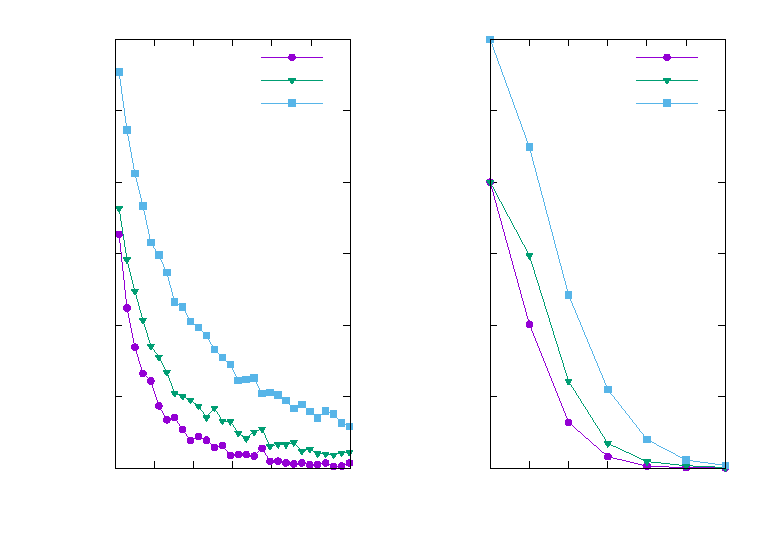
\includegraphics[width={360.00bp},height={252.00bp}]{armchair-width-strangth}}%
    \gplfronttext
  \end{picture}%
\endgroup

    \caption{(الف) رسانایی در مقابل طول روبان صندلی صندلی با عرض های مختلف (از نظر تعداد سلول های واحد در یک سوپرسل) و قدرت بی نظمی ثابت $V_d=1\;eV$. (ب) رسانایی در مقابل استحکام بی نظمی برای روبان های صندلی صندلی با بی نظمی که در هر دو لبه به طول $758.81$\AA توزیع شده است.}
    \label{armchair-width-strangth}
  \end{figure*}
  
% این فرآیند تا tn، ̃ tn ≤ δ تکرار می شود و δ به طور دلخواه کوچک است. باید توجه داشته باشیم که بعد ماتریس تعداد اتم های داخل سوپرسل است. با احتساب نمونه به عنوان بخشی از سرب سمت راست، لایه به لایه (از l=M تا l=2)، توابع سبز سطح جدید به صورت زیر یافت می شوند:
% در اینجا L (R) توابع خود انرژی هستند که اتلاف ناشی از برهمکنش با سمت چپ (راست) سازه را در نظر می گیرند.
هامیلتونی کل نانوروبان به شکل یک ماتریس سه قطری است که در آن عناصر روی شکل 7. در انرژی مربوط به اوج LDOS نزدیک به انرژی فرمی، چگالی الکترونی فضایی حالتها در کل محل نانوروبان بوروفن زیگزاگ با یک مکان خالی در لبه بالایی بدون خالی، یک جای خالی و دو جای خالی در وسط نانو نوار رسم شده است. شکل 8. 
% (الف) رسانایی نانوروبان های صندلی صندلی با عرض\AA 10.24 و طول 74.36\AA Å، با جاهای خالی واقع در لبه بالایی سوپرسل میانی نانوروبان. (ب) چگالی الکترونی حالتها در نزدیکترین محل همسایه جاهای خالی واقع شده مشابه (الف). 
مورب اصلی ماتریس هامیلتونی هستند که با (Hl,l) نشان داده می شوند و عناصر روی دو قطر دیگر ماتریس برهمکنش مجاور دو ابرسلول به صورت (Hl,l+1) هستند. با استفاده از انرژی های خود با ابعاد مشابه با ماتریس کل هامیلتونی، تابع گرین کل نانوروبان را می توان به دست آورد. این تابع کل سبز میتواند به ویژگیهای محلی در هر نقطه از نانوروبان، مانند LDOS منجر شود (شکل 9).


\subsection{اختلال ضعیف محلی سازی اندرسون در نانونوارهای بورفین}
پدیده ای است که ناشی از تداخل امواج منتشر شده از مسیرهای متعدد است که در انواع سیستم های موجی قابل مشاهده است [61-65]. درک کامل محلیسازی اندرسون امکانپذیر نخواهد بود مگر اینکه عواملی را کنترل کنیم که بر آن تأثیر میگذارند، از جمله برهمکنشهای بین ذرهای، بعد، تقارن معکوس زمانی، و ماهیت میکروسکوپی اختلال. یکی از مناسبترین و قابل کنترلترین نمونههای این امر میتواند سیستمهای کوانتومی اتمهای Ultracold باشد که منجر به درک عمیق محلیسازی اندرسون میشود [66]. مکان یابی اندرسون در فیزیک حالت جامد بسیار جالب است زیرا پیش بینی می کند که یک الکترون ممکن است در یک شبکه بی نظم بی حرکت شود [67]. از قضیه بلوخ، میدانیم که در یک سیستم مکانیکی کوانتومی با یک همیلتونی تناوبی فضایی، حالتهای ویژه تک ذرهای در سراسر فضا گسترش یافتهاند. وجود اختلال ایستا تقارن انتقالی کریستالی و هامیلتونی را می شکند و در نتیجه احتمال حالت های ویژه را افزایش می دهد که به صورت تصاعدی موضعی می شوند [68]. به طور کلی، هر چه میزان اختلال بیشتر باشد، تعداد حالتهای ویژه موضعی بیشتر میشود و در برخی موارد، زمانی که اختلال به اندازه کافی بزرگ است، همه حالتهای گسترشیافته را به حالتهای موضعی تبدیل میکند و باعث انتقال اندرسون میشود. حالتهای ویژه گسترده یا موضعی مربوط به حضور یا عدم وجود ذرات برای انتقال در مقیاس طول ماکروسکوپی است. (حالتهای گسترشیافته منجر به جابجایی مربع میانگین میشود که با گذشت زمان برای مدت طولانی رشد میکند، در حالی که حالتهای موضعی رشد میکنند.) بنابراین، محلیسازی اندرسون میتواند پدیدههای انتقال، از جمله انتقال عایق فلزی در نیمهرساناها را توضیح دهد.

در اینجا، از آنجایی که با یک سیستم شبه یک بعدی سروکار داریم، ناخالصی ها تنها در لبه های بالایی و پایینی نانوروبان ها با اختصاص یک متغیر تصادفی نامرتبط به هر یک از آنها توزیع می شوند. ناخالصی ها در امتداد لبه های نانوروبان توزیع می شوند و قدرت بالقوه آنها به طور تصادفی از محدوده $[-V_d, V_d]$ انتخاب می شود. همانطور که در شکل 10 مشاهده می شود، اگرچه پتانسیل های بسیار ضعیف رسانایی را کاهش می دهند، اما نمی توانند باعث محلی سازی اندرسون شوند. همانطور که قدرت پتانسیل افزایش می یابد، واضح است که محلی سازی در انرژی هایی در حدود $-0.5 eV$ زمانی که $V_d = 2 eV$ رخ می دهد. به عبارت دیگر، برای قدرت پتانسیل بسیار ضعیف، طول محلی سازی بسیار طولانی است. این را می توان با این واقعیت توضیح داد که در یک سیستم یک بعدی بی نهایت، حتی یک اختلال بسیار ضعیف می تواند تداخل سازنده را مختل کند و باعث رسانایی صفر شود. طول محلیسازی بهعنوان طولی تعریف میشود که در آن همه حالتهای ویژه بلوخ بهصورت فضایی گسترشیافته به حالتهای موضعی تغییر میکنند و در نتیجه رسانایی صفر میشود. همانطور که انتظار می رود، با افزایش طول نوار با قدرت پتانسیل $2 eV$ در لبه ها، رسانایی احتمالاً به طور تصاعدی کاهش می یابد. شکل 12.a یک رسانایی در انرژی فرمی را با میانگین بیش از 1000 پیکربندی مختلف از انتخاب های تصادفی پتانسیل در لبه ها برای عرض های مختلف ZBNR نشان می دهد، که نشان دهنده کاهش نمایی در رسانایی است. در ZBNRها، تعداد کانالهای رسانایی در اطراف انرژی فرمی به عرض نانوروبانها بستگی دارد، که تفاوت بین رسانایی نانوروبانهایی با طولهای کوچک با عرضهای مختلف را در تضاد واضح با مورد گرافن توضیح میدهد. علاوه بر این، طول طول محلی سازی اندرسون در ZBNR ها (تقریباً 1801800 نانومتر برای عرض سلول های 4-8 واحد) بسیار بیشتر از ZGNR ها است (تقریباً 200-800 آنگستروم که با آنچه توسط Li و همکاران گزارش شده مطابقت دارد). [69] انگرافن). همانطور که مشاهده می شود، هر چه قدرت اختلال بیشتر باشد، طول محلی سازی کوتاهتر به دست می آید. رسانایی ABNR ها با عرض 10.24 Å و طول نانوروبان 758.81 Å در شکل 11 نشان داده شده است. برخلاف ZBNR ها، حتی قدرت بی نظمی بسیار ضعیف نیز ممکن است اثرات قابل توجهی بر رسانایی داشته باشد، با طول محلی سازی بسیار کوتاه تر از طول محلی سازی مشاهده شده در ZBNR ها شکل 13، تغییر رسانایی در ABNRها را به عنوان تابعی از طول شکل 13.a و قدرت بالقوه شکل 13.b در انرژی انرژی فرمی، که از طریق میانگین بیش از 1000 پیکربندی مختلف اختلال لبه محاسبه شده است، نشان می دهد. هر دو شکل نشان دهنده کاهش نمایی رسانایی زمانی است که طول (یا قدرت پتانسیل) در ABNR ها افزایش می یابد. همانطور که انتظار می رود، افزایش در تعداد کانال های رسانایی زمانی مشاهده می شود که عرض ABNR ها افزایش می یابد، که از نظر کیفی مشابه آنچه برای ZBNR به دست آمده است. دلیل فیزیکی پشت تاثیر بیشتر اختلال ضعیف بر هدایت ABNR ها در مقایسه با ZBNR ها را می توان با سرعت بالاتر سرعت گروه الکترونی در ZNBR ها در مقایسه با ABNR ها در محدوده انرژی فرمی درک کرد.

\begin{figure*}
\resizebox{0.95\textwidth}{!}{\includegraphics{./figures/Shematic3.png}}
\caption{به صورت شماتیک ساختار یک دریچه اسپینی مبتنی بر $\beta$-borophene را با لیدهای مغناطیسی نشان می دهد، که در آن بردارهای مغناطیسی دو لید می توانند زاویه نسبی $\theta$ داشته باشند. مغناطیسی شدن لیدها ناشی از زیرلایه مغناطیسی است که روی آن قرار می گیرند که می توان آن را به صورت تجربی کنترل کرد. در قسمت بالای شکل، بوروفن نانوروبان با لبه های صندلی راحتی و در قسمت پایین شکل، نانوروبان بوروفن زیگزاگ به تصویر کشیده شده است. سلول واحد بوروفن با اتم‌های بور که در یک بورفن لبه زیگزاگ برچسب‌گذاری شده‌اند در جدول\ref{tbl:hoppingtable} نشان داده شده است، جایی که انرژی‌های موجود در محل و پارامترهای جهش اتم‌ها آورده شده است.}
  \label{fig:model}
\end{figure*}
    
\begin{figure*}[ht]
\centering
\resizebox{0.45\textwidth}{!}{\input{./figures/Armchair-Antiparallel-conductance-revise.tex}}
\resizebox{0.45\textwidth}{!}{% GNUPLOT: LaTeX picture with Postscript
\begin{latin}
\begingroup
  % Encoding inside the plot.  In the header of your document, this encoding
  % should to defined, e.g., by using
  % \usepackage[cp1252,<other encodings>]{inputenc}
  % \inputencoding{cp1252}%
  \makeatletter
  \providecommand\color[2][]{%
    \GenericError{(gnuplot) \space\space\space\@spaces}{%
      Package color not loaded in conjunction with
      terminal option `colourtext'%
    }{See the gnuplot documentation for explanation.%
    }{Either use 'blacktext' in gnuplot or load the package
      color.sty in LaTeX.}%
    \renewcommand\color[2][]{}%
  }%
  \providecommand\includegraphics[2][]{%
    \GenericError{(gnuplot) \space\space\space\@spaces}{%
      Package graphicx or graphics not loaded%
    }{See the gnuplot documentation for explanation.%
    }{The gnuplot epslatex terminal needs graphicx.sty or graphics.sty.}%
    \renewcommand\includegraphics[2][]{}%
  }%
  \providecommand\rotatebox[2]{#2}%
  \@ifundefined{ifGPcolor}{%
    \newif\ifGPcolor
    \GPcolorfalse
  }{}%
  \@ifundefined{ifGPblacktext}{%
    \newif\ifGPblacktext
    \GPblacktexttrue
  }{}%
  % define a \g@addto@macro without @ in the name:
  \let\gplgaddtomacro\g@addto@macro
  % define empty templates for all commands taking text:
  \gdef\gplbacktext{}%
  \gdef\gplfronttext{}%
  \makeatother
  \ifGPblacktext
    % no textcolor at all
    \def\colorrgb#1{}%
    \def\colorgray#1{}%
  \else
    % gray or color?
    \ifGPcolor
      \def\colorrgb#1{\color[rgb]{#1}}%
      \def\colorgray#1{\color[gray]{#1}}%
      \expandafter\def\csname LTw\endcsname{\color{white}}%
      \expandafter\def\csname LTb\endcsname{\color{black}}%
      \expandafter\def\csname LTa\endcsname{\color{black}}%
      \expandafter\def\csname LT0\endcsname{\color[rgb]{1,0,0}}%
      \expandafter\def\csname LT1\endcsname{\color[rgb]{0,1,0}}%
      \expandafter\def\csname LT2\endcsname{\color[rgb]{0,0,1}}%
      \expandafter\def\csname LT3\endcsname{\color[rgb]{1,0,1}}%
      \expandafter\def\csname LT4\endcsname{\color[rgb]{0,1,1}}%
      \expandafter\def\csname LT5\endcsname{\color[rgb]{1,1,0}}%
      \expandafter\def\csname LT6\endcsname{\color[rgb]{0,0,0}}%
      \expandafter\def\csname LT7\endcsname{\color[rgb]{1,0.3,0}}%
      \expandafter\def\csname LT8\endcsname{\color[rgb]{0.5,0.5,0.5}}%
    \else
      % gray
      \def\colorrgb#1{\color{black}}%
      \def\colorgray#1{\color[gray]{#1}}%
      \expandafter\def\csname LTw\endcsname{\color{white}}%
      \expandafter\def\csname LTb\endcsname{\color{black}}%
      \expandafter\def\csname LTa\endcsname{\color{black}}%
      \expandafter\def\csname LT0\endcsname{\color{black}}%
      \expandafter\def\csname LT1\endcsname{\color{black}}%
      \expandafter\def\csname LT2\endcsname{\color{black}}%
      \expandafter\def\csname LT3\endcsname{\color{black}}%
      \expandafter\def\csname LT4\endcsname{\color{black}}%
      \expandafter\def\csname LT5\endcsname{\color{black}}%
      \expandafter\def\csname LT6\endcsname{\color{black}}%
      \expandafter\def\csname LT7\endcsname{\color{black}}%
      \expandafter\def\csname LT8\endcsname{\color{black}}%
    \fi
  \fi
    \setlength{\unitlength}{0.0500bp}%
    \ifx\gptboxheight\undefined%
      \newlength{\gptboxheight}%
      \newlength{\gptboxwidth}%
      \newsavebox{\gptboxtext}%
    \fi%
    \setlength{\fboxrule}{0.5pt}%
    \setlength{\fboxsep}{1pt}%
\begin{picture}(7200.00,5040.00)%
    \gplgaddtomacro\gplbacktext{%
      \csname LTb\endcsname%%
      \put(900,4200){\makebox(0,0)[r]{\strut{}$B$}}%
      \put(550,704){\makebox(0,0)[r]{\strut{}$0$}}%
      \put(550,1112){\makebox(0,0)[r]{\strut{}$1$}}%
      \put(550,1521){\makebox(0,0)[r]{\strut{}$2$}}%
      \put(550,1929){\makebox(0,0)[r]{\strut{}$3$}}%
      \put(550,2337){\makebox(0,0)[r]{\strut{}$4$}}%
      \put(550,2746){\makebox(0,0)[r]{\strut{}$5$}}%
      \put(550,3154){\makebox(0,0)[r]{\strut{}$6$}}%
      \put(550,3562){\makebox(0,0)[r]{\strut{}$7$}}%
      \put(550,3971){\makebox(0,0)[r]{\strut{}$8$}}%
      \put(550,4379){\makebox(0,0)[r]{\strut{}$9$}}%
      \put(682,484){\makebox(0,0){\strut{}$-4$}}%
      \put(1447,484){\makebox(0,0){\strut{}$-3$}}%
      \put(2212,484){\makebox(0,0){\strut{}$-2$}}%
      \put(2977,484){\makebox(0,0){\strut{}$-1$}}%
      \put(3743,484){\makebox(0,0){\strut{}$0$}}%
      \put(4508,484){\makebox(0,0){\strut{}$1$}}%
      \put(5273,484){\makebox(0,0){\strut{}$2$}}%
      \put(6038,484){\makebox(0,0){\strut{}$3$}}%
      \put(6803,484){\makebox(0,0){\strut{}$4$}}%
    }%
    \gplgaddtomacro\gplfronttext{%
      \csname LTb\endcsname%%
      \put(209,2541){\rotatebox{-270}{\makebox(0,0){\strut{}$G(e^2/h)$}}}%
      \put(3742,154){\makebox(0,0){\strut{}$E(eV)$}}%
      \csname LTb\endcsname%%
      \put(2522,4206){\makebox(0,0)[r]{\strut{}$M=0$}}%
      \csname LTb\endcsname%%
      \put(2522,3986){\makebox(0,0)[r]{\strut{}$M=0.05$}}%
      \csname LTb\endcsname%%
      \put(4169,4206){\makebox(0,0)[r]{\strut{}$M=0.1$}}%
      \csname LTb\endcsname%%
      \put(4169,3986){\makebox(0,0)[r]{\strut{}$M=0.2$}}%
      \csname LTb\endcsname%%
      \put(5816,4206){\makebox(0,0)[r]{\strut{}$M=0.3$}}%
      \csname LTb\endcsname%%
      \put(3742,4709){\makebox(0,0){\strut{}Parallel}}%
    }%
    \gplbacktext
    \put(0,0){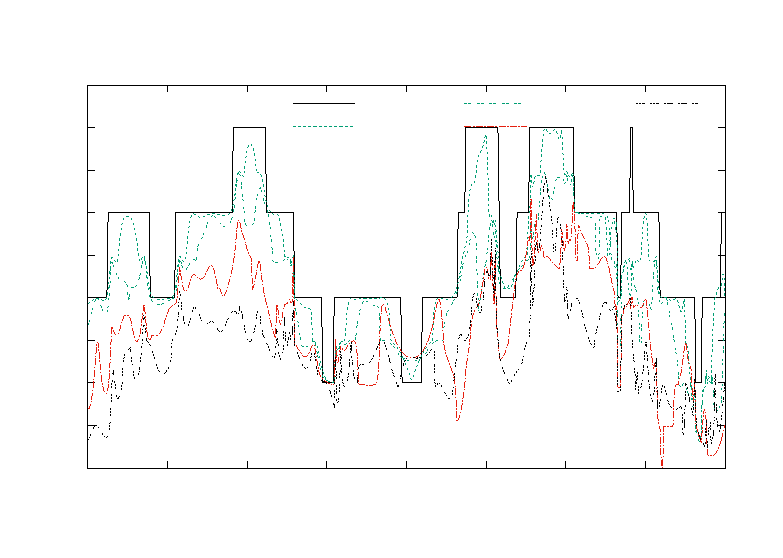
\includegraphics[width={360.00bp},height={252.00bp}]{armchair-parallel-conductance-revise}}%
    \gplfronttext
  \end{picture}%
\endgroup
\end{latin}}
\resizebox{0.45\textwidth}{!}{% GNUPLOT: LaTeX picture with Postscript
\begingroup
  % Encoding inside the plot.  In the header of your document, this encoding
  % should to defined, e.g., by using
  % \usepackage[cp1252,<other encodings>]{inputenc}
  % \inputencoding{cp1252}%
  \makeatletter
  \providecommand\color[2][]{%
    \GenericError{(gnuplot) \space\space\space\@spaces}{%
      Package color not loaded in conjunction with
      terminal option `colourtext'%
    }{See the gnuplot documentation for explanation.%
    }{Either use 'blacktext' in gnuplot or load the package
      color.sty in LaTeX.}%
    \renewcommand\color[2][]{}%
  }%
  \providecommand\includegraphics[2][]{%
    \GenericError{(gnuplot) \space\space\space\@spaces}{%
      Package graphicx or graphics not loaded%
    }{See the gnuplot documentation for explanation.%
    }{The gnuplot epslatex terminal needs graphicx.sty or graphics.sty.}%
    \renewcommand\includegraphics[2][]{}%
  }%
  \providecommand\rotatebox[2]{#2}%
  \@ifundefined{ifGPcolor}{%
    \newif\ifGPcolor
    \GPcolorfalse
  }{}%
  \@ifundefined{ifGPblacktext}{%
    \newif\ifGPblacktext
    \GPblacktexttrue
  }{}%
  % define a \g@addto@macro without @ in the name:
  \let\gplgaddtomacro\g@addto@macro
  % define empty templates for all commands taking text:
  \gdef\gplbacktext{}%
  \gdef\gplfronttext{}%
  \makeatother
  \ifGPblacktext
    % no textcolor at all
    \def\colorrgb#1{}%
    \def\colorgray#1{}%
  \else
    % gray or color?
    \ifGPcolor
      \def\colorrgb#1{\color[rgb]{#1}}%
      \def\colorgray#1{\color[gray]{#1}}%
      \expandafter\def\csname LTw\endcsname{\color{white}}%
      \expandafter\def\csname LTb\endcsname{\color{black}}%
      \expandafter\def\csname LTa\endcsname{\color{black}}%
      \expandafter\def\csname LT0\endcsname{\color[rgb]{1,0,0}}%
      \expandafter\def\csname LT1\endcsname{\color[rgb]{0,1,0}}%
      \expandafter\def\csname LT2\endcsname{\color[rgb]{0,0,1}}%
      \expandafter\def\csname LT3\endcsname{\color[rgb]{1,0,1}}%
      \expandafter\def\csname LT4\endcsname{\color[rgb]{0,1,1}}%
      \expandafter\def\csname LT5\endcsname{\color[rgb]{1,1,0}}%
      \expandafter\def\csname LT6\endcsname{\color[rgb]{0,0,0}}%
      \expandafter\def\csname LT7\endcsname{\color[rgb]{1,0.3,0}}%
      \expandafter\def\csname LT8\endcsname{\color[rgb]{0.5,0.5,0.5}}%
    \else
      % gray
      \def\colorrgb#1{\color{black}}%
      \def\colorgray#1{\color[gray]{#1}}%
      \expandafter\def\csname LTw\endcsname{\color{white}}%
      \expandafter\def\csname LTb\endcsname{\color{black}}%
      \expandafter\def\csname LTa\endcsname{\color{black}}%
      \expandafter\def\csname LT0\endcsname{\color{black}}%
      \expandafter\def\csname LT1\endcsname{\color{black}}%
      \expandafter\def\csname LT2\endcsname{\color{black}}%
      \expandafter\def\csname LT3\endcsname{\color{black}}%
      \expandafter\def\csname LT4\endcsname{\color{black}}%
      \expandafter\def\csname LT5\endcsname{\color{black}}%
      \expandafter\def\csname LT6\endcsname{\color{black}}%
      \expandafter\def\csname LT7\endcsname{\color{black}}%
      \expandafter\def\csname LT8\endcsname{\color{black}}%
    \fi
  \fi
    \setlength{\unitlength}{0.0500bp}%
    \ifx\gptboxheight\undefined%
      \newlength{\gptboxheight}%
      \newlength{\gptboxwidth}%
      \newsavebox{\gptboxtext}%
    \fi%
    \setlength{\fboxrule}{0.5pt}%
    \setlength{\fboxsep}{1pt}%
\begin{picture}(7200.00,5040.00)%
    \gplgaddtomacro\gplbacktext{%
      \csname LTb\endcsname%%
      \put(1000,4200){\makebox(0,0)[r]{\strut{}$C$}}%
      \put(682,704){\makebox(0,0)[r]{\strut{}$2$}}%
      \put(682,1163){\makebox(0,0)[r]{\strut{}$4$}}%
      \put(682,1623){\makebox(0,0)[r]{\strut{}$6$}}%
      \put(682,2082){\makebox(0,0)[r]{\strut{}$8$}}%
      \put(682,2542){\makebox(0,0)[r]{\strut{}$10$}}%
      \put(682,3001){\makebox(0,0)[r]{\strut{}$12$}}%
      \put(682,3460){\makebox(0,0)[r]{\strut{}$14$}}%
      \put(682,3920){\makebox(0,0)[r]{\strut{}$16$}}%
      \put(682,4379){\makebox(0,0)[r]{\strut{}$18$}}%
      \put(814,484){\makebox(0,0){\strut{}$-4$}}%
      \put(1563,484){\makebox(0,0){\strut{}$-3$}}%
      \put(2311,484){\makebox(0,0){\strut{}$-2$}}%
      \put(3060,484){\makebox(0,0){\strut{}$-1$}}%
      \put(3809,484){\makebox(0,0){\strut{}$0$}}%
      \put(4557,484){\makebox(0,0){\strut{}$1$}}%
      \put(5306,484){\makebox(0,0){\strut{}$2$}}%
      \put(6054,484){\makebox(0,0){\strut{}$3$}}%
      \put(6803,484){\makebox(0,0){\strut{}$4$}}%
    }%
    \gplgaddtomacro\gplfronttext{%
      \csname LTb\endcsname%%
      \put(209,2541){\rotatebox{-270}{\makebox(0,0){\strut{}$G(e^2/h)$}}}%
      \put(3808,154){\makebox(0,0){\strut{}$E(eV)$}}%
      \csname LTb\endcsname%%
      \put(2522,4206){\makebox(0,0)[r]{\strut{}$M=0$}}%
      \csname LTb\endcsname%%
      \put(2522,3986){\makebox(0,0)[r]{\strut{}$M=0.05$}}%
      \csname LTb\endcsname%%
      \put(4169,4206){\makebox(0,0)[r]{\strut{}$M=0.1$}}%
      \csname LTb\endcsname%%
      \put(4169,3986){\makebox(0,0)[r]{\strut{}$M=0.2$}}%
      \csname LTb\endcsname%%
      \put(5816,4206){\makebox(0,0)[r]{\strut{}$M=0.3$}}%
      \csname LTb\endcsname%%
      \put(3808,4709){\makebox(0,0){\strut{}AntiParallel}}%
    }%
    \gplbacktext
    \put(0,0){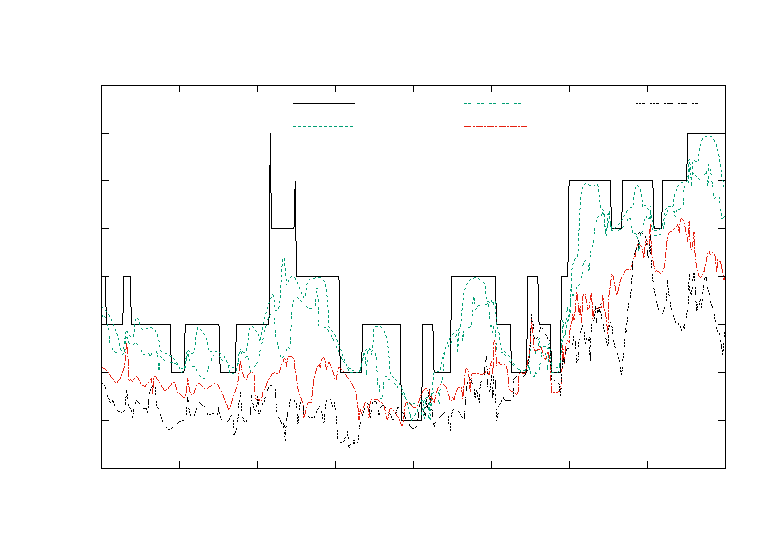
\includegraphics[width={360.00bp},height={252.00bp}]{zigzag-antiparallel-conductance-revise}}%
    \gplfronttext
  \end{picture}%
\endgroup
}
\resizebox{0.45\textwidth}{!}{% GNUPLOT: LaTeX picture with Postscript
\begingroup
  % Encoding inside the plot.  In the header of your document, this encoding
  % should to defined, e.g., by using
  % \usepackage[cp1252,<other encodings>]{inputenc}
  % \inputencoding{cp1252}%
  \makeatletter
  \providecommand\color[2][]{%
    \GenericError{(gnuplot) \space\space\space\@spaces}{%
      Package color not loaded in conjunction with
      terminal option `colourtext'%
    }{See the gnuplot documentation for explanation.%
    }{Either use 'blacktext' in gnuplot or load the package
      color.sty in LaTeX.}%
    \renewcommand\color[2][]{}%
  }%
  \providecommand\includegraphics[2][]{%
    \GenericError{(gnuplot) \space\space\space\@spaces}{%
      Package graphicx or graphics not loaded%
    }{See the gnuplot documentation for explanation.%
    }{The gnuplot epslatex terminal needs graphicx.sty or graphics.sty.}%
    \renewcommand\includegraphics[2][]{}%
  }%
  \providecommand\rotatebox[2]{#2}%
  \@ifundefined{ifGPcolor}{%
    \newif\ifGPcolor
    \GPcolorfalse
  }{}%
  \@ifundefined{ifGPblacktext}{%
    \newif\ifGPblacktext
    \GPblacktexttrue
  }{}%
  % define a \g@addto@macro without @ in the name:
  \let\gplgaddtomacro\g@addto@macro
  % define empty templates for all commands taking text:
  \gdef\gplbacktext{}%
  \gdef\gplfronttext{}%
  \makeatother
  \ifGPblacktext
    % no textcolor at all
    \def\colorrgb#1{}%
    \def\colorgray#1{}%
  \else
    % gray or color?
    \ifGPcolor
      \def\colorrgb#1{\color[rgb]{#1}}%
      \def\colorgray#1{\color[gray]{#1}}%
      \expandafter\def\csname LTw\endcsname{\color{white}}%
      \expandafter\def\csname LTb\endcsname{\color{black}}%
      \expandafter\def\csname LTa\endcsname{\color{black}}%
      \expandafter\def\csname LT0\endcsname{\color[rgb]{1,0,0}}%
      \expandafter\def\csname LT1\endcsname{\color[rgb]{0,1,0}}%
      \expandafter\def\csname LT2\endcsname{\color[rgb]{0,0,1}}%
      \expandafter\def\csname LT3\endcsname{\color[rgb]{1,0,1}}%
      \expandafter\def\csname LT4\endcsname{\color[rgb]{0,1,1}}%
      \expandafter\def\csname LT5\endcsname{\color[rgb]{1,1,0}}%
      \expandafter\def\csname LT6\endcsname{\color[rgb]{0,0,0}}%
      \expandafter\def\csname LT7\endcsname{\color[rgb]{1,0.3,0}}%
      \expandafter\def\csname LT8\endcsname{\color[rgb]{0.5,0.5,0.5}}%
    \else
      % gray
      \def\colorrgb#1{\color{black}}%
      \def\colorgray#1{\color[gray]{#1}}%
      \expandafter\def\csname LTw\endcsname{\color{white}}%
      \expandafter\def\csname LTb\endcsname{\color{black}}%
      \expandafter\def\csname LTa\endcsname{\color{black}}%
      \expandafter\def\csname LT0\endcsname{\color{black}}%
      \expandafter\def\csname LT1\endcsname{\color{black}}%
      \expandafter\def\csname LT2\endcsname{\color{black}}%
      \expandafter\def\csname LT3\endcsname{\color{black}}%
      \expandafter\def\csname LT4\endcsname{\color{black}}%
      \expandafter\def\csname LT5\endcsname{\color{black}}%
      \expandafter\def\csname LT6\endcsname{\color{black}}%
      \expandafter\def\csname LT7\endcsname{\color{black}}%
      \expandafter\def\csname LT8\endcsname{\color{black}}%
    \fi
  \fi
    \setlength{\unitlength}{0.0500bp}%
    \ifx\gptboxheight\undefined%
      \newlength{\gptboxheight}%
      \newlength{\gptboxwidth}%
      \newsavebox{\gptboxtext}%
    \fi%
    \setlength{\fboxrule}{0.5pt}%
    \setlength{\fboxsep}{1pt}%
\begin{picture}(7200.00,5040.00)%
    \gplgaddtomacro\gplbacktext{%
      \csname LTb\endcsname%%
      \put(1000,4200){\makebox(0,0)[r]{\strut{}$D$}}%
      \put(682,704){\makebox(0,0)[r]{\strut{}$0$}}%
      \put(682,1112){\makebox(0,0)[r]{\strut{}$2$}}%
      \put(682,1521){\makebox(0,0)[r]{\strut{}$4$}}%
      \put(682,1929){\makebox(0,0)[r]{\strut{}$6$}}%
      \put(682,2337){\makebox(0,0)[r]{\strut{}$8$}}%
      \put(682,2746){\makebox(0,0)[r]{\strut{}$10$}}%
      \put(682,3154){\makebox(0,0)[r]{\strut{}$12$}}%
      \put(682,3562){\makebox(0,0)[r]{\strut{}$14$}}%
      \put(682,3971){\makebox(0,0)[r]{\strut{}$16$}}%
      \put(682,4379){\makebox(0,0)[r]{\strut{}$18$}}%
      \put(814,484){\makebox(0,0){\strut{}$-4$}}%
      \put(1563,484){\makebox(0,0){\strut{}$-3$}}%
      \put(2311,484){\makebox(0,0){\strut{}$-2$}}%
      \put(3060,484){\makebox(0,0){\strut{}$-1$}}%
      \put(3809,484){\makebox(0,0){\strut{}$0$}}%
      \put(4557,484){\makebox(0,0){\strut{}$1$}}%
      \put(5306,484){\makebox(0,0){\strut{}$2$}}%
      \put(6054,484){\makebox(0,0){\strut{}$3$}}%
      \put(6803,484){\makebox(0,0){\strut{}$4$}}%
    }%
    \gplgaddtomacro\gplfronttext{%
      \csname LTb\endcsname%%
      \put(209,2541){\rotatebox{-270}{\makebox(0,0){\strut{}$G(e^2/h)$}}}%
      \put(3808,154){\makebox(0,0){\strut{}$E(eV)$}}%
      \csname LTb\endcsname%%
      \put(2522,4206){\makebox(0,0)[r]{\strut{}$M=0$}}%
      \csname LTb\endcsname%%
      \put(2522,3986){\makebox(0,0)[r]{\strut{}$M=0.05$}}%
      \csname LTb\endcsname%%
      \put(4169,4206){\makebox(0,0)[r]{\strut{}$M=0.1$}}%
      \csname LTb\endcsname%%
      \put(4169,3986){\makebox(0,0)[r]{\strut{}$M=0.2$}}%
      \csname LTb\endcsname%%
      \put(5816,4206){\makebox(0,0)[r]{\strut{}$M=0.3$}}%
      \csname LTb\endcsname%%
      \put(3808,4709){\makebox(0,0){\strut{}Parallel}}%
    }%
    \gplbacktext
    \put(0,0){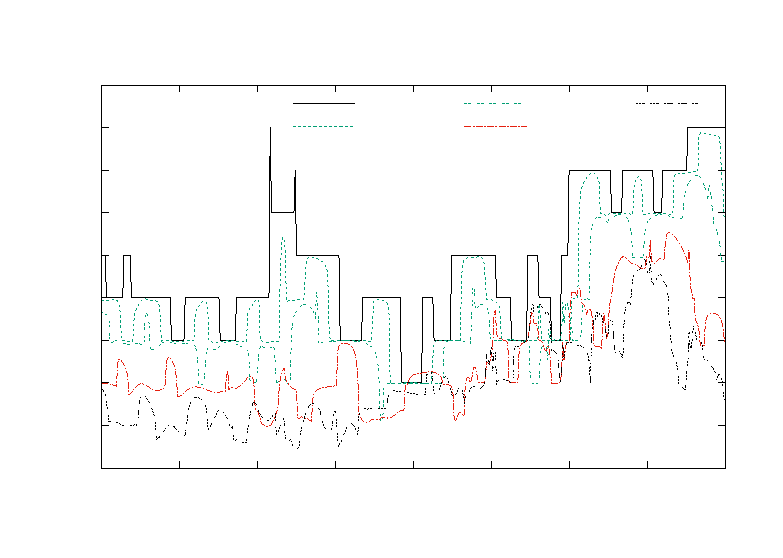
\includegraphics[width={360.00bp},height={252.00bp}]{zigzag-parallel-conductance-revise}}%
    \gplfronttext
  \end{picture}%
\endgroup
}
\caption{الف) پلات بوروفن با لبه صندلی با عرض 4 سلول برای مغناطش متفاوت لیدها در پیکربندی AP. ب) رسم بوروفن با لبه صندلی، و عرض سلول 4 واحد، برای مغناطش متفاوت سرنخ ها در پیکربندی P. ج) نمودار بوروفن با لبه زیگزاگ، با عرض سلول 4 واحد، برای مغناطش متفاوت سرنخ ها در پیکربندی P. د) رسم بوروفن با لبه زیگزاگ و عرض سلول 4 واحد، برای مغناطش متفاوت سرنخ ها در پیکربندی AP.}
\label{fig:conductance}
\end{figure*}
\begin{figure*}[ht]
\centering
\resizebox{0.32\textwidth}{!}{% GNUPLOT: LaTeX picture with Postscript
\begin{latin}
\begingroup
  \makeatletter
  \providecommand\color[2][]{%
    \GenericError{(gnuplot) \space\space\space\@spaces}{%
      Package color not loaded in conjunction with
      terminal option `colourtext'%
    }{See the gnuplot documentation for explanation.%
    }{Either use 'blacktext' in gnuplot or load the package
      color.sty in LaTeX.}%
    \renewcommand\color[2][]{}%
  }%
  \providecommand\includegraphics[2][]{%
    \GenericError{(gnuplot) \space\space\space\@spaces}{%
      Package graphicx or graphics not loaded%
    }{See the gnuplot documentation for explanation.%
    }{The gnuplot epslatex terminal needs graphicx.sty or graphics.sty.}%
    \renewcommand\includegraphics[2][]{}%
  }%
  \providecommand\rotatebox[2]{#2}%
  \@ifundefined{ifGPcolor}{%
    \newif\ifGPcolor
    \GPcolorfalse
  }{}%
  \@ifundefined{ifGPblacktext}{%
    \newif\ifGPblacktext
    \GPblacktexttrue
  }{}%
  % define a \g@addto@macro without @ in the name:
  \let\gplgaddtomacro\g@addto@macro
  % define empty templates for all commands taking text:
  \gdef\gplbacktext{}%
  \gdef\gplfronttext{}%
  \makeatother
  \ifGPblacktext
    % no textcolor at all
    \def\colorrgb#1{}%
    \def\colorgray#1{}%
  \else
    % gray or color?
    \ifGPcolor
      \def\colorrgb#1{\color[rgb]{#1}}%
      \def\colorgray#1{\color[gray]{#1}}%
      \expandafter\def\csname LTw\endcsname{\color{white}}%
      \expandafter\def\csname LTb\endcsname{\color{black}}%
      \expandafter\def\csname LTa\endcsname{\color{black}}%
      \expandafter\def\csname LT0\endcsname{\color[rgb]{1,0,0}}%
      \expandafter\def\csname LT1\endcsname{\color[rgb]{0,1,0}}%
      \expandafter\def\csname LT2\endcsname{\color[rgb]{0,0,1}}%
      \expandafter\def\csname LT3\endcsname{\color[rgb]{1,0,1}}%
      \expandafter\def\csname LT4\endcsname{\color[rgb]{0,1,1}}%
      \expandafter\def\csname LT5\endcsname{\color[rgb]{1,1,0}}%
      \expandafter\def\csname LT6\endcsname{\color[rgb]{0,0,0}}%
      \expandafter\def\csname LT7\endcsname{\color[rgb]{1,0.3,0}}%
      \expandafter\def\csname LT8\endcsname{\color[rgb]{0.5,0.5,0.5}}%
    \else
      % gray
      \def\colorrgb#1{\color{black}}%
      \def\colorgray#1{\color[gray]{#1}}%
      \expandafter\def\csname LTw\endcsname{\color{white}}%
      \expandafter\def\csname LTb\endcsname{\color{black}}%
      \expandafter\def\csname LTa\endcsname{\color{black}}%
      \expandafter\def\csname LT0\endcsname{\color{black}}%
      \expandafter\def\csname LT1\endcsname{\color{black}}%
      \expandafter\def\csname LT2\endcsname{\color{black}}%
      \expandafter\def\csname LT3\endcsname{\color{black}}%
      \expandafter\def\csname LT4\endcsname{\color{black}}%
      \expandafter\def\csname LT5\endcsname{\color{black}}%
      \expandafter\def\csname LT6\endcsname{\color{black}}%
      \expandafter\def\csname LT7\endcsname{\color{black}}%
      \expandafter\def\csname LT8\endcsname{\color{black}}%
    \fi
  \fi
    \setlength{\unitlength}{0.0500bp}%
    \ifx\gptboxheight\undefined%
      \newlength{\gptboxheight}%
      \newlength{\gptboxwidth}%
      \newsavebox{\gptboxtext}%
    \fi%
    \setlength{\fboxrule}{0.5pt}%
    \setlength{\fboxsep}{1pt}%
\begin{picture}(3600.00,5040.00)%
    \gplgaddtomacro\gplbacktext{%
      \csname LTb\endcsname%%
      \put(1450,4200){\makebox(0,0)[r]{\strut{}$A$}}%
      \put(946,704){\makebox(0,0)[r]{\strut{}$-0.8$}}%
      \put(946,1439){\makebox(0,0)[r]{\strut{}$-0.7$}}%
      \put(946,2174){\makebox(0,0)[r]{\strut{}$-0.6$}}%
      \put(946,2909){\makebox(0,0)[r]{\strut{}$-0.5$}}%
      \put(946,3644){\makebox(0,0)[r]{\strut{}$-0.4$}}%
      \put(946,4379){\makebox(0,0)[r]{\strut{}$-0.3$}}%
      \put(1078,484){\makebox(0,0){\strut{}$0$}}%
      \put(1609,484){\makebox(0,0){\strut{}$0.5$}}%
      \put(2141,484){\makebox(0,0){\strut{}$1$}}%
      \put(2672,484){\makebox(0,0){\strut{}$1.5$}}%
      \put(3203,484){\makebox(0,0){\strut{}$2$}}%
      \put(1089,2909){\makebox(0,0)[l]{\strut{}$8\uparrow$}}%
      \put(1344,1439){\makebox(0,0)[l]{\strut{}$8\downarrow$}}%
      \put(1482,2909){\makebox(0,0)[l]{\strut{}$9\uparrow$}}%
      \put(1981,2174){\makebox(0,0)[l]{\strut{}$9\downarrow$}}%
    }%
    \gplgaddtomacro\gplfronttext{%
      \csname LTb\endcsname%%
      \put(209,2541){\rotatebox{-270}{\makebox(0,0){\strut{}$E(eV)$}}}%
      \put(2140,154){\makebox(0,0){\strut{}$k_x$}}%
      \csname LTb\endcsname%%
      \put(2140,4709){\makebox(0,0){\strut{}Left}}%
    }%
    \gplbacktext
    \put(0,0){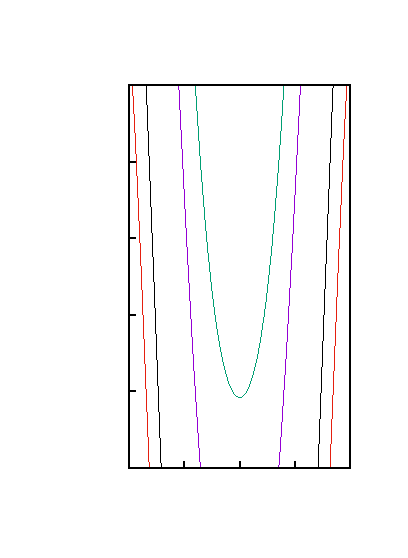
\includegraphics[width={180.00bp},height={252.00bp}]{Lborophene_band-revised}}%
    \gplfronttext
  \end{picture}%
\endgroup
\end{latin}}
\resizebox{0.32\textwidth}{!}{% GNUPLOT: LaTeX picture with Postscript
\begin{latin}
\begingroup
  \makeatletter
  \providecommand\color[2][]{%
    \GenericError{(gnuplot) \space\space\space\@spaces}{%
      Package color not loaded in conjunction with
      terminal option `colourtext'%
    }{See the gnuplot documentation for explanation.%
    }{Either use 'blacktext' in gnuplot or load the package
      color.sty in LaTeX.}%
    \renewcommand\color[2][]{}%
  }%
  \providecommand\includegraphics[2][]{%
    \GenericError{(gnuplot) \space\space\space\@spaces}{%
      Package graphicx or graphics not loaded%
    }{See the gnuplot documentation for explanation.%
    }{The gnuplot epslatex terminal needs graphicx.sty or graphics.sty.}%
    \renewcommand\includegraphics[2][]{}%
  }%
  \providecommand\rotatebox[2]{#2}%
  \@ifundefined{ifGPcolor}{%
    \newif\ifGPcolor
    \GPcolorfalse
  }{}%
  \@ifundefined{ifGPblacktext}{%
    \newif\ifGPblacktext
    \GPblacktexttrue
  }{}%
  % define a \g@addto@macro without @ in the name:
  \let\gplgaddtomacro\g@addto@macro
  % define empty templates for all commands taking text:
  \gdef\gplbacktext{}%
  \gdef\gplfronttext{}%
  \makeatother
  \ifGPblacktext
    % no textcolor at all
    \def\colorrgb#1{}%
    \def\colorgray#1{}%
  \else
    % gray or color?
    \ifGPcolor
      \def\colorrgb#1{\color[rgb]{#1}}%
      \def\colorgray#1{\color[gray]{#1}}%
      \expandafter\def\csname LTw\endcsname{\color{white}}%
      \expandafter\def\csname LTb\endcsname{\color{black}}%
      \expandafter\def\csname LTa\endcsname{\color{black}}%
      \expandafter\def\csname LT0\endcsname{\color[rgb]{1,0,0}}%
      \expandafter\def\csname LT1\endcsname{\color[rgb]{0,1,0}}%
      \expandafter\def\csname LT2\endcsname{\color[rgb]{0,0,1}}%
      \expandafter\def\csname LT3\endcsname{\color[rgb]{1,0,1}}%
      \expandafter\def\csname LT4\endcsname{\color[rgb]{0,1,1}}%
      \expandafter\def\csname LT5\endcsname{\color[rgb]{1,1,0}}%
      \expandafter\def\csname LT6\endcsname{\color[rgb]{0,0,0}}%
      \expandafter\def\csname LT7\endcsname{\color[rgb]{1,0.3,0}}%
      \expandafter\def\csname LT8\endcsname{\color[rgb]{0.5,0.5,0.5}}%
    \else
      % gray
      \def\colorrgb#1{\color{black}}%
      \def\colorgray#1{\color[gray]{#1}}%
      \expandafter\def\csname LTw\endcsname{\color{white}}%
      \expandafter\def\csname LTb\endcsname{\color{black}}%
      \expandafter\def\csname LTa\endcsname{\color{black}}%
      \expandafter\def\csname LT0\endcsname{\color{black}}%
      \expandafter\def\csname LT1\endcsname{\color{black}}%
      \expandafter\def\csname LT2\endcsname{\color{black}}%
      \expandafter\def\csname LT3\endcsname{\color{black}}%
      \expandafter\def\csname LT4\endcsname{\color{black}}%
      \expandafter\def\csname LT5\endcsname{\color{black}}%
      \expandafter\def\csname LT6\endcsname{\color{black}}%
      \expandafter\def\csname LT7\endcsname{\color{black}}%
      \expandafter\def\csname LT8\endcsname{\color{black}}%
    \fi
  \fi
    \setlength{\unitlength}{0.0500bp}%
    \ifx\gptboxheight\undefined%
      \newlength{\gptboxheight}%
      \newlength{\gptboxwidth}%
      \newsavebox{\gptboxtext}%
    \fi%
    \setlength{\fboxrule}{0.5pt}%
    \setlength{\fboxsep}{1pt}%
\begin{picture}(3600.00,5040.00)%
    \gplgaddtomacro\gplbacktext{%
      \csname LTb\endcsname%%
      \put(1400,4200){\makebox(0,0)[r]{\strut{}$B$}}%
      \put(946,704){\makebox(0,0)[r]{\strut{}$-0.8$}}%
      \put(946,1439){\makebox(0,0)[r]{\strut{}$-0.7$}}%
      \put(946,2174){\makebox(0,0)[r]{\strut{}$-0.6$}}%
      \put(946,2909){\makebox(0,0)[r]{\strut{}$-0.5$}}%
      \put(946,3644){\makebox(0,0)[r]{\strut{}$-0.4$}}%
      \put(946,4379){\makebox(0,0)[r]{\strut{}$-0.3$}}%
      \put(1078,484){\makebox(0,0){\strut{}$0$}}%
      \put(1609,484){\makebox(0,0){\strut{}$0.5$}}%
      \put(2141,484){\makebox(0,0){\strut{}$1$}}%
      \put(2672,484){\makebox(0,0){\strut{}$1.5$}}%
      \put(3203,484){\makebox(0,0){\strut{}$2$}}%
      \put(1089,2909){\makebox(0,0)[l]{\strut{}$8\uparrow$}}%
      \put(1344,1439){\makebox(0,0)[l]{\strut{}$8\downarrow$}}%
      \put(1482,2909){\makebox(0,0)[l]{\strut{}$9\uparrow$}}%
      \put(1981,2174){\makebox(0,0)[l]{\strut{}$9\downarrow$}}%
    }%
    \gplgaddtomacro\gplfronttext{%
      \csname LTb\endcsname%%
      \put(209,2541){\rotatebox{-270}{\makebox(0,0){\strut{}$E(eV)$}}}%
      \put(2140,154){\makebox(0,0){\strut{}$k_x$}}%
      \csname LTb\endcsname%%
      \put(2140,4709){\makebox(0,0){\strut{}Center}}%
    }%
    \gplbacktext
    \put(0,0){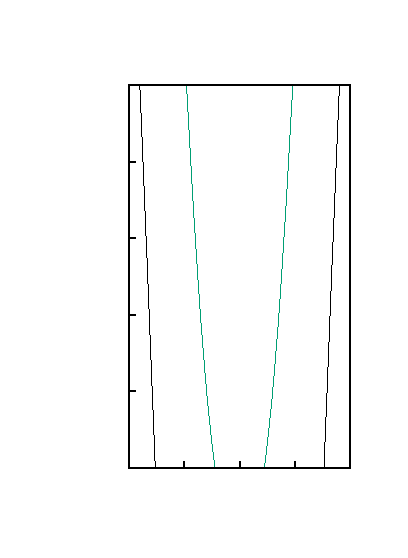
\includegraphics[width={180.00bp},height={252.00bp}]{Cborophene_band-revised}}%
    \gplfronttext
  \end{picture}%
\endgroup
\end{latin}}
\resizebox{0.32\textwidth}{!}{% GNUPLOT: LaTeX picture with Postscript
\begingroup
  \makeatletter
  \providecommand\color[2][]{%
    \GenericError{(gnuplot) \space\space\space\@spaces}{%
      Package color not loaded in conjunction with
      terminal option `colourtext'%
    }{See the gnuplot documentation for explanation.%
    }{Either use 'blacktext' in gnuplot or load the package
      color.sty in LaTeX.}%
    \renewcommand\color[2][]{}%
  }%
  \providecommand\includegraphics[2][]{%
    \GenericError{(gnuplot) \space\space\space\@spaces}{%
      Package graphicx or graphics not loaded%
    }{See the gnuplot documentation for explanation.%
    }{The gnuplot epslatex terminal needs graphicx.sty or graphics.sty.}%
    \renewcommand\includegraphics[2][]{}%
  }%
  \providecommand\rotatebox[2]{#2}%
  \@ifundefined{ifGPcolor}{%
    \newif\ifGPcolor
    \GPcolorfalse
  }{}%
  \@ifundefined{ifGPblacktext}{%
    \newif\ifGPblacktext
    \GPblacktexttrue
  }{}%
  % define a \g@addto@macro without @ in the name:
  \let\gplgaddtomacro\g@addto@macro
  % define empty templates for all commands taking text:
  \gdef\gplbacktext{}%
  \gdef\gplfronttext{}%
  \makeatother
  \ifGPblacktext
    % no textcolor at all
    \def\colorrgb#1{}%
    \def\colorgray#1{}%
  \else
    % gray or color?
    \ifGPcolor
      \def\colorrgb#1{\color[rgb]{#1}}%
      \def\colorgray#1{\color[gray]{#1}}%
      \expandafter\def\csname LTw\endcsname{\color{white}}%
      \expandafter\def\csname LTb\endcsname{\color{black}}%
      \expandafter\def\csname LTa\endcsname{\color{black}}%
      \expandafter\def\csname LT0\endcsname{\color[rgb]{1,0,0}}%
      \expandafter\def\csname LT1\endcsname{\color[rgb]{0,1,0}}%
      \expandafter\def\csname LT2\endcsname{\color[rgb]{0,0,1}}%
      \expandafter\def\csname LT3\endcsname{\color[rgb]{1,0,1}}%
      \expandafter\def\csname LT4\endcsname{\color[rgb]{0,1,1}}%
      \expandafter\def\csname LT5\endcsname{\color[rgb]{1,1,0}}%
      \expandafter\def\csname LT6\endcsname{\color[rgb]{0,0,0}}%
      \expandafter\def\csname LT7\endcsname{\color[rgb]{1,0.3,0}}%
      \expandafter\def\csname LT8\endcsname{\color[rgb]{0.5,0.5,0.5}}%
    \else
      % gray
      \def\colorrgb#1{\color{black}}%
      \def\colorgray#1{\color[gray]{#1}}%
      \expandafter\def\csname LTw\endcsname{\color{white}}%
      \expandafter\def\csname LTb\endcsname{\color{black}}%
      \expandafter\def\csname LTa\endcsname{\color{black}}%
      \expandafter\def\csname LT0\endcsname{\color{black}}%
      \expandafter\def\csname LT1\endcsname{\color{black}}%
      \expandafter\def\csname LT2\endcsname{\color{black}}%
      \expandafter\def\csname LT3\endcsname{\color{black}}%
      \expandafter\def\csname LT4\endcsname{\color{black}}%
      \expandafter\def\csname LT5\endcsname{\color{black}}%
      \expandafter\def\csname LT6\endcsname{\color{black}}%
      \expandafter\def\csname LT7\endcsname{\color{black}}%
      \expandafter\def\csname LT8\endcsname{\color{black}}%
    \fi
  \fi
    \setlength{\unitlength}{0.0500bp}%
    \ifx\gptboxheight\undefined%
      \newlength{\gptboxheight}%
      \newlength{\gptboxwidth}%
      \newsavebox{\gptboxtext}%
    \fi%
    \setlength{\fboxrule}{0.5pt}%
    \setlength{\fboxsep}{1pt}%
\begin{picture}(3600.00,5040.00)%
    \gplgaddtomacro\gplbacktext{%
      \csname LTb\endcsname%%
      \put(1450,4200){\makebox(0,0)[r]{\strut{}$C$}}%
      \put(946,704){\makebox(0,0)[r]{\strut{}$-0.8$}}%
      \put(946,1439){\makebox(0,0)[r]{\strut{}$-0.7$}}%
      \put(946,2174){\makebox(0,0)[r]{\strut{}$-0.6$}}%
      \put(946,2909){\makebox(0,0)[r]{\strut{}$-0.5$}}%
      \put(946,3644){\makebox(0,0)[r]{\strut{}$-0.4$}}%
      \put(946,4379){\makebox(0,0)[r]{\strut{}$-0.3$}}%
      \put(1078,484){\makebox(0,0){\strut{}$0$}}%
      \put(1609,484){\makebox(0,0){\strut{}$0.5$}}%
      \put(2141,484){\makebox(0,0){\strut{}$1$}}%
      \put(2672,484){\makebox(0,0){\strut{}$1.5$}}%
      \put(3203,484){\makebox(0,0){\strut{}$2$}}%
      \put(1089,2909){\makebox(0,0)[l]{\strut{}$8\uparrow$}}%
      \put(1344,1439){\makebox(0,0)[l]{\strut{}$8\downarrow$}}%
      \put(1482,2909){\makebox(0,0)[l]{\strut{}$9\uparrow$}}%
      \put(1981,2174){\makebox(0,0)[l]{\strut{}$9\downarrow$}}%
    }%
    \gplgaddtomacro\gplfronttext{%
      \csname LTb\endcsname%%
      \put(209,2541){\rotatebox{-270}{\makebox(0,0){\strut{}$E(eV)$}}}%
      \put(2140,154){\makebox(0,0){\strut{}$k_x$}}%
      \csname LTb\endcsname%%
      \put(2140,4709){\makebox(0,0){\strut{}Right}}%
    }%
    \gplbacktext
    \put(0,0){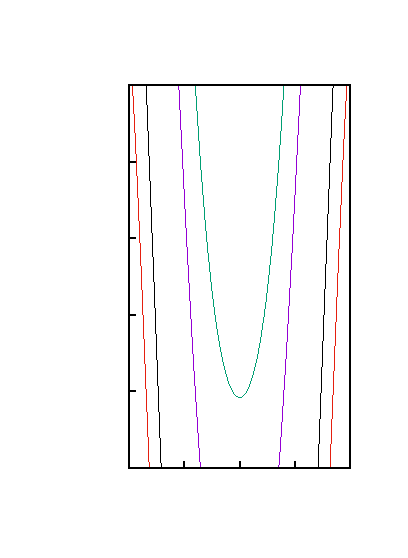
\includegraphics[width={180.00bp},height={252.00bp}]{Rborophene_band-revised}}%
    \gplfronttext
  \end{picture}%
\endgroup
}
\resizebox{0.45\textwidth}{!}{% GNUPLOT: LaTeX picture with Postscript
\begin{latin}
\begingroup
  % Encoding inside the plot.  In the header of your document, this encoding
  % should to defined, e.g., by using
  % \usepackage[cp1252,<other encodings>]{inputenc}
  % \inputencoding{cp1252}%
  \makeatletter
  \providecommand\color[2][]{%
    \GenericError{(gnuplot) \space\space\space\@spaces}{%
      Package color not loaded in conjunction with
      terminal option `colourtext'%
    }{See the gnuplot documentation for explanation.%
    }{Either use 'blacktext' in gnuplot or load the package
      color.sty in LaTeX.}%
    \renewcommand\color[2][]{}%
  }%
  \providecommand\includegraphics[2][]{%
    \GenericError{(gnuplot) \space\space\space\@spaces}{%
      Package graphicx or graphics not loaded%
    }{See the gnuplot documentation for explanation.%
    }{The gnuplot epslatex terminal needs graphicx.sty or graphics.sty.}%
    \renewcommand\includegraphics[2][]{}%
  }%
  \providecommand\rotatebox[2]{#2}%
  \@ifundefined{ifGPcolor}{%
    \newif\ifGPcolor
    \GPcolorfalse
  }{}%
  \@ifundefined{ifGPblacktext}{%
    \newif\ifGPblacktext
    \GPblacktexttrue
  }{}%
  % define a \g@addto@macro without @ in the name:
  \let\gplgaddtomacro\g@addto@macro
  % define empty templates for all commands taking text:
  \gdef\gplbacktext{}%
  \gdef\gplfronttext{}%
  \makeatother
  \ifGPblacktext
    % no textcolor at all
    \def\colorrgb#1{}%
    \def\colorgray#1{}%
  \else
    % gray or color?
    \ifGPcolor
      \def\colorrgb#1{\color[rgb]{#1}}%
      \def\colorgray#1{\color[gray]{#1}}%
      \expandafter\def\csname LTw\endcsname{\color{white}}%
      \expandafter\def\csname LTb\endcsname{\color{black}}%
      \expandafter\def\csname LTa\endcsname{\color{black}}%
      \expandafter\def\csname LT0\endcsname{\color[rgb]{1,0,0}}%
      \expandafter\def\csname LT1\endcsname{\color[rgb]{0,1,0}}%
      \expandafter\def\csname LT2\endcsname{\color[rgb]{0,0,1}}%
      \expandafter\def\csname LT3\endcsname{\color[rgb]{1,0,1}}%
      \expandafter\def\csname LT4\endcsname{\color[rgb]{0,1,1}}%
      \expandafter\def\csname LT5\endcsname{\color[rgb]{1,1,0}}%
      \expandafter\def\csname LT6\endcsname{\color[rgb]{0,0,0}}%
      \expandafter\def\csname LT7\endcsname{\color[rgb]{1,0.3,0}}%
      \expandafter\def\csname LT8\endcsname{\color[rgb]{0.5,0.5,0.5}}%
    \else
      % gray
      \def\colorrgb#1{\color{black}}%
      \def\colorgray#1{\color[gray]{#1}}%
      \expandafter\def\csname LTw\endcsname{\color{white}}%
      \expandafter\def\csname LTb\endcsname{\color{black}}%
      \expandafter\def\csname LTa\endcsname{\color{black}}%
      \expandafter\def\csname LT0\endcsname{\color{black}}%
      \expandafter\def\csname LT1\endcsname{\color{black}}%
      \expandafter\def\csname LT2\endcsname{\color{black}}%
      \expandafter\def\csname LT3\endcsname{\color{black}}%
      \expandafter\def\csname LT4\endcsname{\color{black}}%
      \expandafter\def\csname LT5\endcsname{\color{black}}%
      \expandafter\def\csname LT6\endcsname{\color{black}}%
      \expandafter\def\csname LT7\endcsname{\color{black}}%
      \expandafter\def\csname LT8\endcsname{\color{black}}%
    \fi
  \fi
    \setlength{\unitlength}{0.0500bp}%
    \ifx\gptboxheight\undefined%
      \newlength{\gptboxheight}%
      \newlength{\gptboxwidth}%
      \newsavebox{\gptboxtext}%
    \fi%
    \setlength{\fboxrule}{0.5pt}%
    \setlength{\fboxsep}{1pt}%
\begin{picture}(7200.00,5040.00)%
    \gplgaddtomacro\gplbacktext{%
      \csname LTb\endcsname%%
      \put(1200,4200){\makebox(0,0)[r]{\strut{}$D$}}%
      \put(814,704){\makebox(0,0)[r]{\strut{}$1$}}%
      \put(814,1229){\makebox(0,0)[r]{\strut{}$1.5$}}%
      \put(814,1754){\makebox(0,0)[r]{\strut{}$2$}}%
      \put(814,2279){\makebox(0,0)[r]{\strut{}$2.5$}}%
      \put(814,2804){\makebox(0,0)[r]{\strut{}$3$}}%
      \put(814,3329){\makebox(0,0)[r]{\strut{}$3.5$}}%
      \put(814,3854){\makebox(0,0)[r]{\strut{}$4$}}%
      \put(814,4379){\makebox(0,0)[r]{\strut{}$4.5$}}%
      \put(946,484){\makebox(0,0){\strut{}$-1$}}%
      \put(2117,484){\makebox(0,0){\strut{}$-0.8$}}%
      \put(3289,484){\makebox(0,0){\strut{}$-0.6$}}%
      \put(4460,484){\makebox(0,0){\strut{}$-0.4$}}%
      \put(5632,484){\makebox(0,0){\strut{}$-0.2$}}%
      \put(6803,484){\makebox(0,0){\strut{}$0$}}%
    }%
    \gplgaddtomacro\gplfronttext{%
      \csname LTb\endcsname%%
      \put(209,2541){\rotatebox{-270}{\makebox(0,0){\strut{}$G(e^2/h)$}}}%
      \put(3874,154){\makebox(0,0){\strut{}$E(eV)$}}%
      \csname LTb\endcsname%%
      \put(2522,4206){\makebox(0,0)[r]{\strut{}$M=0$}}%
      \csname LTb\endcsname%%
      \put(2522,3986){\makebox(0,0)[r]{\strut{}$M=0.05$}}%
      \csname LTb\endcsname%%
      \put(4169,4206){\makebox(0,0)[r]{\strut{}$M=0.1$}}%
      \csname LTb\endcsname%%
      \put(4169,3986){\makebox(0,0)[r]{\strut{}$M=0.2$}}%
      \csname LTb\endcsname%%
      \put(5816,4206){\makebox(0,0)[r]{\strut{}$M=0.3$}}%
      \csname LTb\endcsname%%
      \put(3874,4709){\makebox(0,0){\strut{}Parallel}}%
    }%
    \gplbacktext
    \put(0,0){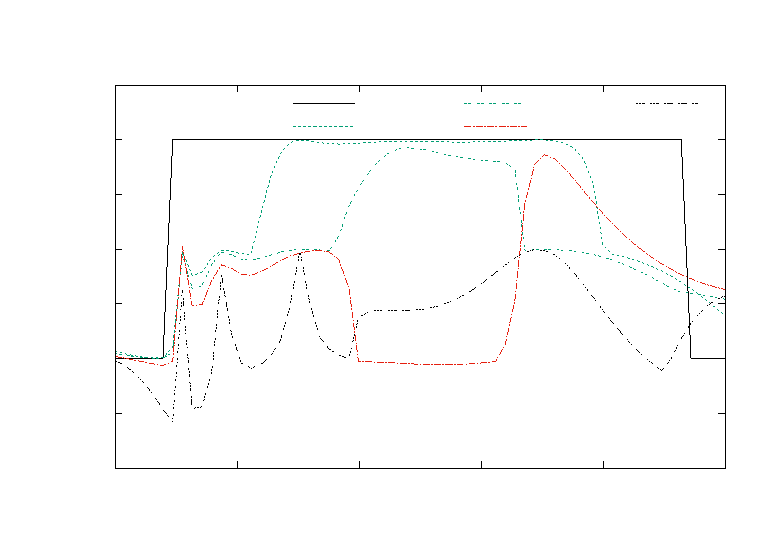
\includegraphics[width={360.00bp},height={252.00bp}]{armchair-parallel-conductance-1to0-revise}}%
    \gplfronttext
  \end{picture}%
\endgroup
\end{latin}}
\resizebox{0.45\textwidth}{!}{\input{./figures/armchair-Antiparallel-conductance-1to0-revise.tex}}
\caption{A, B, C) در لید سمت چپ، برای تعداد زوج اتم در سوپرسل، برای مثال، باند شماره 8 (یا 9) با عدد اتم $8(9)$ مطابقت دارد که به دو زیر باند spin up $ تقسیم می شود. (8^\uparrow)$ و وقتی تعامل چرخش گنجانده شده است، $(8\downarrow)$ را به پایین بچرخانید: الف) در پیکربندی P، زیر باندهای $(8\uparrow)$ در هر دو لید چپ و راست در بالای زیر باندهای $(8\downarrow)$ با برابری یکسان است و بنابراین انتقال الکترون مجاز است. ب) در پیکربندی‌های AP، $(8\uparrow)$، در یک لید، بالاتر از زیر باند $(8\downarrow)$ در همان لید قرار دارد، در حالی که در لید دیگر، $(8\uparrow) $ در زیر باند $(8\downarrow)$ پایین تر با برابری مخالف قرار دارد و بنابراین انتقال الکترون مجاز نیست. D، E) نمودار رسانایی در محدوده انرژی یکسان ساختار نواری برای پیکربندی‌های P و AP.}
\label{fig:bandconductance}
\end{figure*}

\begin{figure*}
\centering
\resizebox{0.45\textwidth}{!}{% GNUPLOT: LaTeX picture with Postscript
\begingroup
  % Encoding inside the plot.  In the header of your document, this encoding
  % should to defined, e.g., by using
  % \usepackage[cp1252,<other encodings>]{inputenc}
  % \inputencoding{cp1252}%
  \makeatletter
  \providecommand\color[2][]{%
    \GenericError{(gnuplot) \space\space\space\@spaces}{%
      Package color not loaded in conjunction with
      terminal option `colourtext'%
    }{See the gnuplot documentation for explanation.%
    }{Either use 'blacktext' in gnuplot or load the package
      color.sty in LaTeX.}%
    \renewcommand\color[2][]{}%
  }%
  \providecommand\includegraphics[2][]{%
    \GenericError{(gnuplot) \space\space\space\@spaces}{%
      Package graphicx or graphics not loaded%
    }{See the gnuplot documentation for explanation.%
    }{The gnuplot epslatex terminal needs graphicx.sty or graphics.sty.}%
    \renewcommand\includegraphics[2][]{}%
  }%
  \providecommand\rotatebox[2]{#2}%
  \@ifundefined{ifGPcolor}{%
    \newif\ifGPcolor
    \GPcolorfalse
  }{}%
  \@ifundefined{ifGPblacktext}{%
    \newif\ifGPblacktext
    \GPblacktexttrue
  }{}%
  % define a \g@addto@macro without @ in the name:
  \let\gplgaddtomacro\g@addto@macro
  % define empty templates for all commands taking text:
  \gdef\gplbacktext{}%
  \gdef\gplfronttext{}%
  \makeatother
  \ifGPblacktext
    % no textcolor at all
    \def\colorrgb#1{}%
    \def\colorgray#1{}%
  \else
    % gray or color?
    \ifGPcolor
      \def\colorrgb#1{\color[rgb]{#1}}%
      \def\colorgray#1{\color[gray]{#1}}%
      \expandafter\def\csname LTw\endcsname{\color{white}}%
      \expandafter\def\csname LTb\endcsname{\color{black}}%
      \expandafter\def\csname LTa\endcsname{\color{black}}%
      \expandafter\def\csname LT0\endcsname{\color[rgb]{1,0,0}}%
      \expandafter\def\csname LT1\endcsname{\color[rgb]{0,1,0}}%
      \expandafter\def\csname LT2\endcsname{\color[rgb]{0,0,1}}%
      \expandafter\def\csname LT3\endcsname{\color[rgb]{1,0,1}}%
      \expandafter\def\csname LT4\endcsname{\color[rgb]{0,1,1}}%
      \expandafter\def\csname LT5\endcsname{\color[rgb]{1,1,0}}%
      \expandafter\def\csname LT6\endcsname{\color[rgb]{0,0,0}}%
      \expandafter\def\csname LT7\endcsname{\color[rgb]{1,0.3,0}}%
      \expandafter\def\csname LT8\endcsname{\color[rgb]{0.5,0.5,0.5}}%
    \else
      % gray
      \def\colorrgb#1{\color{black}}%
      \def\colorgray#1{\color[gray]{#1}}%
      \expandafter\def\csname LTw\endcsname{\color{white}}%
      \expandafter\def\csname LTb\endcsname{\color{black}}%
      \expandafter\def\csname LTa\endcsname{\color{black}}%
      \expandafter\def\csname LT0\endcsname{\color{black}}%
      \expandafter\def\csname LT1\endcsname{\color{black}}%
      \expandafter\def\csname LT2\endcsname{\color{black}}%
      \expandafter\def\csname LT3\endcsname{\color{black}}%
      \expandafter\def\csname LT4\endcsname{\color{black}}%
      \expandafter\def\csname LT5\endcsname{\color{black}}%
      \expandafter\def\csname LT6\endcsname{\color{black}}%
      \expandafter\def\csname LT7\endcsname{\color{black}}%
      \expandafter\def\csname LT8\endcsname{\color{black}}%
    \fi
  \fi
    \setlength{\unitlength}{0.0500bp}%
    \ifx\gptboxheight\undefined%
      \newlength{\gptboxheight}%
      \newlength{\gptboxwidth}%
      \newsavebox{\gptboxtext}%
    \fi%
    \setlength{\fboxrule}{0.5pt}%
    \setlength{\fboxsep}{1pt}%
\begin{picture}(7200.00,5040.00)%
    \gplgaddtomacro\gplbacktext{%
      \csname LTb\endcsname%%
      \put(1400,4600){\makebox(0,0)[r]{\strut{}$A$}}%
      \put(814,1077){\makebox(0,0)[r]{\strut{}$0$}}%
      \put(814,1635){\makebox(0,0)[r]{\strut{}$0.2$}}%
      \put(814,2193){\makebox(0,0)[r]{\strut{}$0.4$}}%
      \put(814,2751){\makebox(0,0)[r]{\strut{}$0.6$}}%
      \put(814,3309){\makebox(0,0)[r]{\strut{}$0.8$}}%
      \put(814,3867){\makebox(0,0)[r]{\strut{}$1$}}%
      \put(946,857){\makebox(0,0){\strut{}$-4$}}%
      \put(1678,857){\makebox(0,0){\strut{}$-3$}}%
      \put(2410,857){\makebox(0,0){\strut{}$-2$}}%
      \put(3142,857){\makebox(0,0){\strut{}$-1$}}%
      \put(3875,857){\makebox(0,0){\strut{}$0$}}%
      \put(4607,857){\makebox(0,0){\strut{}$1$}}%
      \put(5339,857){\makebox(0,0){\strut{}$2$}}%
      \put(6071,857){\makebox(0,0){\strut{}$3$}}%
      \put(6803,857){\makebox(0,0){\strut{}$4$}}%
    }%
    \gplgaddtomacro\gplfronttext{%
      \csname LTb\endcsname%%
      \put(209,2541){\rotatebox{-270}{\makebox(0,0){\strut{}MR}}}%
      \put(3874,527){\makebox(0,0){\strut{}$E(eV)$}}%
      \csname LTb\endcsname%%
      \put(2654,4867){\makebox(0,0)[r]{\strut{}$M=0$}}%
      \csname LTb\endcsname%%
      \put(2654,4647){\makebox(0,0)[r]{\strut{}$M=0.05$}}%
      \csname LTb\endcsname%%
      \put(4301,4867){\makebox(0,0)[r]{\strut{}$M=0.1$}}%
      \csname LTb\endcsname%%
      \put(4301,4647){\makebox(0,0)[r]{\strut{}$M=0.2$}}%
      \csname LTb\endcsname%%
      \put(5948,4867){\makebox(0,0)[r]{\strut{}$M=0.3$}}%
    }%
    \gplbacktext
    \put(0,0){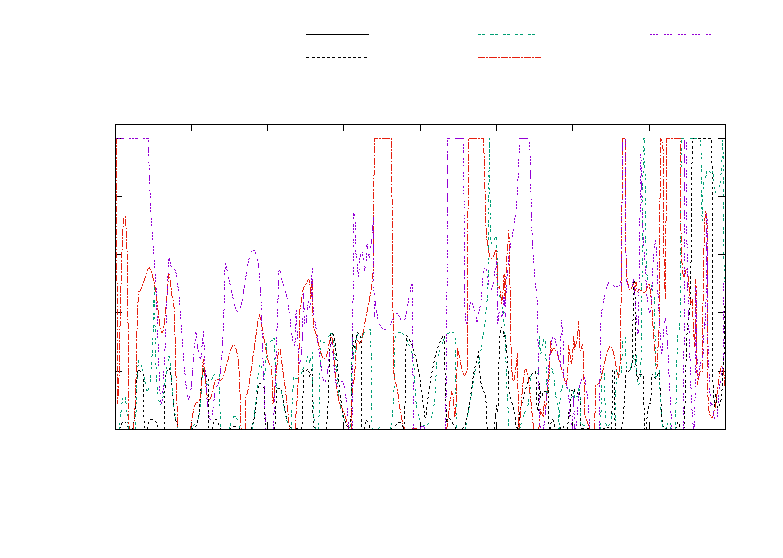
\includegraphics[width={360.00bp},height={252.00bp}]{MR-revise}}%
    \gplfronttext
  \end{picture}%
\endgroup
}
\resizebox{0.45\textwidth}{!}{% GNUPLOT: LaTeX picture with Postscript
\begingroup
  % Encoding inside the plot.  In the header of your document, this encoding
  % should to defined, e.g., by using
  % \usepackage[cp1252,<other encodings>]{inputenc}
  % \inputencoding{cp1252}%s
  \makeatletter
  \providecommand\color[2][]{%
    \GenericError{(gnuplot) \space\space\space\@spaces}{%
      Package color not loaded in conjunction with
      terminal option `colourtext'%
    }{See the gnuplot documentation for explanation.%
    }{Either use 'blacktext' in gnuplot or load the package
      color.sty in LaTeX.}%
    \renewcommand\color[2][]{}%
  }%
  \providecommand\includegraphics[2][]{%
    \GenericError{(gnuplot) \space\space\space\@spaces}{%
      Package graphicx or graphics not loaded%
    }{See the gnuplot documentation for explanation.%
    }{The gnuplot epslatex terminal needs graphicx.sty or graphics.sty.}%
    \renewcommand\includegraphics[2][]{}%
  }%
  \providecommand\rotatebox[2]{#2}%
  \@ifundefined{ifGPcolor}{%
    \newif\ifGPcolor
    \GPcolorfalse
  }{}%
  \@ifundefined{ifGPblacktext}{%
    \newif\ifGPblacktext
    \GPblacktexttrue
  }{}%
  % define a \g@addto@macro without @ in the name:
  \let\gplgaddtomacro\g@addto@macro
  % define empty templates for all commands taking text:
  \gdef\gplbacktext{}%
  \gdef\gplfronttext{}%
  \makeatother
  \ifGPblacktext
    % no textcolor at all
    \def\colorrgb#1{}%
    \def\colorgray#1{}%
  \else
    % gray or color?
    \ifGPcolor
      \def\colorrgb#1{\color[rgb]{#1}}%
      \def\colorgray#1{\color[gray]{#1}}%
      \expandafter\def\csname LTw\endcsname{\color{white}}%
      \expandafter\def\csname LTb\endcsname{\color{black}}%
      \expandafter\def\csname LTa\endcsname{\color{black}}%
      \expandafter\def\csname LT0\endcsname{\color[rgb]{1,0,0}}%
      \expandafter\def\csname LT1\endcsname{\color[rgb]{0,1,0}}%
      \expandafter\def\csname LT2\endcsname{\color[rgb]{0,0,1}}%
      \expandafter\def\csname LT3\endcsname{\color[rgb]{1,0,1}}%
      \expandafter\def\csname LT4\endcsname{\color[rgb]{0,1,1}}%
      \expandafter\def\csname LT5\endcsname{\color[rgb]{1,1,0}}%
      \expandafter\def\csname LT6\endcsname{\color[rgb]{0,0,0}}%
      \expandafter\def\csname LT7\endcsname{\color[rgb]{1,0.3,0}}%
      \expandafter\def\csname LT8\endcsname{\color[rgb]{0.5,0.5,0.5}}%
    \else
      % gray
      \def\colorrgb#1{\color{black}}%
      \def\colorgray#1{\color[gray]{#1}}%
      \expandafter\def\csname LTw\endcsname{\color{white}}%
      \expandafter\def\csname LTb\endcsname{\color{black}}%
      \expandafter\def\csname LTa\endcsname{\color{black}}%
      \expandafter\def\csname LT0\endcsname{\color{black}}%
      \expandafter\def\csname LT1\endcsname{\color{black}}%
      \expandafter\def\csname LT2\endcsname{\color{black}}%
      \expandafter\def\csname LT3\endcsname{\color{black}}%
      \expandafter\def\csname LT4\endcsname{\color{black}}%
      \expandafter\def\csname LT5\endcsname{\color{black}}%
      \expandafter\def\csname LT6\endcsname{\color{black}}%
      \expandafter\def\csname LT7\endcsname{\color{black}}%
      \expandafter\def\csname LT8\endcsname{\color{black}}%
    \fi
  \fi
    \setlength{\unitlength}{0.0500bp}%
    \ifx\gptboxheight\undefined%
      \newlength{\gptboxheight}%
      \newlength{\gptboxwidth}%
      \newsavebox{\gptboxtext}%
    \fi%
    \setlength{\fboxrule}{0.5pt}%
    \setlength{\fboxsep}{1pt}%
\begin{picture}(7200.00,5040.00)%
    \gplgaddtomacro\gplbacktext{%
      \csname LTb\endcsname%%
      \put(1400,4600){\makebox(0,0)[r]{\strut{}$B$}}%
      \put(814,1077){\makebox(0,0)[r]{\strut{}$0$}}%
      \put(814,1635){\makebox(0,0)[r]{\strut{}$0.2$}}%
      \put(814,2193){\makebox(0,0)[r]{\strut{}$0.4$}}%
      \put(814,2751){\makebox(0,0)[r]{\strut{}$0.6$}}%
      \put(814,3309){\makebox(0,0)[r]{\strut{}$0.8$}}%
      \put(814,3867){\makebox(0,0)[r]{\strut{}$1$}}%
      \put(946,857){\makebox(0,0){\strut{}$-4$}}%
      \put(1678,857){\makebox(0,0){\strut{}$-3$}}%
      \put(2410,857){\makebox(0,0){\strut{}$-2$}}%
      \put(3142,857){\makebox(0,0){\strut{}$-1$}}%
      \put(3875,857){\makebox(0,0){\strut{}$0$}}%
      \put(4607,857){\makebox(0,0){\strut{}$1$}}%
      \put(5339,857){\makebox(0,0){\strut{}$2$}}%
      \put(6071,857){\makebox(0,0){\strut{}$3$}}%
      \put(6803,857){\makebox(0,0){\strut{}$4$}}%
    }%
    \gplgaddtomacro\gplfronttext{%
      \csname LTb\endcsname%%
      \put(209,2541){\rotatebox{-270}{\makebox(0,0){\strut{}MR}}}%
      \put(3874,527){\makebox(0,0){\strut{}$E(eV)$}}%
      \csname LTb\endcsname%%
      \put(2654,4867){\makebox(0,0)[r]{\strut{}$M=0$}}%
      \csname LTb\endcsname%%
      \put(2654,4647){\makebox(0,0)[r]{\strut{}$M=0.05$}}%
      \csname LTb\endcsname%%
      \put(4301,4867){\makebox(0,0)[r]{\strut{}$M=0.1$}}%
      \csname LTb\endcsname%%
      \put(4301,4647){\makebox(0,0)[r]{\strut{}$M=0.2$}}%
      \csname LTb\endcsname%%
      \put(5948,4867){\makebox(0,0)[r]{\strut{}$M=0.3$}}%
    }%
    \gplbacktext
    \put(0,0){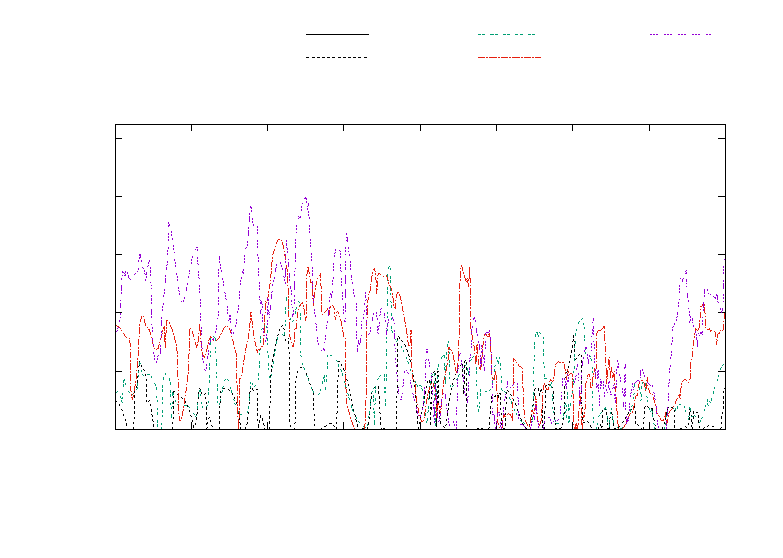
\includegraphics[width={360.00bp},height={252.00bp}]{MR_zig-revise}}%
    \gplfronttext
  \end{picture}%
\endgroup
}
\caption{مقاومت مغناطیس (MR) $\beta_{12}$-بوروفن در صندلی راحتی و لبه‌های زیگزاگی.}
\label{fig:MR}
\end{figure*}

\begin{figure*}[ht]
    \centering
    \resizebox{0.45\textwidth}{!}{% GNUPLOT: LaTeX picture with Postscript
\begin{latin}
\begingroup
  % Encoding inside the plot.  In the header of your document, this encoding
  % should to defined, e.g., by using
  % \usepackage[cp1252,<other encodings>]{inputenc}
  % \inputencoding{cp1252}%
  \makeatletter
  \providecommand\color[2][]{%
    \GenericError{(gnuplot) \space\space\space\@spaces}{%
      Package color not loaded in conjunction with
      terminal option `colourtext'%
    }{See the gnuplot documentation for explanation.%
    }{Either use 'blacktext' in gnuplot or load the package
      color.sty in LaTeX.}%
    \renewcommand\color[2][]{}%
  }%
  \providecommand\includegraphics[2][]{%
    \GenericError{(gnuplot) \space\space\space\@spaces}{%
      Package graphicx or graphics not loaded%
    }{See the gnuplot documentation for explanation.%
    }{The gnuplot epslatex terminal needs graphicx.sty or graphics.sty.}%
    \renewcommand\includegraphics[2][]{}%
  }%
  \providecommand\rotatebox[2]{#2}%
  \@ifundefined{ifGPcolor}{%
    \newif\ifGPcolor
    \GPcolorfalse
  }{}%
  \@ifundefined{ifGPblacktext}{%
    \newif\ifGPblacktext
    \GPblacktexttrue
  }{}%
  % define a \g@addto@macro without @ in the name:
  \let\gplgaddtomacro\g@addto@macro
  % define empty templates for all commands taking text:
  \gdef\gplbacktext{}%
  \gdef\gplfronttext{}%
  \makeatother
  \ifGPblacktext
    % no textcolor at all
    \def\colorrgb#1{}%
    \def\colorgray#1{}%
  \else
    % gray or color?
    \ifGPcolor
      \def\colorrgb#1{\color[rgb]{#1}}%
      \def\colorgray#1{\color[gray]{#1}}%
      \expandafter\def\csname LTw\endcsname{\color{white}}%
      \expandafter\def\csname LTb\endcsname{\color{black}}%
      \expandafter\def\csname LTa\endcsname{\color{black}}%
      \expandafter\def\csname LT0\endcsname{\color[rgb]{1,0,0}}%
      \expandafter\def\csname LT1\endcsname{\color[rgb]{0,1,0}}%
      \expandafter\def\csname LT2\endcsname{\color[rgb]{0,0,1}}%
      \expandafter\def\csname LT3\endcsname{\color[rgb]{1,0,1}}%
      \expandafter\def\csname LT4\endcsname{\color[rgb]{0,1,1}}%
      \expandafter\def\csname LT5\endcsname{\color[rgb]{1,1,0}}%
      \expandafter\def\csname LT6\endcsname{\color[rgb]{0,0,0}}%
      \expandafter\def\csname LT7\endcsname{\color[rgb]{1,0.3,0}}%
      \expandafter\def\csname LT8\endcsname{\color[rgb]{0.5,0.5,0.5}}%
    \else
      % gray
      \def\colorrgb#1{\color{black}}%
      \def\colorgray#1{\color[gray]{#1}}%
      \expandafter\def\csname LTw\endcsname{\color{white}}%
      \expandafter\def\csname LTb\endcsname{\color{black}}%
      \expandafter\def\csname LTa\endcsname{\color{black}}%
      \expandafter\def\csname LT0\endcsname{\color{black}}%
      \expandafter\def\csname LT1\endcsname{\color{black}}%
      \expandafter\def\csname LT2\endcsname{\color{black}}%
      \expandafter\def\csname LT3\endcsname{\color{black}}%
      \expandafter\def\csname LT4\endcsname{\color{black}}%
      \expandafter\def\csname LT5\endcsname{\color{black}}%
      \expandafter\def\csname LT6\endcsname{\color{black}}%
      \expandafter\def\csname LT7\endcsname{\color{black}}%
      \expandafter\def\csname LT8\endcsname{\color{black}}%
    \fi
  \fi
    \setlength{\unitlength}{0.0500bp}%
    \ifx\gptboxheight\undefined%
      \newlength{\gptboxheight}%
      \newlength{\gptboxwidth}%
      \newsavebox{\gptboxtext}%
    \fi%
    \setlength{\fboxrule}{0.5pt}%
    \setlength{\fboxsep}{1pt}%
\begin{picture}(7200.00,5040.00)%
    \gplgaddtomacro\gplbacktext{%
      \csname LTb\endcsname%%
      \put(1300,4200){\makebox(0,0)[r]{\strut{}$A$}}%
      \put(946,704){\makebox(0,0)[r]{\strut{}$-0.3$}}%
      \put(946,1323){\makebox(0,0)[r]{\strut{}$-0.2$}}%
      \put(946,1942){\makebox(0,0)[r]{\strut{}$-0.1$}}%
      \put(946,2562){\makebox(0,0)[r]{\strut{}$0$}}%
      \put(946,3181){\makebox(0,0)[r]{\strut{}$0.1$}}%
      \put(946,3800){\makebox(0,0)[r]{\strut{}$0.2$}}%
      \put(946,4419){\makebox(0,0)[r]{\strut{}$0.3$}}%
      \put(1078,484){\makebox(0,0){\strut{}$0$}}%
      \put(2509,484){\makebox(0,0){\strut{}$0.5$}}%
      \put(3941,484){\makebox(0,0){\strut{}$1$}}%
      \put(5372,484){\makebox(0,0){\strut{}$1.5$}}%
      \put(6803,484){\makebox(0,0){\strut{}$2$}}%
    }%
    \gplgaddtomacro\gplfronttext{%
      \csname LTb\endcsname%%
      \put(209,2561){\rotatebox{-270}{\makebox(0,0){\strut{}$\tau/V$}}}%
      \put(3940,154){\makebox(0,0){\strut{}$\theta$}}%
      \csname LTb\endcsname%%
      \put(5816,4246){\makebox(0,0)[r]{\strut{}$M=0.05$}}%
      \csname LTb\endcsname%%
      \put(5816,4026){\makebox(0,0)[r]{\strut{}$M=0.10$}}%
      \csname LTb\endcsname%%
      \put(5816,3806){\makebox(0,0)[r]{\strut{}$M=0.20$}}%
      \csname LTb\endcsname%%
      \put(5816,3586){\makebox(0,0)[r]{\strut{}$M=0.30$}}%
      \csname LTb\endcsname%%
      \put(3940,4709){\makebox(0,0){\strut{}Spin Torque 2D}}%
    }%
    \gplbacktext
    \put(0,0){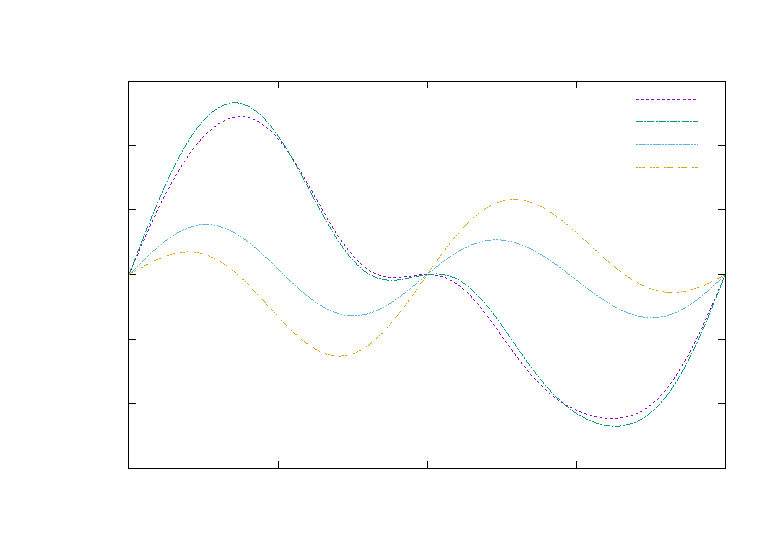
\includegraphics[width={360.00bp},height={252.00bp}]{stt}}%
    \gplfronttext
  \end{picture}%
\endgroup
\end{latin}}
    \resizebox{0.45\textwidth}{!}{% GNUPLOT: LaTeX picture with Postscript
\begingroup
  % Encoding inside the plot.  In the header of your document, this encoding
  % should to defined, e.g., by using
  % \usepackage[cp1252,<other encodings>]{inputenc}
  % \inputencoding{cp1252}%
  \makeatletter
  \providecommand\color[2][]{%
    \GenericError{(gnuplot) \space\space\space\@spaces}{%
      Package color not loaded in conjunction with
      terminal option `colourtext'%
    }{See the gnuplot documentation for explanation.%
    }{Either use 'blacktext' in gnuplot or load the package
      color.sty in LaTeX.}%
    \renewcommand\color[2][]{}%
  }%
  \providecommand\includegraphics[2][]{%
    \GenericError{(gnuplot) \space\space\space\@spaces}{%
      Package graphicx or graphics not loaded%
    }{See the gnuplot documentation for explanation.%
    }{The gnuplot epslatex terminal needs graphicx.sty or graphics.sty.}%
    \renewcommand\includegraphics[2][]{}%
  }%
  \providecommand\rotatebox[2]{#2}%
  \@ifundefined{ifGPcolor}{%
    \newif\ifGPcolor
    \GPcolorfalse
  }{}%
  \@ifundefined{ifGPblacktext}{%
    \newif\ifGPblacktext
    \GPblacktexttrue
  }{}%
  % define a \g@addto@macro without @ in the name:
  \let\gplgaddtomacro\g@addto@macro
  % define empty templates for all commands taking text:
  \gdef\gplbacktext{}%
  \gdef\gplfronttext{}%
  \makeatother
  \ifGPblacktext
    % no textcolor at all
    \def\colorrgb#1{}%
    \def\colorgray#1{}%
  \else
    % gray or color?
    \ifGPcolor
      \def\colorrgb#1{\color[rgb]{#1}}%
      \def\colorgray#1{\color[gray]{#1}}%
      \expandafter\def\csname LTw\endcsname{\color{white}}%
      \expandafter\def\csname LTb\endcsname{\color{black}}%
      \expandafter\def\csname LTa\endcsname{\color{black}}%
      \expandafter\def\csname LT0\endcsname{\color[rgb]{1,0,0}}%
      \expandafter\def\csname LT1\endcsname{\color[rgb]{0,1,0}}%
      \expandafter\def\csname LT2\endcsname{\color[rgb]{0,0,1}}%
      \expandafter\def\csname LT3\endcsname{\color[rgb]{1,0,1}}%
      \expandafter\def\csname LT4\endcsname{\color[rgb]{0,1,1}}%
      \expandafter\def\csname LT5\endcsname{\color[rgb]{1,1,0}}%
      \expandafter\def\csname LT6\endcsname{\color[rgb]{0,0,0}}%
      \expandafter\def\csname LT7\endcsname{\color[rgb]{1,0.3,0}}%
      \expandafter\def\csname LT8\endcsname{\color[rgb]{0.5,0.5,0.5}}%
    \else
      % gray
      \def\colorrgb#1{\color{black}}%
      \def\colorgray#1{\color[gray]{#1}}%
      \expandafter\def\csname LTw\endcsname{\color{white}}%
      \expandafter\def\csname LTb\endcsname{\color{black}}%
      \expandafter\def\csname LTa\endcsname{\color{black}}%
      \expandafter\def\csname LT0\endcsname{\color{black}}%
      \expandafter\def\csname LT1\endcsname{\color{black}}%
      \expandafter\def\csname LT2\endcsname{\color{black}}%
      \expandafter\def\csname LT3\endcsname{\color{black}}%
      \expandafter\def\csname LT4\endcsname{\color{black}}%
      \expandafter\def\csname LT5\endcsname{\color{black}}%
      \expandafter\def\csname LT6\endcsname{\color{black}}%
      \expandafter\def\csname LT7\endcsname{\color{black}}%
      \expandafter\def\csname LT8\endcsname{\color{black}}%
    \fi
  \fi
    \setlength{\unitlength}{0.0500bp}%
    \ifx\gptboxheight\undefined%
      \newlength{\gptboxheight}%
      \newlength{\gptboxwidth}%
      \newsavebox{\gptboxtext}%
    \fi%
    \setlength{\fboxrule}{0.5pt}%
    \setlength{\fboxsep}{1pt}%
\begin{picture}(7200.00,5040.00)%
    \gplgaddtomacro\gplbacktext{%
    }%
    \gplgaddtomacro\gplfronttext{%
      \csname LTb\endcsname%%
      \put(1300,3900){\makebox(0,0)[r]{\strut{}$B$}}%
      \put(936,674){\makebox(0,0){\strut{}$-4$}}%
      \put(1602,674){\makebox(0,0){\strut{}$-3$}}%
      \put(2268,674){\makebox(0,0){\strut{}$-2$}}%
      \put(2934,674){\makebox(0,0){\strut{}$-1$}}%
      \put(3600,674){\makebox(0,0){\strut{}$0$}}%
      \put(4266,674){\makebox(0,0){\strut{}$1$}}%
      \put(4932,674){\makebox(0,0){\strut{}$2$}}%
      \put(5598,674){\makebox(0,0){\strut{}$3$}}%
      \put(6264,674){\makebox(0,0){\strut{}$4$}}%
      \put(3600,344){\makebox(0,0){\strut{}$E(eV)$}}%
      \put(693,917){\makebox(0,0)[r]{\strut{}$-6$}}%
      \put(693,1318){\makebox(0,0)[r]{\strut{}$-4$}}%
      \put(693,1719){\makebox(0,0)[r]{\strut{}$-2$}}%
      \put(693,2120){\makebox(0,0)[r]{\strut{}$0$}}%
      \put(693,2520){\makebox(0,0)[r]{\strut{}$2$}}%
      \put(693,2920){\makebox(0,0)[r]{\strut{}$4$}}%
      \put(693,3321){\makebox(0,0)[r]{\strut{}$6$}}%
      \put(693,3722){\makebox(0,0)[r]{\strut{}$8$}}%
      \put(693,4123){\makebox(0,0)[r]{\strut{}$10$}}%
      \put(363,2520){\rotatebox{-270}{\makebox(0,0){\strut{}$\tau$}}}%
      \put(6795,917){\makebox(0,0)[l]{\strut{}$0$}}%
      \put(6795,1237){\makebox(0,0)[l]{\strut{}$0.2$}}%
      \put(6795,1558){\makebox(0,0)[l]{\strut{}$0.4$}}%
      \put(6795,1878){\makebox(0,0)[l]{\strut{}$0.6$}}%
      \put(6795,2199){\makebox(0,0)[l]{\strut{}$0.8$}}%
      \put(6795,2520){\makebox(0,0)[l]{\strut{}$1$}}%
      \put(6795,2840){\makebox(0,0)[l]{\strut{}$1.2$}}%
      \put(6795,3161){\makebox(0,0)[l]{\strut{}$1.4$}}%
      \put(6795,3481){\makebox(0,0)[l]{\strut{}$1.6$}}%
      \put(6795,3802){\makebox(0,0)[l]{\strut{}$1.8$}}%
      \put(6795,4123){\makebox(0,0)[l]{\strut{}$2$}}%
      \put(7257,2520){\rotatebox{-270}{\makebox(0,0){\strut{}$\theta$}}}%
      \put(3600,4453){\makebox(0,0){\strut{}$M=0.1$}}%
    }%
    \gplbacktext
    \put(0,0){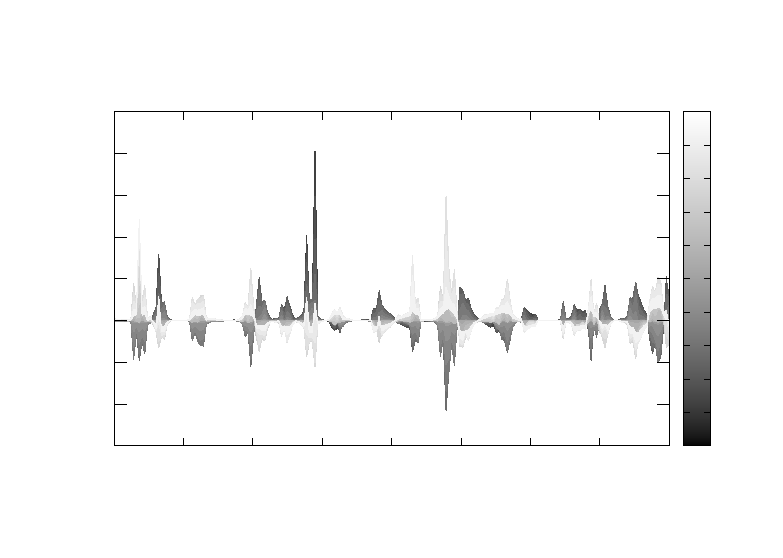
\includegraphics[width={360.00bp},height={252.00bp}]{stt-energy3d-0.1}}%
    \gplfronttext
  \end{picture}%
\endgroup
}
    \resizebox{0.45\textwidth}{!}{% GNUPLOT: LaTeX picture with Postscript
\begingroup
  % Encoding inside the plot.  In the header of your document, this encoding
  % should to defined, e.g., by using
  % \usepackage[cp1252,<other encodings>]{inputenc}
  % \inputencoding{cp1252}%
  \makeatletter
  \providecommand\color[2][]{%
    \GenericError{(gnuplot) \space\space\space\@spaces}{%
      Package color not loaded in conjunction with
      terminal option `colourtext'%
    }{See the gnuplot documentation for explanation.%
    }{Either use 'blacktext' in gnuplot or load the package
      color.sty in LaTeX.}%
    \renewcommand\color[2][]{}%
  }%
  \providecommand\includegraphics[2][]{%
    \GenericError{(gnuplot) \space\space\space\@spaces}{%
      Package graphicx or graphics not loaded%
    }{See the gnuplot documentation for explanation.%
    }{The gnuplot epslatex terminal needs graphicx.sty or graphics.sty.}%
    \renewcommand\includegraphics[2][]{}%
  }%
  \providecommand\rotatebox[2]{#2}%
  \@ifundefined{ifGPcolor}{%
    \newif\ifGPcolor
    \GPcolorfalse
  }{}%
  \@ifundefined{ifGPblacktext}{%
    \newif\ifGPblacktext
    \GPblacktexttrue
  }{}%
  % define a \g@addto@macro without @ in the name:
  \let\gplgaddtomacro\g@addto@macro
  % define empty templates for all commands taking text:
  \gdef\gplbacktext{}%
  \gdef\gplfronttext{}%
  \makeatother
  \ifGPblacktext
    % no textcolor at all
    \def\colorrgb#1{}%
    \def\colorgray#1{}%
  \else
    % gray or color?
    \ifGPcolor
      \def\colorrgb#1{\color[rgb]{#1}}%
      \def\colorgray#1{\color[gray]{#1}}%
      \expandafter\def\csname LTw\endcsname{\color{white}}%
      \expandafter\def\csname LTb\endcsname{\color{black}}%
      \expandafter\def\csname LTa\endcsname{\color{black}}%
      \expandafter\def\csname LT0\endcsname{\color[rgb]{1,0,0}}%
      \expandafter\def\csname LT1\endcsname{\color[rgb]{0,1,0}}%
      \expandafter\def\csname LT2\endcsname{\color[rgb]{0,0,1}}%
      \expandafter\def\csname LT3\endcsname{\color[rgb]{1,0,1}}%
      \expandafter\def\csname LT4\endcsname{\color[rgb]{0,1,1}}%
      \expandafter\def\csname LT5\endcsname{\color[rgb]{1,1,0}}%
      \expandafter\def\csname LT6\endcsname{\color[rgb]{0,0,0}}%
      \expandafter\def\csname LT7\endcsname{\color[rgb]{1,0.3,0}}%
      \expandafter\def\csname LT8\endcsname{\color[rgb]{0.5,0.5,0.5}}%
    \else
      % gray
      \def\colorrgb#1{\color{black}}%
      \def\colorgray#1{\color[gray]{#1}}%
      \expandafter\def\csname LTw\endcsname{\color{white}}%
      \expandafter\def\csname LTb\endcsname{\color{black}}%
      \expandafter\def\csname LTa\endcsname{\color{black}}%
      \expandafter\def\csname LT0\endcsname{\color{black}}%
      \expandafter\def\csname LT1\endcsname{\color{black}}%
      \expandafter\def\csname LT2\endcsname{\color{black}}%
      \expandafter\def\csname LT3\endcsname{\color{black}}%
      \expandafter\def\csname LT4\endcsname{\color{black}}%
      \expandafter\def\csname LT5\endcsname{\color{black}}%
      \expandafter\def\csname LT6\endcsname{\color{black}}%
      \expandafter\def\csname LT7\endcsname{\color{black}}%
      \expandafter\def\csname LT8\endcsname{\color{black}}%
    \fi
  \fi
    \setlength{\unitlength}{0.0500bp}%
    \ifx\gptboxheight\undefined%
      \newlength{\gptboxheight}%
      \newlength{\gptboxwidth}%
      \newsavebox{\gptboxtext}%
    \fi%
    \setlength{\fboxrule}{0.5pt}%
    \setlength{\fboxsep}{1pt}%
\begin{picture}(7200.00,5040.00)%
    \gplgaddtomacro\gplbacktext{%
    }%
    \gplgaddtomacro\gplfronttext{%
      \csname LTb\endcsname%%
      \put(1300,3900){\makebox(0,0)[r]{\strut{}$C$}}%
      \put(936,674){\makebox(0,0){\strut{}$-4$}}%
      \put(1602,674){\makebox(0,0){\strut{}$-3$}}%
      \put(2268,674){\makebox(0,0){\strut{}$-2$}}%
      \put(2934,674){\makebox(0,0){\strut{}$-1$}}%
      \put(3600,674){\makebox(0,0){\strut{}$0$}}%
      \put(4266,674){\makebox(0,0){\strut{}$1$}}%
      \put(4932,674){\makebox(0,0){\strut{}$2$}}%
      \put(5598,674){\makebox(0,0){\strut{}$3$}}%
      \put(6264,674){\makebox(0,0){\strut{}$4$}}%
      \put(3600,344){\makebox(0,0){\strut{}$E(eV)$}}%
      \put(693,917){\makebox(0,0)[r]{\strut{}$-4$}}%
      \put(693,1375){\makebox(0,0)[r]{\strut{}$-2$}}%
      \put(693,1833){\makebox(0,0)[r]{\strut{}$0$}}%
      \put(693,2291){\makebox(0,0)[r]{\strut{}$2$}}%
      \put(693,2749){\makebox(0,0)[r]{\strut{}$4$}}%
      \put(693,3207){\makebox(0,0)[r]{\strut{}$6$}}%
      \put(693,3665){\makebox(0,0)[r]{\strut{}$8$}}%
      \put(693,4123){\makebox(0,0)[r]{\strut{}$10$}}%
      \put(363,2520){\rotatebox{-270}{\makebox(0,0){\strut{}$\tau$}}}%
      \put(6795,917){\makebox(0,0)[l]{\strut{}$0$}}%
      \put(6795,1237){\makebox(0,0)[l]{\strut{}$0.2$}}%
      \put(6795,1558){\makebox(0,0)[l]{\strut{}$0.4$}}%
      \put(6795,1878){\makebox(0,0)[l]{\strut{}$0.6$}}%
      \put(6795,2199){\makebox(0,0)[l]{\strut{}$0.8$}}%
      \put(6795,2520){\makebox(0,0)[l]{\strut{}$1$}}%
      \put(6795,2840){\makebox(0,0)[l]{\strut{}$1.2$}}%
      \put(6795,3161){\makebox(0,0)[l]{\strut{}$1.4$}}%
      \put(6795,3481){\makebox(0,0)[l]{\strut{}$1.6$}}%
      \put(6795,3802){\makebox(0,0)[l]{\strut{}$1.8$}}%
      \put(6795,4123){\makebox(0,0)[l]{\strut{}$2$}}%
      \put(7257,2520){\rotatebox{-270}{\makebox(0,0){\strut{}$\theta$}}}%
      \put(3600,4453){\makebox(0,0){\strut{}$M=0.2$}}%
    }%
    \gplbacktext
    \put(0,0){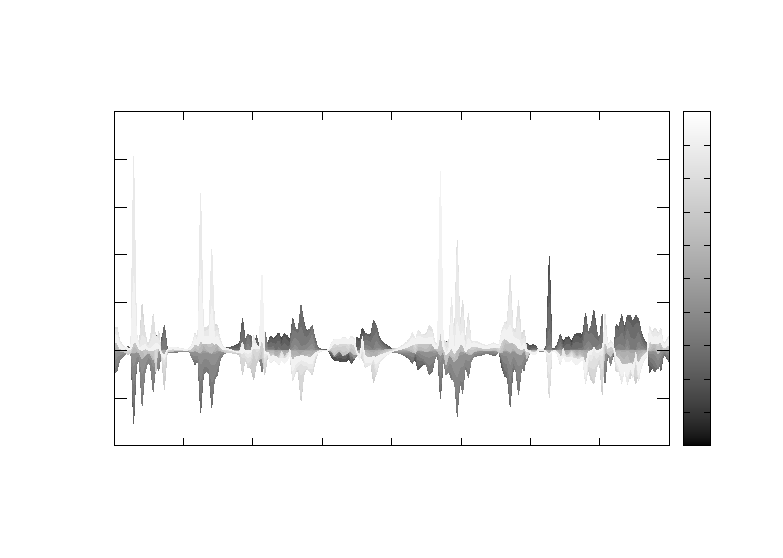
\includegraphics[width={360.00bp},height={252.00bp}]{stt-energy3d-0.2}}%
    \gplfronttext
  \end{picture}%
\endgroup
}
    \resizebox{0.45\textwidth}{!}{% GNUPLOT: LaTeX picture with Postscript
\begingroup
  % Encoding inside the plot.  In the header of your document, this encoding
  % should to defined, e.g., by using
  % \usepackage[cp1252,<other encodings>]{inputenc}
  % \inputencoding{cp1252}%
  \makeatletter
  \providecommand\color[2][]{%
    \GenericError{(gnuplot) \space\space\space\@spaces}{%
      Package color not loaded in conjunction with
      terminal option `colourtext'%
    }{See the gnuplot documentation for explanation.%
    }{Either use 'blacktext' in gnuplot or load the package
      color.sty in LaTeX.}%
    \renewcommand\color[2][]{}%
  }%
  \providecommand\includegraphics[2][]{%
    \GenericError{(gnuplot) \space\space\space\@spaces}{%
      Package graphicx or graphics not loaded%
    }{See the gnuplot documentation for explanation.%
    }{The gnuplot epslatex terminal needs graphicx.sty or graphics.sty.}%
    \renewcommand\includegraphics[2][]{}%
  }%
  \providecommand\rotatebox[2]{#2}%
  \@ifundefined{ifGPcolor}{%
    \newif\ifGPcolor
    \GPcolorfalse
  }{}%
  \@ifundefined{ifGPblacktext}{%
    \newif\ifGPblacktext
    \GPblacktexttrue
  }{}%
  % define a \g@addto@macro without @ in the name:
  \let\gplgaddtomacro\g@addto@macro
  % define empty templates for all commands taking text:
  \gdef\gplbacktext{}%
  \gdef\gplfronttext{}%
  \makeatother
  \ifGPblacktext
    % no textcolor at all
    \def\colorrgb#1{}%
    \def\colorgray#1{}%
  \else
    % gray or color?
    \ifGPcolor
      \def\colorrgb#1{\color[rgb]{#1}}%
      \def\colorgray#1{\color[gray]{#1}}%
      \expandafter\def\csname LTw\endcsname{\color{white}}%
      \expandafter\def\csname LTb\endcsname{\color{black}}%
      \expandafter\def\csname LTa\endcsname{\color{black}}%
      \expandafter\def\csname LT0\endcsname{\color[rgb]{1,0,0}}%
      \expandafter\def\csname LT1\endcsname{\color[rgb]{0,1,0}}%
      \expandafter\def\csname LT2\endcsname{\color[rgb]{0,0,1}}%
      \expandafter\def\csname LT3\endcsname{\color[rgb]{1,0,1}}%
      \expandafter\def\csname LT4\endcsname{\color[rgb]{0,1,1}}%
      \expandafter\def\csname LT5\endcsname{\color[rgb]{1,1,0}}%
      \expandafter\def\csname LT6\endcsname{\color[rgb]{0,0,0}}%
      \expandafter\def\csname LT7\endcsname{\color[rgb]{1,0.3,0}}%
      \expandafter\def\csname LT8\endcsname{\color[rgb]{0.5,0.5,0.5}}%
    \else
      % gray
      \def\colorrgb#1{\color{black}}%
      \def\colorgray#1{\color[gray]{#1}}%
      \expandafter\def\csname LTw\endcsname{\color{white}}%
      \expandafter\def\csname LTb\endcsname{\color{black}}%
      \expandafter\def\csname LTa\endcsname{\color{black}}%
      \expandafter\def\csname LT0\endcsname{\color{black}}%
      \expandafter\def\csname LT1\endcsname{\color{black}}%
      \expandafter\def\csname LT2\endcsname{\color{black}}%
      \expandafter\def\csname LT3\endcsname{\color{black}}%
      \expandafter\def\csname LT4\endcsname{\color{black}}%
      \expandafter\def\csname LT5\endcsname{\color{black}}%
      \expandafter\def\csname LT6\endcsname{\color{black}}%
      \expandafter\def\csname LT7\endcsname{\color{black}}%
      \expandafter\def\csname LT8\endcsname{\color{black}}%
    \fi
  \fi
    \setlength{\unitlength}{0.0500bp}%
    \ifx\gptboxheight\undefined%
      \newlength{\gptboxheight}%
      \newlength{\gptboxwidth}%
      \newsavebox{\gptboxtext}%
    \fi%
    \setlength{\fboxrule}{0.5pt}%
    \setlength{\fboxsep}{1pt}%
\begin{picture}(7200.00,5040.00)%
    \gplgaddtomacro\gplbacktext{%
    }%
    \gplgaddtomacro\gplfronttext{%
      \csname LTb\endcsname%%
      \put(1300,3900){\makebox(0,0)[r]{\strut{}$D$}}%
      \put(936,674){\makebox(0,0){\strut{}$-4$}}%
      \put(1602,674){\makebox(0,0){\strut{}$-3$}}%
      \put(2268,674){\makebox(0,0){\strut{}$-2$}}%
      \put(2934,674){\makebox(0,0){\strut{}$-1$}}%
      \put(3600,674){\makebox(0,0){\strut{}$0$}}%
      \put(4266,674){\makebox(0,0){\strut{}$1$}}%
      \put(4932,674){\makebox(0,0){\strut{}$2$}}%
      \put(5598,674){\makebox(0,0){\strut{}$3$}}%
      \put(6264,674){\makebox(0,0){\strut{}$4$}}%
      \put(3600,344){\makebox(0,0){\strut{}$E(eV)$}}%
      \put(693,917){\makebox(0,0)[r]{\strut{}$-6$}}%
      \put(693,1375){\makebox(0,0)[r]{\strut{}$-4$}}%
      \put(693,1833){\makebox(0,0)[r]{\strut{}$-2$}}%
      \put(693,2291){\makebox(0,0)[r]{\strut{}$0$}}%
      \put(693,2749){\makebox(0,0)[r]{\strut{}$2$}}%
      \put(693,3207){\makebox(0,0)[r]{\strut{}$4$}}%
      \put(693,3665){\makebox(0,0)[r]{\strut{}$6$}}%
      \put(693,4123){\makebox(0,0)[r]{\strut{}$8$}}%
      \put(363,2520){\rotatebox{-270}{\makebox(0,0){\strut{}$\tau$}}}%
      \put(6795,917){\makebox(0,0)[l]{\strut{}$0$}}%
      \put(6795,1237){\makebox(0,0)[l]{\strut{}$0.2$}}%
      \put(6795,1558){\makebox(0,0)[l]{\strut{}$0.4$}}%
      \put(6795,1878){\makebox(0,0)[l]{\strut{}$0.6$}}%
      \put(6795,2199){\makebox(0,0)[l]{\strut{}$0.8$}}%
      \put(6795,2520){\makebox(0,0)[l]{\strut{}$1$}}%
      \put(6795,2840){\makebox(0,0)[l]{\strut{}$1.2$}}%
      \put(6795,3161){\makebox(0,0)[l]{\strut{}$1.4$}}%
      \put(6795,3481){\makebox(0,0)[l]{\strut{}$1.6$}}%
      \put(6795,3802){\makebox(0,0)[l]{\strut{}$1.8$}}%
      \put(6795,4123){\makebox(0,0)[l]{\strut{}$2$}}%
      \put(7257,2520){\rotatebox{-270}{\makebox(0,0){\strut{}$\theta$}}}%
      \put(3600,4453){\makebox(0,0){\strut{}$M=0.3$}}%
    }%
    \gplbacktext
    \put(0,0){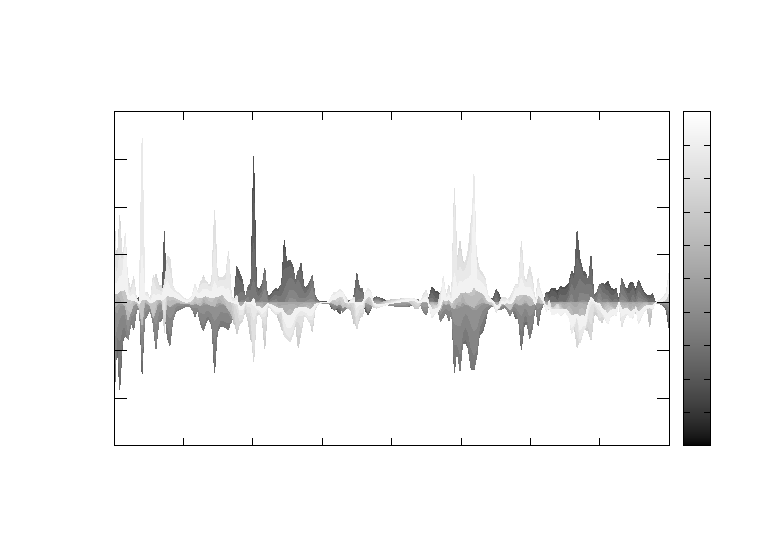
\includegraphics[width={360.00bp},height={252.00bp}]{stt-energy3d-0.3.eps}}%
    \gplfronttext
  \end{picture}%
\endgroup
}
    \caption{الف) گشتاور چرخشی از بوروفن با لبه صندلی، با عرض سلول 4 واحد، برای متغیر مغناطیسی لیدها با توجه به درجه نسبی در جهت z در \lr{E = 0 eV} ترسیم شده است. eV. ب، ج، د) گشتاور چرخشی با مغناطش 0.1، 0.2، 0.3 eV نسبت به انرژی در تمام محدوده زوایای نسبی.}
    \label{fig:stt}
\end{figure*}

\section{مقاله دوم}
% انتقال وابسته به اسپین و گشتاور انتقال اسپین در شیر چرخشی مبتنی بر بوروفن† عرفان نیکان، امیرحسین احمدخان کردبچه، b‡ 
\section{مقدمه}
این مقاله تحلیلی نظری از انتقال و گشتاور انتقال اسپین وابسته به اسپین برای فرومغناطیسی بر پایه بروفن ارائه میکند. اتصال معمولی / فرومغناطیسی این مطالعه بر روی نانوروبانهای بوروفن (BNRs) به عنوان مبنایی برای محاسبات عددی دریچه چرخشی برای هدایت در هر دو پیکربندی که بردارهای مغناطیسی لیدها موازی یا ضد موازی با یکدیگر هستند (به ترتیب پیکربندیهای P و AP)، مقاومت مغناطیسی (MR) تمرکز میکند. و گشتاور انتقال اسپین (STT). رویکردهای فرمالیسم Landauer و تابع گرین غیرتعادلی (NEGF) برای استخراج جریان های تونل زنی وابسته به اسپین در محل اتصال تونل مغناطیسی (MTJ) استفاده می شود. نتایج محاسبات برای BNR زیگزاگ نشان میدهد که رسانایی همیشه بزرگتر از e2/h برای پیکربندی P مغناطیسهای سرب است. برای پیکربندی AP، رسانایی در محدوده انرژی خاص صفر می شود. یک فلات MR کامل برای اتصال در غیاب بی نظمی یافت می شود، که ثابت می کند کاندیدای عالی دریچه چرخشی است. تغییرات STT با انرژی فرمی، زاویه نسبی بین دو مغناطیس الکترود، برای قدرت های مختلف مغناطیس فرومغناطیسی مورد مطالعه قرار گرفته است. ولتاژ بایاس STT در واحد، به عنوان تابعی از انرژی فرمی، به طور قابل توجهی در انرژی نقطه دیراک کاهش می یابد. یک الگوی نوسانی سینوسی را می توان به وضوح در STT در ولتاژ بایاس واحد V در مقابل زاویه بین مغناطش دو الکترود مشاهده کرد، که با افزایش M تقویت می شود. بوروفن دارای خواص منحصر به فردی از جمله چگالی کم و سختی بالا، مقاومت در برابر حرارت و رسانایی الکتریکی است که آن را به یک نامزد امیدوارکننده برای اسپین ترونیک تبدیل می کند. این مقاله تجزیه و تحلیل جامعی از خواص بوروفن وابسته به اسپین و کاربردهای بالقوه آن در اسپینترونیک ارائه می دهد.

\section{رسانش کوانتومی اسپین}
اسپینترونیک معمولاً به پدیده‌هایی اطلاق می‌شود که در آن اسپین الکترون‌ها در یک محیط حالت جامد نقش تعیین‌کننده را ایفا می‌کند. به معنای محدودتر اسپینترونیک یک زمینه تحقیقاتی نوظهور در الکترونیک است: دستگاه های اسپینترونیک بر اساس کنترل اسپین الکترونیک یا کنترل الکتریکی و نوری اسپین یا مغناطیس هستند. در حالی که اسپینترونیک فلزی قبلاً جایگاه خود را در صنعت رایانه پیدا کرده است - سیستم‌های مقاومت مغناطیسی غول‌پیکر به عنوان سرهای خواندن دیسک استفاده می‌کنند - اسپینترونیک نیمه‌رسانا هنوز پتانسیل کامل خود را نشان نداده است. این بررسی مضامین منتخب اسپینترونیک نیمه هادی را ارائه می کند، مفاهیم مهم ترابرد درون اسپین، تزریق اسپین، کوپله اسپین-شارژ سیلسبی-جانسون، و تونل زنی وابسته به اسپین، همچنین آرامش اسپین و دینامیک اسپین را معرفی می کند. اساسی ترین برهمکنش وابسته به اسپین در نیمه هادی های غیر مغناطیسی، جفت شدن اسپین-مدار است. بسته به تقارن‌های کریستالی مواد، و همچنین ویژگی‌های ساختاری هتروساختارها مبتنی بر نیمه‌رسانا، کوپلینگ مداری اسپین شکل‌های عملکردی متفاوتی به خود می‌گیرد و زمین بازی خوبی از همیلتونی‌های مدار چرخشی موثر ایجاد می‌کند. هامیلتونی‌های مؤثر برای مرتبط‌ترین کلاس‌های مواد و ناهمساختارها در اینجا از توضیحات ساختار نوار الکترونیکی واقعی مشتق شده‌اند. اکثر سیستم های دستگاه های نیمه هادی هنوز مفاهیم نظری هستند و منتظر نمایش های تجربی هستند. مروری بر منتخب پیشنهادی، و چند دستگاه نشان‌داده‌شده، با شرح دقیق دو کلاس مهم ارائه می‌شود: ساختارهای تونلی تشدید مغناطیسی و دیودها و ترانزیستورهای مغناطیسی دوقطبی. با توجه به اهمیت مواد نیمه هادی فرومغناطیسی، بحث مختصری در مورد نیمه هادی های مغناطیسی رقیق شده گنجانده شده است. در بیشتر موارد، ارائه به سبک آموزشی است، که فرمالیسم نظری ضروری را در سطحی قابل دسترس معرفی می‌کند، با تصاویری شبیه به مطالعه موردی از نتایج تجربی واقعی، و همچنین با مرور مختصر دستاوردهای اخیر مرتبط در این زمینه.

ساختار CIP، و خلأ این محاسبات مختلف، از جمله هدایت P و AP و MR و STT، در ساختار CPP دریچه چرخشی برای β12-بوروفن 74 احساس میشود. این مقاله به بررسی تحلیل نظری انتقال وابسته به اسپین و انتقال اسپین میپردازد گشتاور برای اتصال FM/normal/FM مبتنی بر بوروفن. لازم است تا جریان های تونل زنی وابسته به چرخش در MTJ با استفاده از یک چارچوب مناسب برای بهبود توصیف نظری مقاومت مغناطیسی فرموله شود. برای این منظور، فرمالیسم لنداور 75، بر اساس تابع گرین غیرتعادلی (NEGF) 76، به عنوان یک رویکرد قابل قبول و پرکاربرد معرفی شده است. در اینجا ابتدا رسانایی بوروفن برای هر دو پیکربندی P و AP محاسبه میشود و رسانایی صفر در برخی انرژیها در پیکربندی AP و رسانایی غیر صفر در پیکربندی P مشاهده میشود. این ویژگی حالت های ON و OFF را برای استفاده در سوئیچ ایجاد می کند. پراکندگی ترکیبی وابسته به اسپین ممکن است دلیل رسانایی صفر را در پیکربندی AP توضیح دهد و فیلتر انتخاب باند را می توان با استفاده از برابری زیر باندها نشان داد. علاوه بر این، بر این اساس، نوسانات جزئی و مکرر برخی از انرژی ها روشن می شود. در صورت عدم وجود اختلال، یک فلات MR کامل برای اتصال یافت می شود که ثابت می کند کاندیدای عالی دریچه چرخشی است. تغییرات گشتاور انتقال اسپین با انرژی فرمی و زاویه نسبی بین دو مغناطیس الکترود در شدت های مغناطیسی فرومغناطیسی مختلف بررسی شده است. محاسبات نشان می دهد که ولتاژ بایاس STT در واحد (e/4π)، به عنوان تابعی از انرژی فرمی، به طور قابل توجهی در نزدیکی انرژی نقطه دیراک کاهش می یابد. علاوه بر این، یک الگوی نوسانی سینوسی را می توان در STT در ولتاژ بایاس واحد V در مقابل زاویه بین دو مغناطش الکترود تشخیص داد که با افزایش M تشدید می شود. در نهایت، به منظور درک صحیح سیستم، G به عنوان تابعی از زاویه نسبی بین دو مغناطش الکترود، و همچنین در اطراف انرژی نقطه دیراک بررسی میشود. بقیه مطالعه به شرح زیر تنظیم شده است: در بخش 2، مدل و فرمولی که بر اساس آن محاسبات انجام می شود را مورد بحث قرار می دهیم. بخش 3 یافته های عددی را برای رسانایی وابسته به چرخش، MR، و STT برای نمونه های لبه زیگزاگ و صندلی راحتی ارائه می دهد. در بخش 4، مقاله با یک بحث مفصل و یک نتیجه گیری کوتاه به پایان می رسد.

\section{دریچه اسپینی:}
یکی از پیشرفت‌های مهم در دو دهه اخیر، دریچه اسپینی  است، دستگاهی با دو اتصال مغناطیسی (شکل 14.1) اگر در یک جهت مغناطیسی شوند (پیکربندی موازی، P)، مقاومت حاصل از مغناطیسی شدن آنها کمتر است. در جهت مخالف (پیکربندی پاد موازی، AP). از زمان اولین نمایش خود در سال 1988، به سرعت به عنوان یک دستگاه خواندن برای درک اطلاعات ذخیره شده در یک حافظه مغناطیسی کاربرد پیدا کرد و این کشف با جایزه نوبل در سال 2007 شناخته شد.
\begin{figure*}[!ht]
  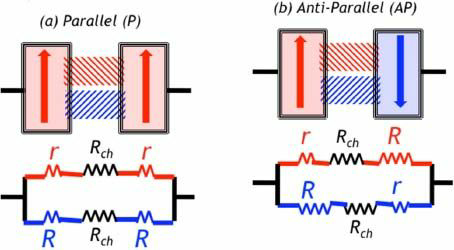
\includegraphics[width=0.5\linewidth]{./figures/spinvalve.png}
  \caption{دریچه چرخشی: (الف) پیکربندی موازی (P). (ب) پیکربندی ضد موازی (AP).}
\end{figure*}
تا اینجا ما فقط به اسپین به عنوان بخشی از "ضریب تبهگنی ، g" اشاره کرده‌ایم (بخش 5.4)، ایده این است که حالت‌های الکترونیکی همیشه به صورت جفت می‌آیند که یکی مربوط به هر اسپین است. همانطور که در شکل 14-1 انجام دادیم، می‌توانیم اینها را «بالا» و «پایین» یا «چپ» و «راست» یا حتی «قرمز» و «آبی» بنامیم. توجه داشته باشید که این دو اسپین از نظر مکانی از هم جدا نیستند، حتی اگر کانال قرمز و آبی را برای وضوح از هم جدا کرد.

معمولاً دو کانال یکسان هستند و می توانیم رسانایی ناشی از یک را محاسبه کنیم و به یاد داشته باشیم که در دو ضرب کنیم. اما در دستگاه‌های دریچه اسپین،اتصال ها مغناطیده هستند که با دو کانال اسپین برخورد متفاوتی می‌کنند و عملکرد یک دریچه اسپینی با فرض اینکه که هر کانال اسپینی مقاومت رابط  متفاوتی، بسته به مغناطش اتصال، دارد،که یا موازی (اسپین اکثریت) یا پاد موازی (اسپین اقلیت) با مغناطش اتصال ها است.

اگر مقاومت رابط را برای اسپین های اکثریت r و برای اسپین های اقلیت R (r < R) فرض کنیم، می توانیم نمایش های مدار ساده ای را برای پیکربندی های P و AP همانطور که نشان داده شده است ترسیم کنیم، با Rch نشان دهنده مقاومت کانال است. سپس تئوری مدارهای ابتدایی مقاومت پیکربندی موازی را به ما می دهد

همانطور که در شکل 1 نشان داده شده است، یک نانوروبان بوروفن غیر مغناطیسی (BNR) با دو سر (به عنوان ناحیه مرکزی) که بین دو نانوروبان بوروفن FM نیمه نامتناهی (به عنوان دو الکترود) قرار گرفته است، یک دستگاه شیر چرخشی را تشکیل می دهد. شایان ذکر است که حامل های بار بوروفن به طور کلی قطبش اسپینی نیستند و خاصیت مغناطیسی توسط یک بستر فرومغناطیسی عایق (با رشد بوروفن بر روی عایق FM) به سرنخ های بوروفن تزریق می شود. از آنجایی که استفاده از میدان مغناطیسی می تواند برای شکستن تقارن معکوس زمانی مورد استفاده قرار گیرد، میدان تبادل ایجاد شده از طریق اثر مجاورت ناشی از یک بستر عایق فرومغناطیسی، باعث می شود که زمان معکوس یا تقارن اسپین شکسته شود. بر خلاف روشهای جایگزین برای شکستن TRS، مانند دوپینگ 79،80 اتم فلزات واسطه و حجمدهی اتمی 81،82، این تکنیک یک دستکاری برهمکنش کوتاه برد خارجی است که تأثیری بر تحرک الکترون در کاربردهای الکترونیکی ندارد. اگر ناحیه هسته دارای طول L و دارای N اتم در عرض باشد، این ناحیه دارای 5 N (2L + 1) اتم است. مجموع هامیلتونی سیستم شیر چرخشی به صورت زیر بدست می آید:
جایی که EL، ER و EC به ترتیب انرژیهای موجود در نانوروبانهای بوروفن در لیدهای چپ و راست و ناحیه مرکزی هستند که میتوانند با ولتاژ گیت تنظیم شوند، بسته به محل نقطه شبکه، همانطور که در نشان داده شده است. میز 1. a† iσ(aiσ) عملگرهای ایجاد (نابودی) الکترون در محل i با اندیس اسپین (σ) هستند. ML و MR مغناطشهای الکترودهای FM چپ و راست هستند و θ زاویه بین جهتگیریهای ML و MR است. جریان الکتریکی که از سیستم عبور می کند را می توان با استفاده از رویکرد تابع گرین غیرتعادلی مشخص کرد.
در جایی که ΣLσ(Rσ) تابع انرژی خود عقب مانده سرب چپ (راست) در فضای اسپین 48 است. توجه داشته باشید که اثر الکترودهای نیمه نامتناهی بر همیلتونی سیستم با استفاده از اصطلاحات خود انرژی توصیف شده است. انرژی های خود به صورت تکراری 83،84 محاسبه می شوند. اکنون رسانایی کل برای اتصال را می توان به صورت زیر بدست آورد:

\begin{equation}
  \begin{aligned}
  & P:{{\left[ \frac{1}{2r+{{R}_{ch}}}+\frac{1}{2R+{{R}_{ch}}} \right]}^{-1}} \\ 
 & AP:\frac{r+R+{{R}_{ch}}}{2}  
  \end{aligned}
\end{equation}
ماهیت دستگاه دریچه اسپینی تفاوت بین RP و RAP است و ما انتظار داریم زمانی که مقاومت کانال ناچیز است و همه چیز تحت سلطه رابط ها است، این موضوع بیشتر برجسته باشد. شکل 14.2 تغییر مقاومت مغناطیسی (MR، تعریف شده در زیر) را به عنوان تابعی از مقاومت کانال (در هر اسپین) Rch نرمال شده به r+R با فرض P=0.5 نشان می‌دهد. توجه داشته باشید که وقتی Rch نرمال شده بیش از مثلاً ~5 افزایش یابد، MR به سرعت از بین می رود.


استفاده از مواد دوبعدی گرافن و سیلیسین به عنوان پایه شیرهای اسپین مورد توجه قرار گرفته است. بوروفن به عنوان یکی دیگر از مواد دوبعدی با خواص جدیدش کمتر برای این منظور مورد مطالعه قرار گرفته است. در این مقاله از بوروفن نیز برای همین منظور استفاده خواهیم کرد. با توجه به عملی متعدد نام، شکل 4 مقاومت منگنه (MR) β12-بوروفن در صندلی راحتی و لبه های زیگزاگ. کاربردهای cal در دستگاه هایی مانند سوئیچ ها، هدهای دیسک سخت و MRAM و همچنین STT-MRAM ها و اهمیت پارامترهایی مانند رسانایی (موازی و ضد موازی)، MR و STT در طراحی یک شیر اسپین، مطالعه این خواص در بوروفن مورد توجه قرار خواهد گرفت. نتیجه محاسبات عددی برای CPP برای پیکربندی های موازی (P) و ضد موازی (AP) متشکل از یک نانوروبان با عرض چهار سلول واحد در شکل 1 نشان داده شده است. در تمام محاسبات، الکترودهای چپ و راست به عنوان یک کانال بوروفن با مغناطیسی برابر، به صورت ML = MR = M در نظر گرفته می شوند. خاصیت مغناطیسی توسط یک بستر فرومغناطیسی عایق (با رشد بوروفن بر روی عایق FM) به سرنخ های بوروفن تزریق می شود. زاویه θ جهت گیری کلی مغناطش لیدهای راست و چپ را نسبت به یکدیگر تعیین می کند، در حالی که حالت خاص θ = 0 (π) به ترتیب مغناطش موازی (یا ضد موازی) لیدهای چپ و راست را نشان می دهد.

% طیفهای انتقال نانوروبان بوروفن خالص، در دو لبه زیگزاگ و صندلی صندلی (BNRs)، ساختار پله مانند معروفی را نشان میدهند. تعداد زیر باندهای انرژی در هر انرژی ارتفاع پله مربوطه را تعیین می کند. علاوه بر این، بر خلاف نانوروبانهای گرافن (GNRs)، تعداد کانالهای رسانش در انرژی فرمی در نانوروبانهای بوروفن 85 ثابت نمیماند و با افزایش عرض نانوروبانها، تعداد کانالها افزایش مییابد که در نانوروبانهای زیگزاگ بیشتر از نانوروبانهای صندلی صندلی قابل مشاهده است. 75. برخلاف گرافن که رسانایی آن در انرژی فرمی (در اینجا E = 0 eV ) به عرض نانوروبان بستگی ندارد، رسانایی بوروفن در انرژی فرمی با تغییر عرض نانوروبان تغییر میکند. دلیل این امر را می توان در تفاوت تعداد زیر باندهای بین گرافن و بوروفن جستجو کرد که از انرژی فرمی صفر عبور می کنند و این به دلیل وجود یک اتم اضافی در مرکز سلول واحد در بوروفن است. بنابراین، میتوان گفت که اتم مرکزی داخل سلول واحد در بوروفن، وابستگی کانالهای رسانایی به عرض نانوروبان در انرژی فرمی را به حساب میآورد. ابرسلول ها را می توان با نام اتم لبه بالا و پایین آنها شناسایی کرد، مانند ZNBR-cd که به اتم a-c در لبه بالایی و اتم a-d در لبه پایین ختم می شود. محاسبات ما نشان می دهد که، علیرغم داشتن یک شکاف باند بسیار باریک، ZNBR-cd عرض 8.8A ویژگی های فلزی را نشان می دهد. در بسیاری از مطالعات قبلی، ابرسلول های در نظر گرفته شده در محاسبات با یک سلول در هر دو طرف 75،77 خاتمه می یافتند. در تحقیق حاضر نیز به همین صورت انجام شده است. از آنجایی که هر ABNR می تواند به b-d(ac-a) ختم شود، که نام آن را α(γ) می گذاریم، ما چهار نوع ابرسلول ABNR داریم که یکی از آنها ABNR-αα است.

محاسبات ما نشان می دهد که برخلاف ZBNR ها، ABNR ها رفتار نیمه هادی یا فلزی را بسته به عرض روبان W از خود نشان می دهند، به طوری که برای عرض های بزرگتر از مقدار بحرانی Wc = 11.08 Å، 86 رسانایی غیر صفر را می توان یافت، در حالی که سیستم رفتار می کند. مانند یک نیمه هادی برای عرض های کوچکتر از Wc. حالت های لبه را می توان در شکاف انرژی نیمه هادی ها و همچنین شکاف باند محلی هادی ها مشاهده کرد. در نتیجه، حتی اگر معمولاً از نیمه هادی ها استفاده می شود، حالت های صفر را می توان در عرض های مشخص شده مناسب ایجاد کرد. اعمال میدان مغناطیسی تبادل درون صفحه ای باعث می شود هامیلتونین اسپین قطبی شده با عملگر اسپین S رفت و آمد نداشته باشد و در این حالت اسپین الکترون دیگر ثابت حرکتی در سیستم نخواهد بود. این بدان معناست که حالت اسپین ممکن است در جهت انتقال تغییر کند. در واقع، در نتیجه برهمکنش اسپین الکترون با میدان مغناطیسی تبادل درون صفحه، چرخش اسپین رخ میدهد، به عنوان مثال، الکترونی که با حالت اسپینآپ وارد کانال میشود ممکن است کانال را به صورت اسپین ترک کند. حالت پایین هنگامی که یک میدان مغناطیسی به دلیل وجود یک زیرلایه عایق فرومغناطیسی روی لیدها اعمال می شود، یک میدان مغناطیسی خارج از صفحه به شیرهای اسپین وارد می شود. با توجه به بررسی های ما، در این مورد، رسانایی نسبت به لیدهای غیر مغناطیسی تغییراتی را نشان می دهد. تجزیه و تحلیل دقیق این تغییرات برای درک آنها و دانستن منشأ آنها یک مسئله کلیدی برای طراحی شیرهای اسپین قابل اجرا و بهره برداری کامل از پتانسیل آنها است. در نتیجه تغییر خواص مغناطیسی لیدها از حالت غیر مغناطیسی به مغناطیسی شده، تغییر در تعداد و عرض پلاتوها ایجاد می شود. با این حال، با افزایش مغناطش در الکترودها، انحراف از ساختار پله مانند به وضوح مشاهده می شود. دلیل این امر را می توان بر اساس خروج برخی از سطوح انرژی از ترانس تشریح کرد.
دلیل این امر را می توان بر اساس خروج برخی از سطوح انرژی از شکل. عرض سلول 4 واحد، برای متغیر مغناطیسی لیدها با توجه به درجه نسبی در جهت z در E = 0 eV . ب، ج، د) گشتاور چرخشی با مغناطش 0.1، 0.2، 0.3 eV نسبت به انرژی در تمام محدوده زوایای نسبی پنجره انرژی ماموریت به دلیل جدا شدن سطوح انرژی در الکترودها، همراه با بقای برابری زیر باند انرژی به عنوان یکی دیگر از موارد دیگر. مکانیسم های موثر بر انتقال جداسازی اسپین ناشی از اثر زیمن، ساختار باند را تغییر میدهد و در یک پنجره انرژی، تعداد زیر باندها در هر دو حالت لیدهای مغناطیسی و غیر مغناطیسی تغییر میکند. در ادامه، انحرافات رسانایی در لیدهای مغناطیسی شده را در مقایسه با غیر مغناطیسی شده توضیح می دهیم که نمودارها رسانایی برای مغناطیس های مختلف M را نشان می دهند و آنها را با حالت M=0 مقایسه می کنند. یکی از تغییرات از محفظه سربی غیر مغناطیسی به حالت مغناطیسی، تغییر در تعداد و عرض صفحات در نمودار رسانایی است که با افزایش مغناطیسی رخ می دهد. فلات ها در نمودار انتقال در محدوده انرژی دیده می شوند که تعداد زیر باندهای درگیر در فرآیند انتقال ثابت است و زمانی که تعداد زیر باندها در هر انرژی تغییر می کند، رسانایی نیز تغییر می کند. بنابراین، عرض پلاتوها در نمودار رسانایی به تفاوت بین زیر باندهای انرژی بستگی دارد. با توجه به پایه دو اتمی موادی مانند گرافن، سیلیسن و غیره، فرورفتگی زیر باندها حتی زمانی که تعامل تبادلی در نظر گرفته شود، رخ نمی دهد. دو نوع فاصله بین باندی دیده می شود. اولی فاصله بین دو زیر باند اسپینی با تراز مخالف یکسان است که برابر با 2M است و دیگری فاصله بین باند چرخشی N - 1 و زیر باند چرخشی N-امین است. در بوروفن، به دلیل وجود یک اتم اضافی که در مرکز شش ضلعی قرار دارد، سطح انرژی ناشی از برهمکنش تبادلی تورفتگی وجود دارد. به همین دلیل، تنوع فاصله بین زیر باندها بسیار بیشتر از قبل است که با تنوع عرض پلاتوها همراه است و در رسانش شکل 2.b نیز تایید شده است. بنابراین، برهمکنش مبادله به دلیل تغییری که در فاصله بین باند ایجاد می کند، الگوی رسانایی گام مانند را بیشتر تغییر می دهد. یکی از اولین انحرافاتی که در لیدهای مغناطیسی نشان داده شده در شکل 2.a، b در مقایسه با حالت غیر مغناطیسی یافت می شود، وجود مراحل یا نوسانات در رسانایی با مقادیر کوچکتر از G0 (G0 = e2/h) در هر پیکربندی است. . علت این پدیده عدم تطابق بین برابری زیر باندهای کانال و برابری زیر باندهای الکترودهایی است که مقدار تونل آنها در مقایسه با حالت غیر مغناطیسی کمتر از یک G0 است. این بدان معنی است که علاوه بر تعداد زیر باندها در آن پنجره انرژی، برابری زیر باندها نیز در فرآیندهای تونل زنی و انتقال الکترون بسیار مهم است. این متعاقبا باعث ایجاد فلات هایی با مقادیر فرد (که می توان گفت دارای خواص نیمه فلزی هستند) یا مقادیر نیمه صحیح می شود. البته برخلاف گرافن، این نوع تونل زنی الکترونی که در گرافن فقط در EF <M دیده می شود، در بوروفن در سراسر طیف انرژی دیده می شود.
در غیاب هر گونه تعاملی که نرخ تونل زنی را کاهش دهد، با توجه به سهم  G0 با توجه به هر زیر باند در پنجره انرژی (همانطور که در مورد P مشاهده می شود)، وجود هر فلات با ارتفاع 2G0 در نمودار هدایت، میزان کل تونل زنی در پنجره انرژی را نشان می دهد. در مورد AP، سرعت کامل تونلزنی در دو موقعیت اتفاق نمیافتد: 1. وقتی دو زیر باند مرتبط با دو الکترود برابری مخالف دارند، علیرغم عدم وجود شکاف انرژی در ساختار نوار، رسانش صفر خواهد بود. در پیکربندی AP، شماره گذاری باندهای انرژی در الکترودهای چپ و راست با یکدیگر متفاوت است و برابری باندهای فرعی نیز مخالف است. یعنی زیر باندهایی با اعداد یکسان در دو الکترود دارای برابری مخالف هستند. در این صورت بر اساس قاعده انتخاب برابری، تونل زنی ممنوع خواهد بود، یعنی در طول فرآیند تونل زنی، الکترون با برابری زوج در الکترود چپ نمی تواند به الکترون با برابری فرد در الکترود سمت راست تبدیل شود و بنابراین با وجود عدم وجود شکاف باند، رسانایی صفر خواهد بود. (برای چنین الکترونی، حتی اگر شکاف نواری صفر باشد، رسانش باز هم صفر خواهد بود.) تعداد زیر باندها به تعداد اتم های ابرسلول بستگی دارد و در غیاب میدان مغناطیسی، دارای اسپین دوگانه هستند. انحطاط در الکترودها، زمانی که بستر مغناطیسی یک میدان مغناطیسی به صفحه اعمال می کند، تقسیم سطوح انرژی رخ می دهد. بنابراین تعداد زیر باندها دو برابر می شود. از سوی دیگر، می دانیم که زیر باندها دارای تقارن برابری به دلیل ساختار متقارن ماتریس Hk هستند که به تعداد آنها بستگی دارد. یعنی زیر باندهای 0، 2، 4 و . . . زوج هستند و زیر باندهای 1، 3، 5 و . . . نیز عجیب و غریب هستند. وقتی زیر باندها تقسیم می شوند، این شماره گذاری دوباره از ابتدا انجام می شود. بنابراین، در پیکربندی AP، به عنوان مثال، زیر باند 8 به دو باند 8 به بالا و 8 پایین تقسیم می شود که ترتیب آنها در الکترود مخالف برعکس است. با توجه به شماره گذاری مجدد به برابری، زیر باندهای با تعداد یکسان در دو الکترود با مغناطش مخالف، برابری مخالف خواهند داشت و بنابراین در این حالت تونل سازی صورت نمی گیرد زیرا هر زمان که اسپین های زیر باند در دو الکترود مخالف یکدیگر باشند، تونل زنی الکترونی ممنوع است. به یکدیگر. این بدان معناست که یک الکترون با برابری زوج در الکترود چپ، در طول فرآیند تونلزنی، الکترون برابری فرد را در الکترود سمت راست ایجاد نمیکند، که منجر به رسانایی صفر میشود، حتی در صورت عدم وجود شکاف نواری در آن محدوده انرژی. 2. در شرایطی که عدم تطابق برابری در زیر باندهای بین الکترودها و کانال مرکزی رخ می دهد. در این حالت سهم تونل سازی در هر زیر باند کمتر از G0 و در نتیجه رسانایی کمتر از 2 G0 خواهد بود. (مثلاً محدوده انرژی -1 eV تا 0.0 eV برای M = 0.3 eV در شکل 3.e. در برخی از انرژی ها در محدوده -0.60 eV تا -0.38 eV، همانطور که در شکل 2.a مشاهده می شود، رسانایی برای M = 0.2 eV صفر می شود، با توجه به اینکه نمودار ساختار نواری هیچ شکاف نواری در این محدوده ندارد، همانطور که در شکل 3.a,b,c مشاهده می شود، دلیل رسانایی صفر را می توان توضیح داد. بر اساس قوانین انتخاب برابری در تونل زنی، در واقع، به طور دقیق تر، در این حالت، هماهنگی بین تعداد زیر باندهای این پنجره انرژی و برابری آنها به گونه ای است که این صفرهای رسانایی ایجاد می شوند، اما لزوماً همه صفرهای رسانایی ایجاد نمی شوند. از این هماهنگی حاصل می شود و این پنجره انرژی یک مثال است.همچنین در یک ABNR با پیکربندی P حاوی چهار سلول واحد در عرض (شبیه به پیکربندی AP)، عرض فلات کاهش می یابد و ساختار رسانایی پله مانند حفظ می شود. رسانایی صفر در انرژی های -0.6 eV و 0.38 eV و 0.63 eV تا 0.83 eV (برای M = 0.2 eV)، 0.35 eV تا 0.56 eV (برای M = 0.3 eV) دیگر رخ نمی دهد. همانطور که مشاهده می شود، علیرغم شرایط مشابه در پیکربندی های P و AP شکل 3.d، e (مانند نوع لبه ها، پنجره های انرژی و مغناطیس شدن لیدها)، دلیل رسانایی غیر صفر در پیکربندی P این است که برخلاف پیکربندی AP، قانون انتخاب برابری حفظ می شود. البته، هنوز هم می توان رفتار نیمه فلزی را برای این پیکربندی در انرژی های حدود 0.3 eV (با مغناطیسی M = 0.3 eV) و -0.6 eV (با مغناطیسی M = 0.2 eV) در نظر گرفت. نوسانات کوچک در رسانایی شکل 2.c,d ناشی از عدم تطابق برابری توابع موج عرضی در الکترودها و کانال است. در این حالت، انتقال الکترون انجام میشود، اما با سرعت کمتری نسبت به حالتی که برابری دو باند فرعی در الکترود و کانال یکسان است (که در مورد ما یک G0 است). نانوروبانهای بوروفن زیگزاگ عموماً خواص رسانایی بیشتری از خود نشان میدهند که با بررسی ساختار نواری آنها و مقایسه آن با نانوروبانهای بوروفن صندلی راحتی قابل مشاهده است. اگرچه نوسانات رسانایی را در اینجا نیز می توان مشاهده کرد که ناشی از عدم تطابق برابری حالات در الکترودها و کانال است، رسانایی با افزایش مغناطیس تغییرات زیادی را نشان نمی دهد. همچنین رسانایی صفر ظاهر نمی شود. تفاوت بین پیکربندیهای P و AP در بوروفن زیگزاگ بسیار کمتر از بوروفن صندلی صندلی است، که متعاقباً باید به این نتیجه برسد که بوروفن زیگزاگ در دستگاه شیر چرخشی ارزش کمتری خواهد داشت. بررسی MR یک معیار مهم برای امکان استفاده از یک دستگاه به عنوان یک شیر چرخشی مناسب فراهم می کند. این بدان معناست که اگر یک دستگاه علاوه بر داشتن تغییرات قابل توجهی در رسانایی بین پیکربندیهای P و AP دارای مقاومت مغناطیسی بالایی باشد، میتواند کاندیدای بالقوه خوبی برای یک دستگاه شیر چرخشی باشد.

\section{مغناطومقاومت:}
اثر MR را می توان با استفاده از یک دستگاه شیر چرخشی 12 تجزیه و تحلیل کرد. بسته به اینکه کانال ساندویچ شده در شیر چرخشی فلزی یا عایق است، پدیده مقاومت مغناطیسی (GMR) و مقاومت مغناطیسی تونل (TMR) را می توان مشاهده کرد. 13. علاوه بر توصیف فیزیک پشت رفتار MR، بررسی نظری MR همچنین نقش پارامترهای مختلف موثر در رفتار MR 14 را مطالعه میکند.

با توجه به تعریف MR، بدیهی است که مقدار آن برای M = 0 eV باید صفر باشد، زیرا در این حالت، هیچ تفاوتی بین تنظیمات AP و P وجود ندارد. در واقع مقادیر غیر صفر M دو پیکربندی ذکر شده را از یکدیگر متمایز می کند. همانطور که در شکل 4.a مشاهده می شود، زمانی که M = 0.05 eV، یک ساختار فلات کامل را می توان مشاهده کرد. در این مورد، پیکربندی A یک نارسانا با رسانایی صفر است، در حالی که پیکربندی P خواص رسانایی خوبی را با مقدار G0 نشان میدهد. ما می دانیم که وقتی فلات های 100\% در نمودار MR وجود دارد، رسانایی در AP صفر می شود و رسانایی برای پیکربندی P به اندازه کافی بزرگ است، که از شکل 4.b مشخص است، که حدود یک G0 است. در مقایسه با گرافن و سیلیسین، قله های MR در بوروفن بسیار نامنظم تر و کمتر شبیه هیستوگرام هستند، همانطور که در شکل 4.a نشان داده شده است. برای M = 0.05 eV، یک فلات 100٪ (فلات کامل) در انرژی 3.8 eV رخ می دهد که در آن عرض فلات با افزایش M به 0.1 eV افزایش می یابد. که با دانش ما در مورد تغییر عرض فلات با M مطابقت دارد.
همانطور که در شکل 2.a مشاهده می شود، تعداد پنجره های انرژی با رسانایی صفر در پیکربندی AP در M = 0.2 eV و M = 0.3 eV بسیار بیشتر است، و بنابراین تعداد فلات های 100\% نیز بیشتر است. برخلاف گرافن و سایر مواد دوبعدی، که 100 درصد فلات ها (فلات کامل) در اطراف انرژی نقطه دیراک EF = 0 eV قرار دارند، در بوروفن، 100 درصد فلات ها در تمام انرژی ها رخ می دهند و شکل هیستوگرام پایین تری را نشان می دهند. این پدیده را می توان یک مزیت برای بوروفن در نظر گرفت زیرا کاربرد مقاومت مغناطیسی گرافن در سوئیچینگ به انرژی خاص (انرژی نقطه دیراک) محدود می شود، در حالی که چنین محدودیتی برای بوروفن وجود ندارد. یعنی انتخاب های بیشتری در محدوده انرژی برای تنظیم سایر پارامترهای لازم برای ساخت دستگاه ها وجود دارد و ما محدود به انرژی خاصی نیستیم. تغییر 100٪ عرض فلات در بوروفن در درجه اول به دلیل رسانایی AP صفر است، که متعاقباً بر اساس فاصله زیر باندها و قانون انتخاب برابری، همانطور که در بخش های قبلی بیان شد، به دست می آید. همانطور که مشخص است، از آنجایی که رسانایی دارای صفرهایی با عرض بزرگتر است (یعنی رسانایی در محدوده انرژی بزرگتر صفر است)، همان عرض انرژی با رسانایی صفر در نمودار MR با فلات ها با مقدار یک منعکس می شود. بنابراین، توصیف عرض فلات نمودار MR کاملاً به دو عامل تعیین کننده صفرهای رسانایی بستگی دارد. علت دره ها در نمودار MR به فاصله کمتر بین زیر باندها در هر مغناطیس نسبت داده می شود که منجر به نزدیک بودن رسانش در دو پیکربندی به یکدیگر می شود. در نتیجه، می توان نتیجه گرفت که رسانایی در آن نقاط تا حدودی مستقل از جهت گیری الکترودها است. 
\section{ترابرد گشتاور اسپینی}

گشتاور انتقال اسپین (STT) به دلیل استفاده از اسپین الکترون در فناوری ذخیره سازی و حسگرها توجه بسیاری از محققین را به خود جلب کرده است. رالف و استایلز به صورت نظری فیزیک STT را در دستگاه های مغناطیسی ارائه کردند. STT با استفاده از مدل اسپین دیفیوژن 17 و ژانگ و همکاران. مکانیسم سوئیچینگ مغناطیسی را با گنجاندن برهمکنش مبادله 18 مورد بررسی قرار داد. با توجه به امکان استفاده از شیرهای اسپین در دستگاه های الکتریکی، مغناطیسی و اسپینی، مواد دوبعدی (2D) در سال های 19-22 بیشتر و بیشتر مورد توجه قرار گرفته اند. متغیرهای ساختاری متعددی، مانند اندازه پوسته، ضخامت، شکل لبه، عیوب ذاتی، اتمهای انتهایی لبه، و سایر متغیرهای 20،23-25، میتوانند بر ویژگیهای یک ماده تأثیر بگذارند. قابلیت تبدیل مواد با لایه دوبعدی به نانوروبانها، علاقه تحقیقاتی را برانگیخته است، زیرا این مواد به دلیل خواص مغناطیسی منحصر به فرد در ساختار الکترونیکی خود، پتانسیل تبدیل شدن به مواد الکترونیکی جدید را دارند. استفاده از نانو نوارها در الکترونیک اسپین یک موضوع تحقیقاتی رایج است. به دلیل ویژگیهای استثنایی وابسته به چرخش، از جمله زمان استراحت چرخش فوقالعاده طولانی و طول انتشار چرخش، جفتشدن مدار چرخشی راشبا (SOC)، قفل شدن دره چرخشی، و اثر هال اسپین کوانتومی، مواد دوبعدی مانند گرافن 26، فسفر سیاه (BP) 27، دی کالکوژنیدهای فلزات واسطه (TMDCs) 28، و سیلیسین 29 یک پلت فرم عالی برای تحقیقات اسپینترونیک 30-33 ایجاد کرده اند. Brey و Fertig 34 MR یک اتصال FM/گرافن/FM را در حد عرض بی نهایت با استفاده از مفهوم اتصال محکم بررسی کردند. از آنجایی که رسانایی به طور ضعیف تحت تأثیر جهت گیری های مغناطیسی نسبی سیم های FM قرار می گیرد، آنها دریافتند که MR نسبتاً کم است. یک دستگاه قابل مقایسه با دو لید FM توسط دینگ و همکاران مورد بررسی قرار گرفت. 35 با استفاده از مدل پیوسته. بررسی تزریق اسپین به گرافن 36،37، مقاومت مغناطیسی (MR) 35،38-41، گشتاور انتقال چرخش ناشی از جریان (CISTT) 42، و تأثیر فیلتر چرخشی در دستگاههای مختلف مبتنی بر گرافن 43-45 و غیره، نشان داده است. همچنین در تحقیقات مورد توجه بسیاری قرار گرفت. انتقال وابسته به اسپین، مانند STT، عمدتاً در مواد دو بعدی مانند گرافن، سیلیسین و سیلاگرافن در انتشارات قبلی 46-49 مورد بررسی قرار گرفته است. بوروفن، به عنوان یک لایه منفرد از اتم های بور، اخیراً به دلیل خواص منحصر به فردش، از جمله چگالی کم و سختی بالا، مقاومت در برابر حرارت (نقطه ذوب به طور قابل توجهی بالاتر از سیلیسن است) و رسانایی الکتریکی مورد توجه قرار گرفته است. بوروفن به طور موثر بر روی بسترهای نقره، مس، نیکل و طلا 50-52 سنتز شده است. برخی از خواص استثنایی آن، از جمله خواص مغناطیسی جدید 53، الکتریکی، نوری، ترمودینامیکی 54-56، مکانیکی 57-59، و 60 خاصیت ابررسانایی، قبلا مورد مطالعه قرار گرفته اند. اتم بور با اتم کربن در جدول تناوبی عناصر قابل مقایسه است. با این حال، بور دارای کلاس توپولوژیکی متفاوتی نسبت به کربن است به دلیل جفت شدن مدار اسپین پایین (SOC) و الکترون های ظرفیت کمتر. در مورد گرافن، سیلیسن و سیلوگراف، محاسبات تقریباً کاملی برای انتقال اسپین 49،61-65 انجام شده است. علاوه بر رسانایی در پیکربندیهای P و AP و همچنین زوایای نسبی دلخواه مغناطیسسازی لیدها، محاسبات برای MR و STT در دستگاه شیر اسپین با ساختار CPP نیز انجام شده و نتایج ارائه شدهاند. ساختارهای مختلف مبتنی بر بور، از جمله خوشهها، قفسهای فولرن، نانولولهها و ساختارهای دوبعدی 66-69، که بهعنوان نانوساختارهای α، β، χ، ψ، δ طبقهبندی میشوند، که β12 و χ3 در حال حاضر به صورت تجربی سنتز شدهاند، کشف شدهاند. 57,70. بتا12-بوروفن، مانند گرافن و سیلیسین، دارای مخروط های دیراک با pz به عنوان یک مدار مهم است که مسئول خواص غیرمعمول الکترونیکی و انتقال مواد 71-73 است. علاوه بر این، در توسعه صنعت الکترونیک، بوروفن تماس موثری با بسیاری از نیمه هادی های دو بعدی برقرار می کند، مقاومت تماس را کاهش می دهد و عملکرد ترانزیستورهای دو بعدی آینده را بهبود می بخشد.
% مدل و فرمولبندی: محاسبات و مشاهدات اولیه ثابت کردهاند که β12-بوروفن یک ورقه دو بعدی پایدار است، مانند گرافن 77. ساختار β12 یک شبکه مستطیل شکل با تقارن P2MM است که با پنج اتم (a, b, c, d و e) در شکل 1. ثابت های شبکه مستطیلی به ترتیب 2.92 Å و 5.06 Å 78 هستند.
% به این معنی که فاصله اتم بور-بور l = 1.69 Å است. نشان داده شده است که یک مدل اتصال محکم پنج باندی با جهش مناسب و عوامل انرژی در محل مطابقت خوبی با محاسبات اصول اول دارد. تقارن وارونگی، به همین دلیل است که به مدل نا متقارن وارونگی (INS) معروف است. یک مدل متقارن وارونگی (IS) برای حذف اثرات زیرلایه ساخته شده است، و یک مدل همگن برای افزودن همگنی 75 ساخته شده است. همه این ضرایب در جدول 1 ارائه شده است.
نسل بعدی شیرهای چرخشی، شیرهای اصلاح شده مبتنی بر گشتاور انتقال اسپین (STT) هستند که به دلیل پتانسیل آن در حافظه غیرفرار با مصرف برق نشتی نزدیک به صفر و ارائه فرصتهایی برای تکمیل یا جایگزینی منطق بولین مبتنی بر CMOS، امیدوارکننده است. ، و از این رو، سزاوار بررسی و توجه بیشتر است. اگر مغناطش با زاویه ای به سمت چپ منحرف شود، الکترون های قطبی اسپینی که از چپ به الکترود FM راست جریان دارند، ممکن است گشتاوری به نام گشتاور انتقال اسپین (STT) تولید کنند. به طور کلی STT یک بردار است که می تواند با استفاده از ولتاژهای بایاس کوچک به اجزای درون صفحه و خارج از صفحه تقسیم شود. مورد دوم بسیار کوچک است و می توان آن را نادیده گرفت. تغییر گشتاور با θ، همانطور که در شکل 5.a نشان داده شده است، می تواند با یک تقریب خوب با مدلی شامل دو هارمونیک اول ارائه شده در زیر، با پارامترهای نشان داده شده در جدول 2 برازش نمودار STT-θ با یک سین تنظیم شود. (θ) + b sin(2θ) + ج. علاوه بر این، با افزایش M، τx/V نیز افزایش مییابد، که تأیید میکند که τx/V متناسب با قطبش FMها است. همانطور که پیشبینی شد، گشتاور یک رفتار نوسان مانند از خود نشان میدهد که مطابق با شبیهسازیهای عددی قبلی برای گرافن 49، سیلیسین 40 و نقطه کوانتومی 53 است. این به این دلیل است که STT با MR × (ML × MR) متناسب است و منجر به یک sin θ میشود. عامل. از این رو، گشتاور با تراز خطی (θ = 0، π) دو FM ناپدید می شود و با M = 0 eV به طور کامل ناپدید می شود (در اینجا نشان داده نشده است). به نظر می رسد که رفتار نوسان مانند در واقع یک رفتار سینوسی با هارمونیک های بیشتر در بوروفن است، در مقابل گرافن و سیلیسین که رفتاری کاملاً سینوسی دارند. در این منحنی، حداکثر مقدار گشتاور اسپین در جهت نسبی 61◦ زمانی که مغناطش الکترودها 0.1 eV باشد به دست می آید. از سوی دیگر، به عنوان پارامتر برای STT در مقابل در الکترودها افزایش می یابد، مقدار گشتاور اسپین کاهش می یابد. همچنین یک تقارن چرخشی حول محور وجود دارد. نمودار STT در مقابل انرژی فرمی و زوایای نسبی الکترودها در شکل 5.b ارائه شده است. همانطور که انتظار می رود، نمودار پیک هایی را نشان می دهد که متناسب با تفاوت بین ارسال های چرخشی و چرخشی به پایین است. هر چه این اختلاف بزرگتر باشد، قله های تیزتر دیده می شود و نقاط با STT نزدیک به صفر نشان می دهد که تفاوت بین انتقال چرخش بالا و پایین بسیار کم است. در گرافن و سیلیسن، با دور شدن فرد از EF = 0 eV، پیکها تیزتر میشوند، که هم به دلیل نوسانات انتقال اسپین در نزدیکی انرژی فرمی و هم به دلیل رفتار پله مانند در مناطق دور از انرژی فرمی است. اما در بوروفن به دلیل فرورفتگی زیر باندها این امر مشاهده نمی شود. انتقال اسپین در بوروفن رفتارهای نوسانی و گام مانندی را به طور همزمان در مناطق مختلف نشان می دهد. بنابراین پیکهای STT که بر اساس اختلاف انتقال اسپینهای بالا و پایین محاسبه میشوند، رفتار مشابهی را نشان میدهند. علاوه بر این، قله های بلند و کوتاه در کل محدوده انرژی دیده می شود. اگرچه ممکن است نظم در منحنی STT گرافن در بوروفن دیده نشود، اما از آنجایی که یکی از کاربردهای دستگاههای شیر اسپین جداسازی اسپینها است، این تنوع و پراکندگی پیکها، امکانات بیشتری را برای کنترل جداسازی اسپین فراهم میکند. توانایی انتقال اطلاعات اسپین میتواند دستگاههای اسپینترونیک پیچیده را فعال کند، مانند گیتهای منطقی قابل تنظیم مجدد که حافظه و منطق را یکپارچه میکنند و راه را برای پردازش اطلاعات چرخشی هموار میکنند. هر چند پارامترهای زیادی مانند تزریق و تشخیص و طول انتشار اسپین باید به طور همزمان قابل توجه و بهبود باشند تا در طراحی و ساخت دستگاه های پیچیده اسپینترونیک موثر باشند، وجود انرژی هایی که در آن چرخش های بالا و پایین دارای طیف های مختلف انرژی هستند شرط لازم است. برای عملکرد دستگاه 48,88. بنابراین وجود پیک های بیشتر در یک محدوده انرژی در نمودار STT نشان دهنده انرژی هایی است که در آن اسپین های بالا و پایین از یکدیگر جدا می شوند. همانطور که گفتیم برای استفاده از یک سیستم در ساخت و طراحی دستگاه های اسپینترونیک باید شرایط زیادی تعیین شود که هر کدام ممکن است به انرژی بستگی داشته باشد. بنابراین، وجود پیکهایی که نشاندهنده جداسازی اسپین در انرژیهای مختلف است، میتواند در کنترل سیستم برای انتخاب بهینهترین نقطه انرژی به منظور گسترش مطالعه یا طراحی ساخت دستگاههای اسپینترونیک استفاده شود.
\begin{table}[t]
    \centering
      \caption{ پارامتر برازش برای STT در مقابل $\theta$}
      \label{tbl:fitting}
      \begin{tabular}{cccc}
        \toprule
        M(eV) & a & b & c \\
        \midrule
        0.3 & -0.0649309 & 0.0726612 & 2.52642e-05 \\
        0.2 & 0.00900465 & 0.0655489 & -3.70375e-05 \\
        0.2 & 0.205575 & 0.0879828 & -0.00388147 \\
        0.05 & 0.200799 & 0.0728197 & -0.00673132 \\
        \bottomrule
      \end{tabular}
    \end{table}

\section{نتیجه گیری:} 
در نتیجه، تحقیق ارائه شده در این مقاله به بررسی پتانسیل بوروفن به عنوان ماده پایه برای شیرهای اسپین در اسپینترونیک می پردازد. مزایای بوروفن در مقایسه با سایر مواد دو بعدی برجسته شده است، از جمله کارهایی مانند چگالی کم، سختی بالا، مقاومت در برابر حرارت و رسانایی الکتریکی. تجزیه و تحلیل نظری انتقال وابسته به اسپین و گشتاور انتقال اسپین در اتصالات FM/نرمال/FM مبتنی بر بوروفن، نتایج امیدوارکنندهای را نشان میدهد، از جمله فلاتهای مقاومت مغناطیسی کامل در تمام محدودههای انرژی، شکاف رسانایی در پیکربندی AP بدون شکاف باند به دلیل قانون انتخاب برابری، فلات های کامل MR نه تنها در اطراف انرژی نقطه دیراک (مانند گرافن و سیلیس و غیره) رخ می دهد، بلکه در تمام محدوده های انرژی رخ می دهد که محدودیت های انرژی های خاص را برطرف می کند، یک الگوی نوسانی سینوسی در گشتاور انتقال اسپین، و تنوع و پراکندگی بیشتر. منحنی STT-E به احتمالات بیشتری برای کنترل جداسازی اسپین پیک میکند. این نتایج محاسبه شده پتانسیل بوروفن را به عنوان یک ماده امیدوارکننده برای دستگاههای شیر چرخشی در اسپینترونیک نشان میدهد. یکی از یافتههای کلیدی، مشاهده فلاتهای مقاومت مغناطیسی کامل در بوروفن است که نشاندهنده پتانسیل آن به عنوان یک کاندیدای عالی دریچه اسپین است. نمودار رسانایی صفرهای بیشتری را در پیکربندی ضد موازی نشان میدهد که امکان کنترل دقیقتر دستگاه را در ایجاد حالتهای روشن و خاموش برای سوئیچینگ فراهم میکند. این ویژگی باعث می شود که بوروفن یک کاندید عالی برای شیرهای چرخشی باشد. علاوه بر این، الگوی نوسانی سینوسی در گشتاور انتقال اسپین (STT) در زوایای نسبی مختلف بین الکترودهای مغناطیسی با افزایش شدت مغناطیسی تقویت میشود و وسیلهای برای دستکاری چرخش در دستگاه فراهم میکند. مقایسه با سایر مواد دو بعدی مانند گرافن و سیلیسن رفتار منحصر به فرد بوروفن را از نظر رسانایی و STT نشان می دهد. STT در بوروفن یک رفتار سینوسی با هارمونیک های بیشتر در مقایسه با مواد دیگر نشان می دهد. علاوه بر این، نمودار STT در مقابل انرژی فرمی و زوایای نسبی الکترودها پیکهایی را نشان میدهد که متناسب با تفاوت بین انتقال چرخش به بالا و چرخش به پایین است. وضوح پیک ها نشان دهنده اختلاف بیشتر در انتقال است، در حالی که نقاط نزدیک به صفر STT نشان دهنده تفاوت بسیار کمی است. STT همچنین به زاویه نسبی بین الکترودها بستگی دارد، با صفر STT در زوایایی که مضربی از θ هستند. به طور کلی، تحقیقات بر روی شیرهای چرخشی مبتنی بر بوروفن، بینش های ارزشمندی را در مورد پتانسیل این ماده در اسپینترونیک ارائه می دهد. خواص و رفتار منحصر به فرد بوروفن آن را به یک نامزد امیدوارکننده برای دستگاه های شیر چرخشی آینده تبدیل می کند. کاوش و توسعه بیشتر در این زمینه به پیشرفت فناوری اسپینترونیک و کاربردهای آن در حافظه های غیر فرار و دستگاه های منطقی کمک خواهد کرد.
\section{رسانش کوانتومی در صفحات بروفین}
مقاله سوم
% \includepdf[pages=-]{chapters/Nikan_1.pdf}
% \includepdf[pages=-]{chapters/Nikan_2.pdf}
